%TC:macro \cite [option:text,text]
%TC:macro \citep [option:text,text]
%TC:macro \citet [option:text,text]
%TC:envir table 0 1
%TC:envir table* 0 1
%TC:envir tabular [ignore] word
%TC:envir displaymath 0 word
%TC:envir math 0 word
%TC:envir comment 0 0
\documentclass[manuscript,screen,nonacm,11pt,acm]{acmart}
\usepackage{silence}
\WarningsOff*

\AtBeginDocument{%
	\providecommand\BibTeX{{%
			Bib\TeX}}}

\citestyle{acmauthoryear}

\usepackage{adjustbox}
\usepackage{dcolumn}
\usepackage{array}

\usepackage{bm}
\usepackage{dsfont}

\usepackage[11pt]{moresize}

\usepackage{pdflscape}
\usepackage{afterpage}
\usepackage{threeparttable}

\usepackage{subcaption}

\usepackage{doi}

\usepackage{textcomp}

\usepackage{listings}

\ExplSyntaxOn
\cs_new:Npn \expandableinput #1
{ \use:c { @@input } { \file_full_name:n {#1} } }
\AddToHook{env/tabular/begin}
{ \cs_set_eq:NN \input \expandableinput }
\ExplSyntaxOff

\usepackage[ruled,vlined]{algorithm2e}
\newenvironment{pseudocode}[1][htb]
{\renewcommand{\algorithmcfname}{Pseudocode}%
	\begin{algorithm}[#1]%
	}{\end{algorithm}}

\usepackage{placeins}

\usepackage[nameinlink, capitalize, noabbrev]{cleveref}
\crefname{algocf}{Pseudocode}{Pseudocodes}

\usepackage{bibunits}
\defaultbibliographystyle{ACM-Reference-Format}
\defaultbibliography{references}

\renewcommand{\topfraction}{0.9}
\renewcommand{\bottomfraction}{0.8}
\renewcommand{\textfraction}{0.07}
\renewcommand{\floatpagefraction}{0.9}
\setcounter{topnumber}{3}
\setcounter{bottomnumber}{2}
\setcounter{totalnumber}{4}
\setlength{\emergencystretch}{3em}

\usepackage{lineno}

\newcommand{\mt}{MeToo}
\newcommand{\D}{Democratic}
\newcommand{\R}{Republican}

\newcommand{\detailtexcount}[1]{%
	\immediate\write18{texcount -merge -sum -q #1.tex output.bbl > #1.wcdetail }%
	\verbatiminput{#1.wcdetail}%
}
\newcommand{\quickwordcount}[1]{%
	\immediate\write18{texcount -1 -sum -merge -q #1.tex output.bbl > #1-words.sum }%
	\input{#1-words.sum} words%
}

\hypersetup{
	pdfinfo={
		Author={Lucas Shen},
		Title={Deconstructing the MeToo Movement and the Blue Wave in the 2018 House Elections},
		Keywords={Protest; Social media; Elections; Voting behavior; Social movements; Digital activism; Political activism; Grassroots}
	}
}

\begin{document}
%TC:ignore

\title{Deconstructing the MeToo Movement and the Blue Wave in the 2018 House Elections}

\author{Lucas Shen}
\authornote{lucas@lucasshen.com, Agency for Science, Technology and Research (A*STAR).}
\authorsaddresses{}

\begin{abstract}
	\textbf{Abstract}\\
	At the peak of the \#MeToo movement in 2018 is the historical performance of women candidates in the 2018 midterm elections.
	I examine three ways in which the movement could have an electoral impact using geocoded \#MeToo tweets that text analyses show engage core movement discourse and figures, and that geographically predict individual attitudes.
	I find no credible evidence that the movement increased Democratic vote shares or turnout.
	Instead, I find that in districts with a stronger movement, Democratic women are more likely to challenge their co-partisan male incumbents, a pattern absent in the Republican Party and in 2016.
	Hence, the more likely channel is the rise of new Democratic women through a weakening of party norms against same-party challenges.\\

	\noindent
	\textbf{Keywords}:
	Protest; Social media; Elections; Voting behavior; Social movements; Digital activism; Political activism; Grassroots\\

	\noindent
\end{abstract}

\maketitle
%TC:endignore

\section{Introduction}
%-------------------------------------------------------------------------------
In 2018, the MeToo movement reached its peak, fueled by grassroots-driven social media activism.
More than symbolic, the movement influenced public discourse and policy, leading to tangible changes in legislative deliberation \citep{vox2019}.
These include bills that limit non-disclosure agreements in sexual misconduct cases \citep{Tippett2018}.
By the 2018 midterm elections, \#MeToo had cascaded into a politically charged movement that largely aligned with the Democratic party, stood against the \R{} party, and rejected \R{} President Donald Trump's first term.

The 2018 midterms, occurring right at the peak of the movement, saw historic gains for women in Congress \citep{cawp}.
All 435 House seats were up for contest, and the \R{} lost 40 seats, the largest midterm loss since 1974.%
\footnote{In the 1974 post-Watergate House elections, the Democrats gained a net of 49 seats.}
The election also saw a record number of women running for Congress.
In the House of Representatives, 235 women candidates ran, and 102 won--of whom 89 were Democrats \citep{cawp}.
This historic representation of women in Congress empowering legislative changes \citep{Ban2022}, together with the Democratic party regaining control of the House, led to widespread assertions that the 2018 elections were a \#MeToo elections, one where women and Democratic candidates rode on the general 2018 context and the MeToo zeitgeist for political advantages \citep{genderwatch2018, telegraphMetoo, tippett2018-bi,thomsen2020}.

%%%%%%%%%%%%%%%%%%%%%%%%%%%%%%%%%%%%%%%%%%%%%%%%%%%%%%%%%%%%%%%%%%%%%%%%%%%%%%%%
This study empirically investigates the extent to which the MeToo movement influenced the 2018 House elections.
Specifically, I examine county-level variations in candidate vote shares, women candidacy, and the change in voter turnout. 
To quantify local support for the movement, I build a dataset based on MeToo tweets geocoded to US counties.
I then link the tweets data with candidate characteristics, House election results \citep{mitCountyPres,mitCountyHouse2016}, and county-level demographics.
I show that the geocoded tweet content reflects the core movement discourse, key figures, and salient events using semantic topic modeling, network analysis, named entity recognition, and manual coding.
Moreover, the geographical variation of the tweets predicts individual-level attitudes \citep{voter}, where the strength of the local movement is positively correlated with the disapproval of the Republican party's handling of sexual harassment and general attitudes toward sexism.

The findings reveal a more nuanced reality than popular narratives suggest \citep{Lucas2021, CarsonHitefield2018, Gibson2019, dittmar2020, DeMora2023}.
I did not find credible evidence that the movement boosted vote shares for Democratic candidates, including Democratic women.
Nor do I find evidence that the movement increased turnout.
Instead, the movement's translation into electoral impact likely operated through strategic candidacy within the Democratic Party.
Specifically, Democratic women were significantly more likely to challenge co-partisan male incumbents in districts with strong movement activity, a pattern absent in 2016 and absent for Republican women.
This concentration in co-partisan challenges indicates the movement created intra-party demand for women candidates rather than functioning as a general anti-Trump referendum.

This study contributes to understanding how decentralized social media 
activism shapes electoral politics.
Unlike traditional media, such as print \citep{Lim2015}, radio \citep{AEP2015, Boas2011, Ferraz2008, Larreguy2014}, and broadcast \citep{DellaVigna2007, Oberholzer-Gee2009}, the MeToo movement emerged from a decentralized social movement on an independent media platform.
Methodologically, the study addresses measurement validity in computational social science by combining text analyses with individual-level, geocoded survey data.
In this sense, this study builds on research examining the role of independent media platforms on electoral consequences \citep{Enikolopov2011, cs, Miner2015}, particularly those demonstrating that early Twitter exposure favored left-leaning politicians \citep{cs}.
Lastly, this paper also contributes to a growing literature on protest movements and their electoral consequences \citep{Acemoglu2018, Campante2017, trumphate, kim2022, womenmarch, leon2022, trumpcomment, elitestweet, weiss2022}.

The paper is structured as follows.
\cref{sec:data} details the construction of the geolocated MeToo tweets and linking with electoral and demographic data.
\cref{sec:background} provides background to the MeToo movement, and how the \#metoo tweets capture the discourse contained within.
\crefrange{sec:voteshare}{sec:turnout} examines the three mechanisms of vote share, women candidacy, and turnout.
\cref{sec:conclusion} discusses limitations and concludes.

%-------------------------------------------------------------------------------
%-------------------------------------------------------------------------------
\section{Data}
\label{sec:data}
%-------------------------------------------------------------------------------
%-------------------------------------------------------------------------------
%===============================================================================
\subsection{MeToo Tweets}
\label{sec:tweet-data}
To collect tweets containing the ``MeToo'' hashtag in 2018, leading up to the elections on November 6, I use \emph{GetOldTweets-python}, a third-party custom-written library.
From this, I collected 1,915,322 tweets containing the ``MeToo'' hashtag, or MeToo tweets, from 700,891 usernames. 
I then query the Official Twitter API to retrieve the user-provided geolocation metadata, which users voluntarily share as an open-ended entry field, successfully retrieving approximately 74\% of the users (\cref{sm:data}).
To parse the geolocation strings, I apply a set of rules to identify US city-state pairs, successfully parsing 130,433 (25\% of 520,513) geolocations into a standard format (e.g., Grand Rapids, Michigan).
Each city-state is then linked to its primary county using the \emph{United States Cities Database}.
\cref{sm:data} provides more details.

\begin{figure}[tbp]
	\centering
	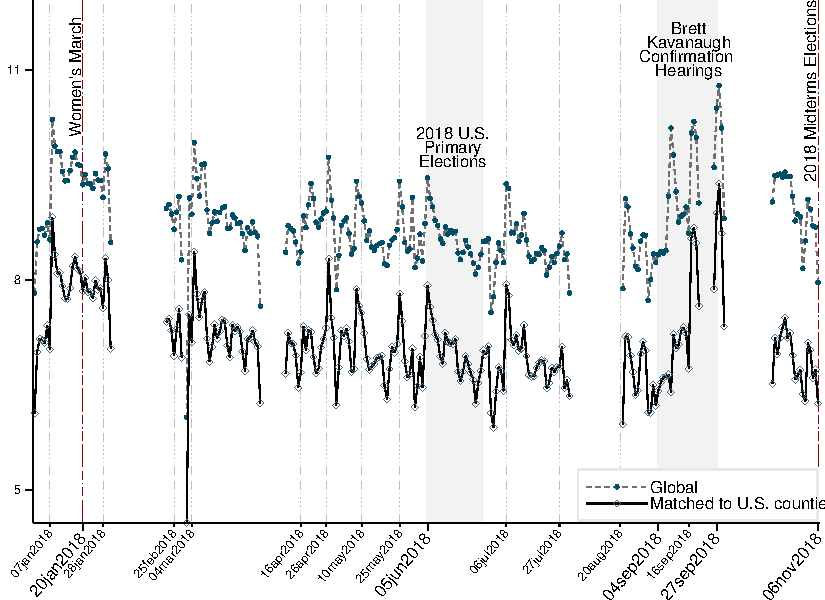
\includegraphics[width=1\textwidth]{figures/tweets-ts.pdf}
	\vspace{-1em}
	\caption{
		Timeline of MeToo Tweets in 2018.\\
		\emph{Note:} \textit{January 7} Golden Globe awards; \textit{January 20} a million people took part in the second annual Women's March on the anniversary of President Donald Trump's oath of office, voicing disapproval of his administration and encouraging people to vote; \textit{January 28} Actor Jeremy Piven accused of sexual assault by three more women; \textit{February 25} Monica Lewinsky writes an essay about her experience with Bill Clinton; \textit{March 4} Oscars; \textit{April 16} \textit{The New York Times} and \textit{The New Yorker} won the \emph{Pulitzer Prize} gold medal for public service for their work on the Harvey Weinstein scandal and sexual assault in general; \textit{April 26} Bill Cosby finally found guilty of sexual assault; \textit{May 10} Spotify no longer plays R. Kelly; \textit{May 25} Harvey Weinstein is taken into police custody; \textit{June 5} 17 states have their primary elections; \textit{July 6} Canada PM Justin Trudeau denies need to conduct investigation of sexual misconduct against him; \textit{July 27} a \textit{New Yorker} article reports that CBS will investigate allegations of sexual misconduct by its CEO Leslie Moonves; \textit{August 20} accuser Asia Argento herself accused of sexual misconduct; and \textit{September 16} a \textit{Washington Post} article revealed Christine Blasey Ford was a victim of sexual assualt by then Supreme Court nominee Brett Kavanaugh.
		See \url{https://web.archive.org/web/20240120220020/https://www.chicagotribune.com/lifestyles/ct-me-too-timeline-20171208-htmlstory.html} for a curation of MeToo events.
	}
	\label{fig:tweets-ts}
\end{figure}

One concern is that the tweets may capture automated bot content \citep{Bessi_Ferrara_2016}.
To filter out such content, I use Botometer X, a bot detection tool that analyzes features such as posting patterns, network characteristics, and account metadata using machine learning \citep{botometer101}.
It returns a probability score between 0 and 1 for bot-like behavior.
I query Botometer X for all 130,402 unique geocoded accounts and drop those with bot scores above 0.5, a threshold that balances precision and recall in bot detection \citep{Bessi_Ferrara_2016, botometer101}, constituting approximately 6.3\% of the queried accounts (\cref{fig:botometer_score_distribution}).
This pipeline yields 324,641 geocoded MeToo tweets.

\cref{fig:tweets-ts} shows the timeline of the geocoded tweets (solid lines), as well as those not matched to US counties (dashed lines).
Although the tweets cannot all be geolocated to US counties (some because they are unambiguously non-US), \cref{fig:tweets-ts} suggests that there is no systematic difference between tweets that can and cannot be matched to US counties.

\subsection{Measuring Local Movement Strength}
\label{sec:local-measure}
To measure the local strength of the MeToo movement using the geocoded \#metoo tweets, I use the county-level population (\cref{sec:ACS}) to normalize tweet activity to get the tweet density measure (tweets per capita).
This normalization isolates variation in local movement traction from variation in county population size, as raw tweet counts mechanically correlate with total county population, and therefore unobserved subpopulation demographics that are more likely to use social media.
As the primary measure of local movement strength, I log the tweet density measure, which addresses skew in the measure, reducing the influence of extreme values on the right tail for a more normally distributed measure suitable for linear regression.%
\footnote{\cref{sm:density-intensity} presents robustness checks using log tweet intensity (without population normalization), with estimates yielding substantively similar conclusions.}

%===============================================================================
\subsection{Election Returns}
The county-level returns of the 2018 House of Representatives election come from the individual states' Secretary of State.
I supplement data on these 40 states with four more states (Arkansas, Michigan, Nevada, and New Mexico) from the \emph{MIT Election Data and Science Lab} (MEDSL).%
\footnote{\url{https://github.com/MEDSL/2018-elections-unoffical}.} 
\footnote{At the time of collection, Alaska's Secretary of State (SOS) page on election results cannot be found, Connecticut, Kansas, Mississippi, and Missouri SOS pages lack voting results at the county or precinct level, and Minnesota has yet to publish their election results.}
I collect 2016 county-level presidential election returns from MEDSL \citep{mitCountyPres}.
For the falsification analyses, I collect the 2016 House election returns as a placebo outcome measure \citep{mitCountyHouse2016}.
To compare changes in turnout from the 2014 midterm elections, I procure the county-level 2014 House election data from David Leip's Atlas of U.S. Presidential Elections \citep{dlusa}.
I merge all datasets using the FIPS (Federal Information Processing Standard) county code, a standardized 5-digit geographic identifier.

%===============================================================================
\subsection{Candidate Characteristics}
For all 1,022 candidates in the 2018 House election, I hand-label their gender and incumbency and systemically infer their ethnicity using \emph{NamePrism}, a supervised algorithm that predicts ethnicity using first and last names and homophily in communication patterns \citep{NamePrism}.%
\footnote{The NamePrism is a supervised classifier developed using 74 million names from an email company. Their Naive Bayes classifier infers nationality/ethnicity using both first and last names (to mitigate migration and marriage), with the likelihood estimated using the homophily principle in communication patterns---people of the same type communicate more frequently and recently.}
From this, each candidate has an indicator for their (predicted) ethnicity (White, Black, Hispanic, or Other).
I use these indicators to adjust for documented identity-based voting behaviors by ethnicity and gender \citep{Abrajano2005, Flanagan2018, HOLLI2010, Matsubayashi2011, Stephens-Davidowitz2014}, as well as to test mechanisms by gender in vote shares and candidacy.
For the falsification analyses, I use the same procedure to code candidates in the 2016 House election.

%===============================================================================
\subsection{County-Level Demographics}
\label{sec:ACS}
County demographics come from the ACS (American Community Survey) 5--year estimates for 2015--2019 \citep{ipums_nhgis}.
These include population and voting population sizes, demographic composition by ethnicity (Black, Hispanic, Other, White), gender, age groups (29 and under, 30 to 64, 65 and over), foreign-born, education levels (college degree and above), income (median household income), employment, and the rural population (\cref{sm:data}).
County-level population is used to normalize the geolocated MeToo tweets for the county-level measures of MeToo tweet density.
I also collect ACS 5--year estimates for 2012--2016 for demographic changes when examining changes in turnout.

%===============================================================================
\subsection{VOTER Survey}
\label{sec:VOTER-data}
To link to and validate the geolocated MeToo tweets, I use the \emph{VOTER} (Views of the Electorate Research) survey \citep{voter}, which tracks about 8,000 individuals from 2012--18 (though some individuals drop out of the study from 2016--18).
VOTER contains detailed measures of political attitudes, including attitudes toward sexism and sexual harassment, approval of political parties' handling of harassment, and self-reported voting behavior in presidential and congressional elections.
I link VOTER respondents to county-level MeToo tweet measures using reported ZIP codes, crosswalked to counties using county FIPS codes from the US Cities Database.
Out of 2,649 counties in the sample, 1,352 counties successfully matched to VOTER microdata, yielding over 6,644 individuals linked to geocoded tweet density measures.
For respondents tracked across waves, I compute changes in attitudes and voting behavior from 2016 to 2018.
The objective is to validate the geolocated MeToo tweets to the extent that they predict the geographical distribution of individual-level pro-women and anti-Republican sentiments, and predict individual-reported voting patterns in the 2016 and 2018 elections.

%===============================================================================
\subsection{Dataset Statistics}
The final sample includes 44 states, 388 congressional districts, and 1,022 House candidates, with 767 as major party candidates.
This gives 8,631 candidate-county observations across 2,650 counties with geocoded and filtered 324 thousand \#metoo tweets.
The distribution of \#metoo tweets across counties is skewed, with an average of 110 per county (median 3, SD 1,063).
The population-normalized measure is 6.8 per 10,000 people (median 1.0, SD 89.4).
At the district level in 2018, 42\% have Republican male incumbents, 27\% Democratic male incumbents, 4\% Republican women incumbents, 12\% Democratic women incumbents, with the last 15\% being open contests.
In total, Democratic women challenged in 30\% of districts while Republican women challenged in 9\%.

%-------------------------------------------------------------------------------
%-------------------------------------------------------------------------------
\section{MeToo Movement and \#metoo Tweets}
\label{sec:background}
%-------------------------------------------------------------------------------
%-------------------------------------------------------------------------------
%===============================================================================
\subsection{MeToo as a Grassroots Social Movement}
\label{sec:mt-background}
Social movements and elections have traditionally been studied as distinct domains of democracy and representation \citep{McAdam_Tarrow_2010}.
However, social and grassroots movements---especially those amplified through social media---can shape political discourses and electoral outcomes \citep{Amenta2010, Gibson2019, elitestweet, thomsen2020, womenmarch, kim2022, leon2022, cs, weiss2022, sobolev2020, Acemoglu2018, Eisele2022}.

The decentralized nature of social media bypasses traditional media gatekeeping \citep[e.g.,][]{AEP2015, Boas2011, Enikolopov2011}, empowering political actors to engage with the movements at scale \citep{elitestweet, cs, womenmarch, dittmar2020}.
This dynamic was evident with the MeToo movement, where the movement's momentum on Twitter precipitated into politically charged public protests by the time of the 2018 elections \citep{Eisele2022, dittmar2020, Gibson2019, womenmarch, thomsen2020, DeMora2023}.

%===============================================================================
\subsection{A Brief Timeline}
\label{sec:mt-timeline}
The phrase ``Me Too'' originated in 2006 on Myspace, where Tarana Burke used it to support Black and Hispanic women speaking out against sexual misconduct \citep{Eisele2022, Gibson2019}.
More than a decade later, the movement gained momentum when more celebrities shared their experiences on Twitter, turning private trauma into a national conversation \citep{goenaga2021}. 
By 2018, it fueled demand for real change through legislation in Congress that could come from a change in political leadership from voting more women into Congress \citep{genderwatch2018, telegraphMetoo, tippett2018-bi,thomsen2020, nyt2018}. 

\begin{figure}[tbp]
	\centering
	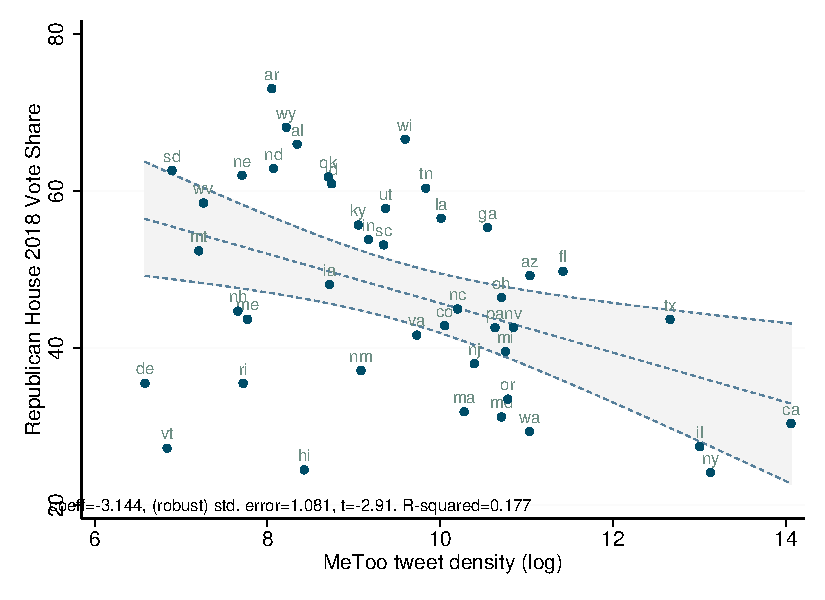
\includegraphics[width=0.65\linewidth]{figures/state-level.pdf} \vspace{-1em} 
	\caption{
		State-Level Republican Vote Share and MeToo Movement.\\
		\emph{Note:} The figure reports the bivariate relationship between the 2018 Republican House vote share and the log MeToo tweet density at the state level from a simple linear regression.
		Please see \cref{sec:data} for the underlying data.
		The gray shaded area is the 95\% confidence interval around the fitted line.
	}
	\label{fig:state-level} 
\end{figure}

The movement took center stage just before the midterm elections, particularly during Brett Kavanaugh's Supreme Court confirmation hearings (\cref{fig:tweets-ts}).
The hearings, combined with existing allegations against President Trump, meant the movement propelled the midterms towards a nationalized referendum on the \R{} administration \citep{Lucas2021, CarsonHitefield2018, Gibson2019, dittmar2020, DeMora2023}.
Spikes in the online movement can also be traced back to high-profile events like the Cosby trial and the second Kavanaugh confirmation hearing (\cref{fig:tweets-ts}).
The MeToo movement, combined with the amplification of social media, is thus proposed to have influenced the 2018 elections \citep{McAdam_Tarrow_2010}.
\cref{fig:state-level}, for example, provides descriptive evidence that states with higher MeToo movement, as measured by the MeToo tweets (\cref{sec:local-measure}), have lower Republican vote shares.

%===============================================================================
\subsection{\#metoo Tweet Samples}
\label{sec:tweet-samples}
\cref{tab:random-sample} enumerates a random sample of 20 tweets from the geocoded MeToo tweet dataset (\cref{sec:local-measure}).
Most exhibit substantive engagement with the movement, including sharing personal survivor testimonies, related news about specific allegations (e.g., Schneiderman, Franco), harassment-related legislation, and critical dialogue of the movement.
One tweet is unclear and possibly a co-opting of the hashtag for gun rights advocacy (``\textit{So any woman who supports the second amendment (myself and MANY OTHERS) deserve to be spoken to this way?}''), one runs counter to the movement as it is used rhetorically in political criticism of Democrats (e.g., ``\textit{@SenFeinstein Dirty Dianne what about this accusation where are the \#MeToo pink nasty hat wearing females?}''), and two are unsubstantial with just a single hashtag or comedic observation (e.g., a bare MeToo hashtag and \textit{``Maybe all this \#metoo stuff is creating an uptick in women's drinking habits''}).
In \cref{sm:random-samples}, I select four key political events and randomly sample 20 tweets from their specific dates: State of the Union (January 31), Women's March (January 21), Christine Blasey Ford's public revelation (September 17), and Kavanaugh confirmation hearings.
From these additional conditional random samples of \#metoo tweets, I find similar rates ($\sim$80\%) of substantive engagement with the movement.

To supplement my manual assessment of these random tweets, I use large language models (LLM) to both corroborate my coding and to scale the evaluation.
First, I use a zero-shot classification using a prompt providing a definition of what tweet content could be genuine reflections of the MeToo discourse (e.g., political discussions around key related events, personal experiences of harassment or assault, protest movements, and general expressions of solidarity and support, see \cref{sec:tweet-content}), and what could be disingenuous usage (e.g., ironic uses or attacks on the Democratic Party and survivors).
This procedure yields a 93\% agreement between the resulting classifications and my manual labels.
Next, to scale this classification beyond the initial 100 tweets, I randomly sample 5000 more tweets, and provide a fixed, randomly drawn set of 10 labeled tweets (from the initial 100) directly in the LLM prompt for examples of \#metoo tweets in a few-shot classification task.
This classification suggests that close to three-quarters of the sample reflects the MeToo discourse (\cref{sm:random-samples}).

\begin{table}[tbp]
	\centering
	\scriptsize
	\setlength{\defaultaddspace}{2pt}
	\setlength\tabcolsep{3 pt}
	\caption{Random Sample of \#metoo Tweets}
	\label{tab:random-sample}
	\begin{adjustbox}{max width=1\textwidth}	
		\begin{tabular}{@{\hspace{0\tabcolsep}}p{1.3cm}rr>{\raggedright\arraybackslash}p{3.2cm}>{\raggedright\arraybackslash}p{15cm}@{\hspace{0\tabcolsep}}}
			\toprule
			Date & Fave & RT & Other hashtags & Tweet content \\
			\midrule
			2018-09-13 & 5 & 1 & \#blacklivesmatter, \#oupsm & The \#MeToo and \#BlackLivesMatter movements both came from a person or people with a desire to change society because of negative experiences. These hashtags found strength in social media to fight oppression. However, \#BlackLivesMatter faced more backlash. \\
			\addlinespace
			2018-01-25 & 4 & 0 & --- & Because I will scream if I hear this misused again, one more reminder: a ``witch hunt'' is, by definition, a panic over a nonexistent or severely overstated threat. It does not apply to real threats. Sexual assault is real and pervasive. Therefore, \#MeToo isn't a witch hunt. \\
			\addlinespace
			2018-02-27 & 0 & 0 & --- & Maybe all this \#metoo stuff is creating an uptick in women's drinking habits... [Twitter URL] \\
			\addlinespace
			2018-01-13 & 2 & 1 & --- & A month or so ago, a friend and I mulled over when exactly the backlash to the then-peaking \#MeToo moral panic would set in. Mid-January, we guessed, and sure enough, here's Andrew Sullivan jumping on the train lest he get left behind. [Twitter URL] \\
			\addlinespace
			2018-05-09 & 0 & 0 & --- & Eric Schneiderman's \#MeToo Hypocricy [YouTube URL] \\
			\addlinespace
			2018-07-16 & 0 & 0 & --- & \#metoo \\
			\addlinespace
			2018-01-12 & 1 & 0 & --- & I would have thought that \#metoo would have showed us that no group has a monopoly on hypocritical disgusting predators. \\
			\addlinespace
			2018-05-25 & 0 & 0 & --- & The man who pinned me down had handcuffs on today. - Rose McGowan on @MegynTODAY \#metoo \\
			\addlinespace
			2018-10-20 & 12 & 10 & --- & Survivors don't owe us. We owe them. \#MeToo [URL] \\
			\addlinespace
			2018-06-03 & 0 & 0 & --- & @CathyYoung63 who are the feminists you are reading who focus mostly on ``bashing men for trivial transgressions.'' I read Ijeoma Oluo, Aminatou Sow, Ruth Bader Ginsburg, Chimamanda Ngozi Adichie, Lindy West, Caitlin Flanagan, and while they spoke out in support of \#metoo \\
			\addlinespace
			2018-06-01 & 24 & 0 & --- & [Persian/Arabic text] \#MeToo \\
			\addlinespace
			2018-04-18 & 1 & 0 & --- & Susan Fowler-Uber \#metoo When I reported the situation, I was told by HR \& upper management that this was sexual harassment \& he was propositioning me, it was this man's 1st offense, \& they wouldn't feel comfortable giving him anything other than a warning. He ``was a high performer.'' \\
			\addlinespace
			2018-01-12 & 0 & 0 & --- & \#MeToo James Franco Accused of Sexual Misconduct By Five Women [URL] \\
			\addlinespace
			2018-03-23 & 2 & 1 & \#sexualharassment, \#france, \#womensrights & Is a wolf whistle worth \$100? France considers on-the-spot fines for street harassment in new legislation [Reuters URL] \\
			\addlinespace
			2018-01-10 & 8 & 7 & \#pasmoi & France, Where \#MeToo Becomes \#PasMoi. Some notable French women are decrying a ``puritanical'' wave of reckoning over sexual misconduct. [Atlantic URL] \\
			\addlinespace
			2018-05-09 & 1 & 0 & --- & After shocking allegations of sexual abuse, champion of the \#MeToo movement, NY AG Eric Schneiderman resigns from office. [URL] \\
			\addlinespace
			2018-09-12 & 0 & 0 & \#crazy, \#maga, \#stopthehate & So any woman who supports the second amendment (myself and MANY OTHERS) deserve to be spoken to this way? \#MeToo \#Crazy \#maga \#Stopthehate \\
			\addlinespace
			2018-09-19 & 0 & 0 & \#biased, \#liberalismisamentaldisease & @SenFeinstein Dirty Dianne what about this accusation where are the \#MeToo pink nasty hat wearing females? \#biased \#LiberalismIsAMentalDisease \\
			\addlinespace
			2018-06-29 & 0 & 0 & --- & Russell Simmons, an `Extra' Host and NBC News: A Sexual Assault Accuser's Story of Pain and Frustration [Hollywood Reporter URL] \#metoo \\
			\addlinespace
			2018-05-01 & 2 & 0 & \#timesup, \#resist, \#blm, \#daca, \#marchforourlives & May Day \#MayDay Why I Still \#Resist \#POTUS \#LiarLiar \#GOP \#Traitor \#DACA \#LGBTQ \#MeToo \#TimesUp \#BlackLivesMatter \#MarchForOurLives [...] \\
			\bottomrule
		\end{tabular}
	\end{adjustbox}
	\caption*{
		\scriptsize
		\textit{Note:} 
		Random sample is seeded for replicability.
		Fave = number of favorites; RT = number of retweets.
		Please see \cref{sm:random-samples} for more random samples.
	}
\end{table}

\begin{figure}[tbp]
	\centering
	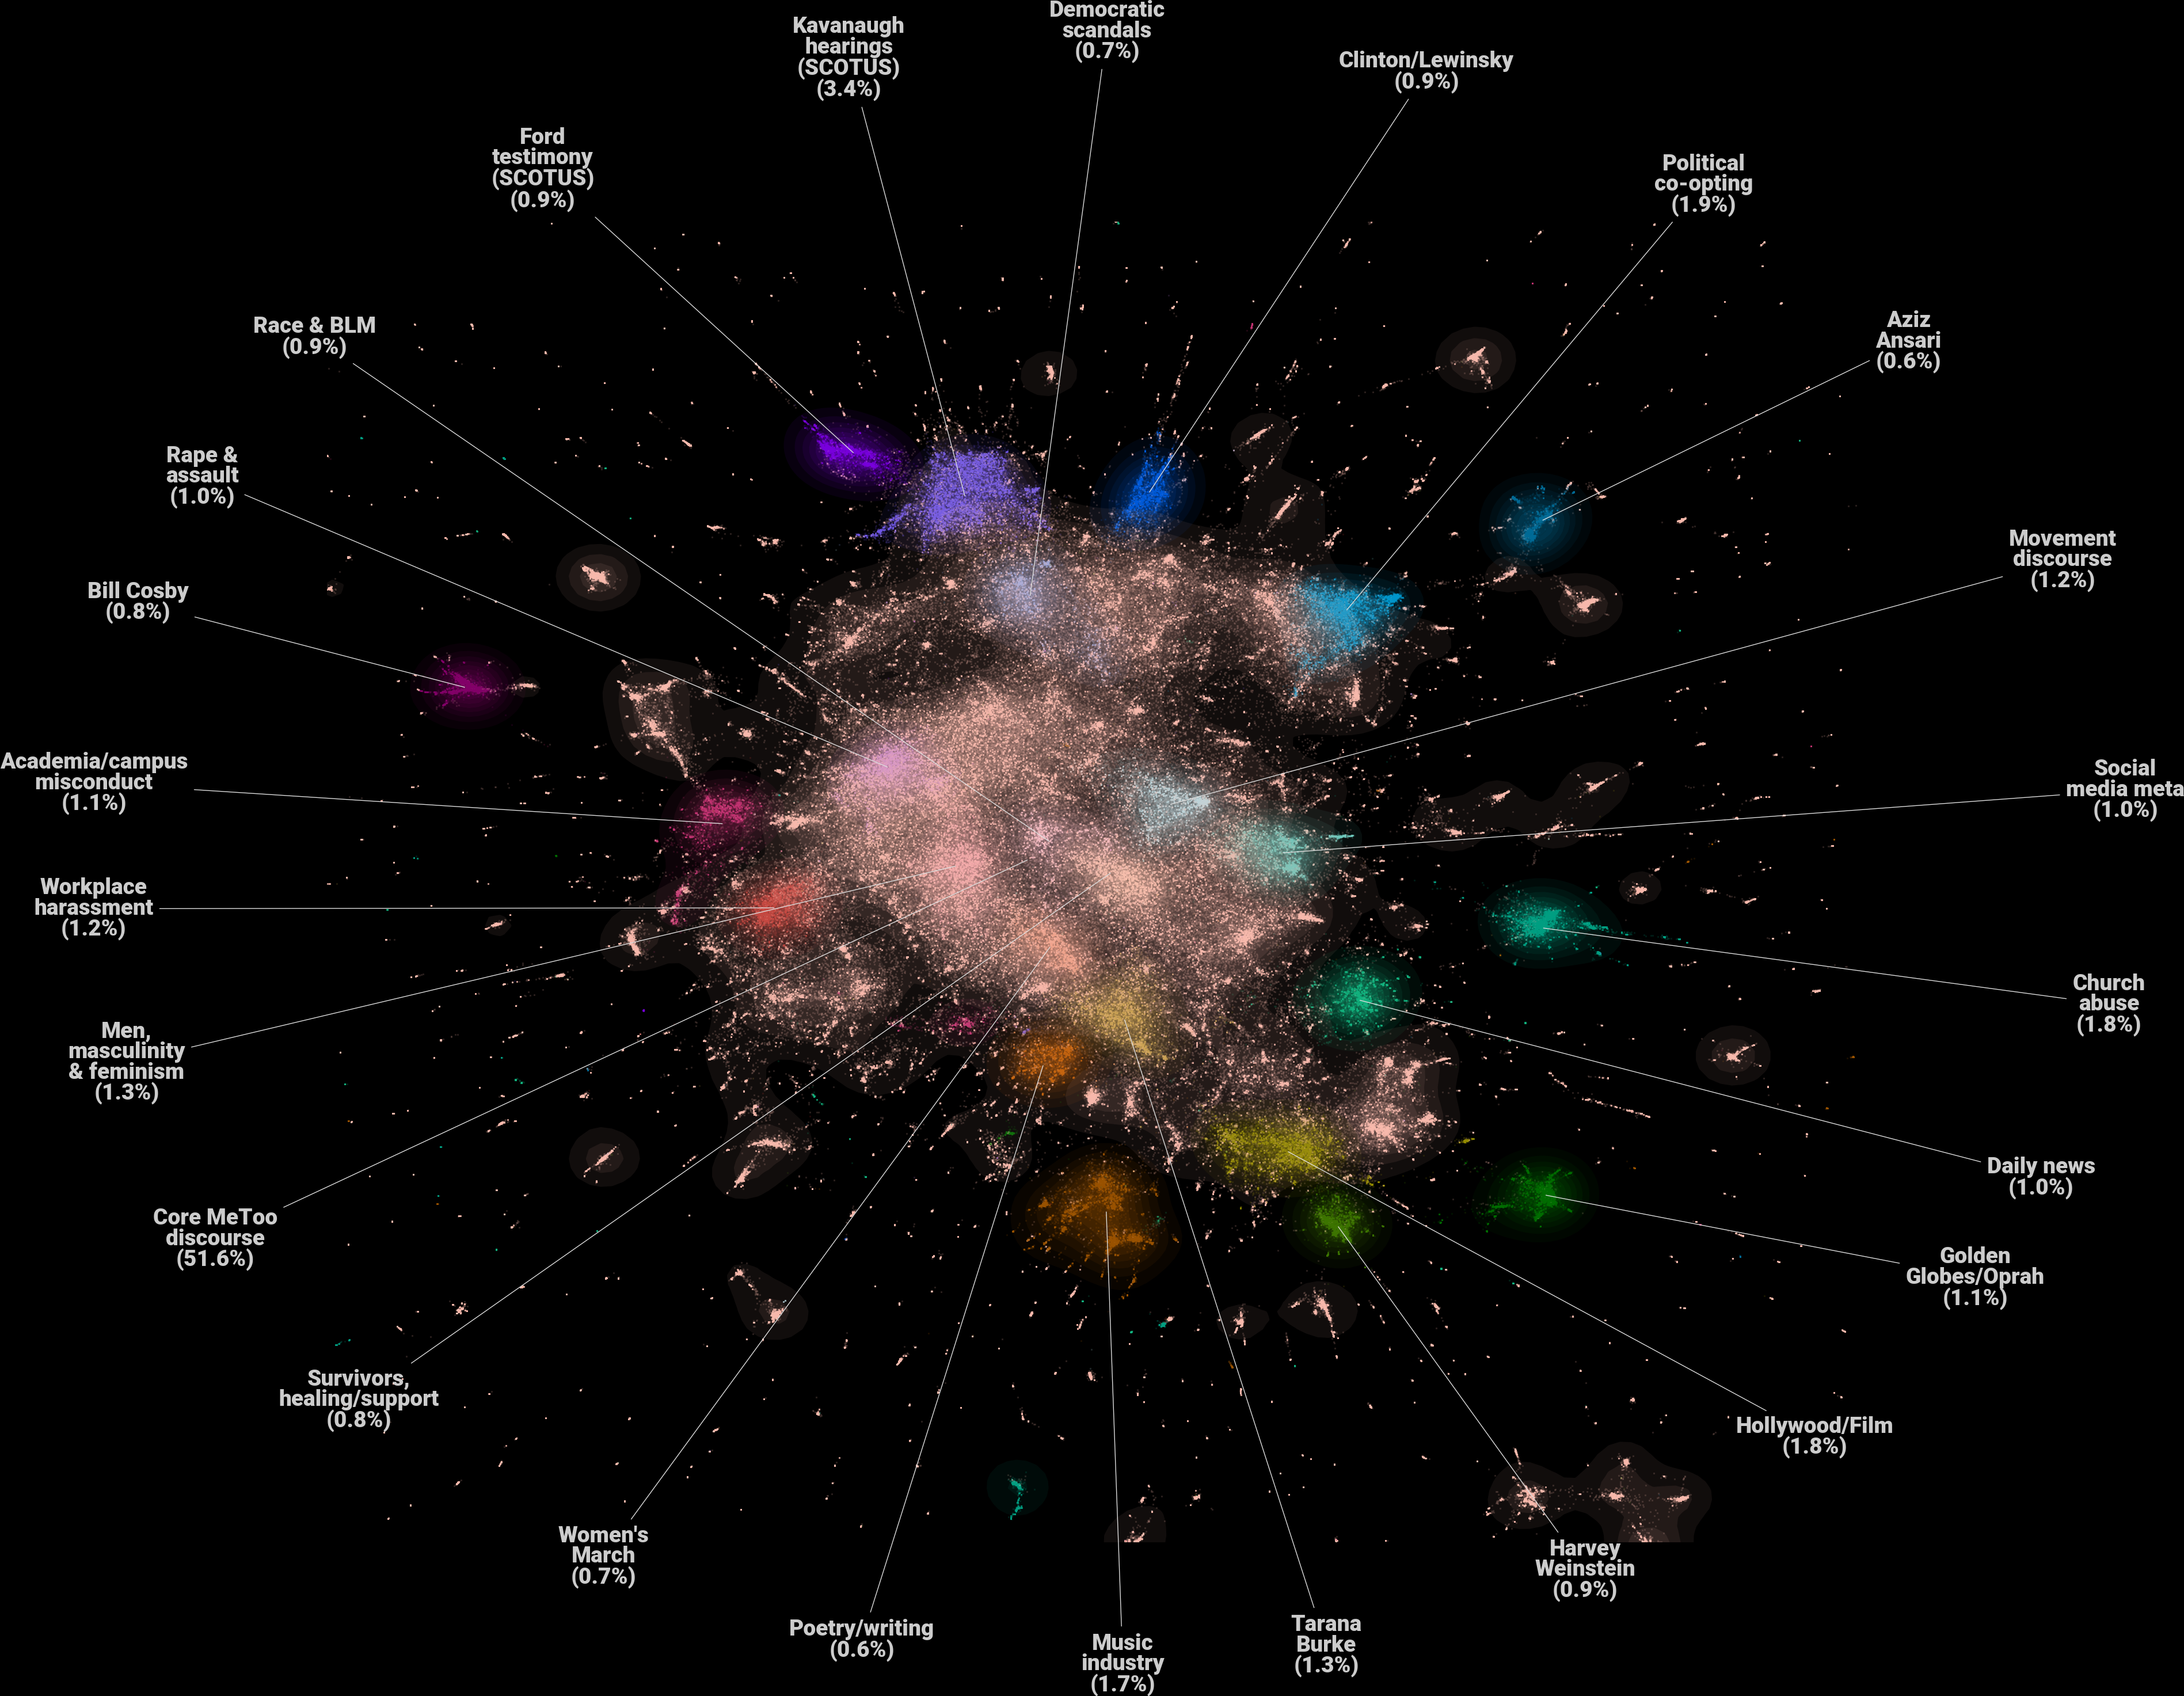
\includegraphics[width=\linewidth]{figures/topic_2Dmap_darkmode.png}
	\caption{
		Two-Dimensional Visualization of \#metoo Tweet Topics.\\
		Notes: The Tweet text us encoded into 768-dimensional embeddings, then projected to 2D space using UMAP dimensionality reduction that preserves the relationship between tweets for visualization.
		Topics are identified with BERTopic.
		Each point is a tweet, and clusters of colored points represent topics.
		These 25 topics collectively account for over 87\% of the tweet sample.		
		See \cref{fig:top_topics_tabulation} for the corresponding top words of each topic.
	}
	\label{fig:topic_2Dmap}
\end{figure}

\begin{figure}[tbp]
	\centering
	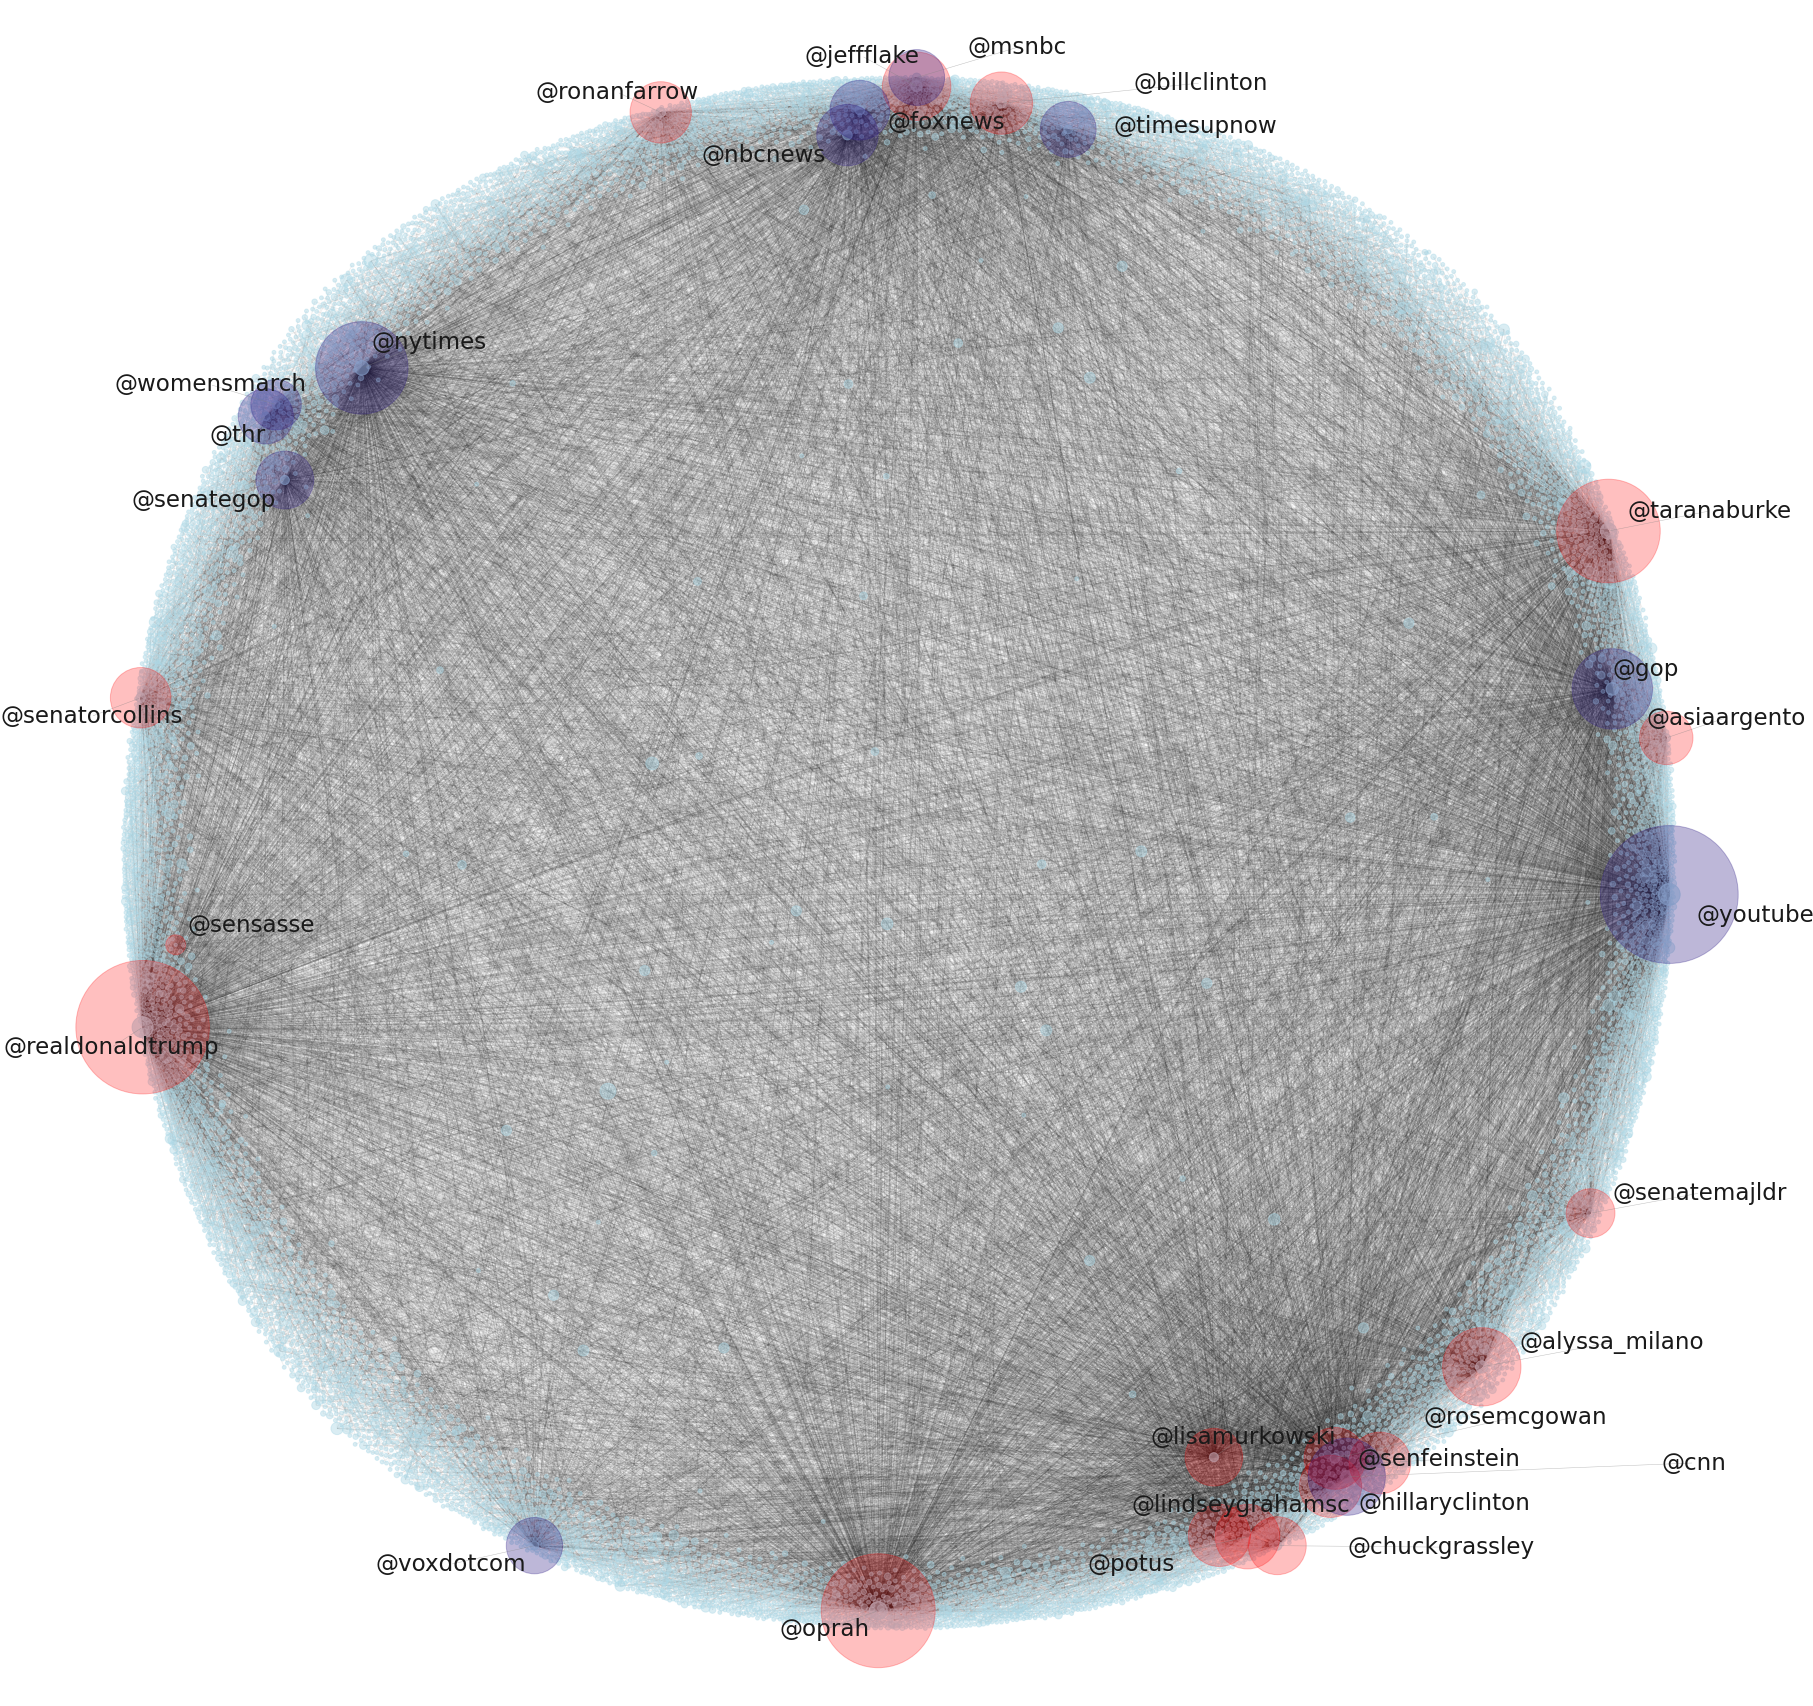
\includegraphics[width=\linewidth]{figures/network_mentions.png}
	\caption{
		Network of 30 most-mentioned accounts.\\
		Notes: Light blue nodes represent individual Twitter users.
		Red nodes represent individuals; purple nodes represent organizations and media outlets.
		Node size reflects mention frequency for red/purple nodes and user activity for blue nodes.
	}
	\label{fig:network_mentions}
\end{figure}

%===============================================================================
\subsection{Tweet Content}
\label{sec:tweet-content}
To provide evidence that the \#metoo tweet sample's engagement patterns and semantic content captures the documented MeToo discourse in 2018 as discussed in \crefrange{sec:mt-background}{sec:mt-timeline}, I clean and deduplicate the raw text (e.g., ``i support the \#metoo metoo movement \#metoo movement!!!'' $\longrightarrow$ ``i support the \#metoo movement!'') before analyzing them (please see \cref{sm:text} for full details).

To uncover clusters of semantically-aware tweets revolving around themes in the MeToo discourse, I apply a transformer-based topic modeling approach using BERTopic  \citep{bertopic}.
The topic modeling confirms that the majority of tweets relate to salient and relevant issues (\cref{fig:topic_2Dmap}), with the core discourse topic (51.6\%) containing keywords such as women, movement, men, and timesup.
Substantive themes emerge around specific high-profile cases aligned to real-world events in 2018, such as the Kavanaugh and Ford hearings around the Supreme Court confirmation (see also \cref{fig:tweets-ts}).
Other top identified topics include the revived conversation around Clinton--Lewinsky, stories around sexual assault, survivors, and support, Hollywood figures including Weinstein, and the conversation around workplace harassment and HR policies.

Hashtags that co-occur with \#metoo relate to electoral mobilization tags (voteblue2018, bluewave, timesup, p2 [Progressives 2.0], marchforourlives, votethemout2018; \cref{fig:network_hashtags}), and concentrated attention on the Kavanaugh hearings (\#kavanaugh), with the highest engagement on \#kavanaughhearings (10.2 retweets, 32.2 favorites; \cref{fig:top_hashtags_tabulation}).

Anti-Trump tags are prominent (e.g., impeachtrump, arresttrumpcrimefamily, votethemout2018, bonespursunfit, 25trump, dumptrump), who was himself a top mention in the tweet network (``@realdonaldtrump'', \cref{fig:network_mentions}), consistent with the movement positioned as a referendum on the Trump administration.
Other frequently mentioned accounts center on figures involved in 2018 political controversies: Kavanaugh and Blasey Ford, and the senators who voted on the nomination (Collins, Flake, Murkowski, Feinstein, Graham).
Tarana Burke, the founder of MeToo (\cref{sec:mt-timeline}), is a frequent mention, as are minor celebrities in the origin of the movement.
Top web domains from the URL analysis reveal the presence of major news outlets (e.g., nytimes.com, theguardian.com, washingtonpost.com, wapo.st, huffingtonpost.com), many of which are shared with high retweets and favorites (\cref{fig:top_domains_tabulation}).
All these patterns are confirmed using Named Entity Recognition (\cref{tab:ner_results}).
Many of these political figures and entities are also in the network of top mentions (\cref{fig:network_mentions}).

%===============================================================================
\subsection{Individual-Level Attitudes}
\label{sec:VOTER-validation}
To further validate that the geolocated MeToo tweets reflect genuine grassroots discourse, I combine them with microdata from the VOTER survey (\cref{sec:VOTER-data}).
If tweets reflect authentic movement mobilization rather than astroturfing,%
\footnote{Astroturfing is the practice of coordinated but inauthentic political activity masquerading as true grassroots activity.}
individuals residing in counties with strong movement traction should exhibit attitudes aligning with those of the movement.

Overall, I find that the tweets capture individual-level pro-feminist (anti-sexism) and anti-Republican attitudes.
Specifically, individuals living in areas with more MeToo tweets are less likely to produce responses consistent with sexism based on items on gender roles and sexual harassment.
They are also less likely to approve of the Republican Party's handling of harassment and assault in politics, with this pattern absent for the Democratic Party.
In terms of self-reported voting history, these individuals are also less likely to vote Republican in 2016 and 2018, and more likely to switch from Republican to Democrat.
These individual-level patterns hold after adjusting for demographics, political interest, and voting history, and are consistent with the MeToo tweets capturing issue salience \citep[e.g.,][]{sobolev2020} rather than coordinated astroturfing  (\cref{sm:VOTER}).

%-------------------------------------------------------------------------------
%-------------------------------------------------------------------------------
\section{Candidate Vote Shares}
\label{sec:voteshare}
%-------------------------------------------------------------------------------
%-------------------------------------------------------------------------------
The 2018 midterms elections were widely characterized as a ``\#MeToo election'', with gender issues shaping the outcome to the advantage of the Democratic party \citep{genderwatch2018, telegraphMetoo, tippett2018-bi,thomsen2020, cs}.
On the surface, this appeared to be true given that the state-level \R{} vote shares decrease with the strength of the movement (\cref{fig:state-level}).
This aggregate pattern, however, could reflect multiple mechanisms.

First, the movement may have garnered greater support for women candidates, particularly Democratic ones, given the movement's alignment with Democratic party positions on gender issues, including those relating to workplace harassment and related legislation (\cref{sec:background}, see also \cref{sm:legal}).%
\footnote{\label{fn:legal}\cref{sm:legal} summarizes some legal implications of the MeToo movement, including bills related to sexual harassment, such as the limits of non-disclosure agreements and recall elections.}
If the movement persuaded voters at the margin on such issues, Democratic women should receive higher vote shares in areas with stronger local movement activity.

Second, this association may be intensified in Republican areas, given the movement's opposition towards the Trump administration (\cref{sec:background}).
In strongly Republican areas, the discourse's highlighting of the Trump administration and Republican responses to misconduct allegations, including the highly salient and controversial Kavanaugh hearings (\cref{sec:background}), could have intensified tensions between partisan loyalties and the national conversation around gender representation and accountability.
Party loyalty was lower among Republican voters in the 2016 elections \citep{KeeterIgielnik2020}, and the movement may have appealed to their demand for gender representativeness over typical partisan alignment \citep{Lucas2021, CarsonHitefield2018, Gibson2019, dittmar2020, DeMora2023, brookings2019turnout2}.
If the local MeToo discourse indeed led voters to defect from their typical \R{} partisan alignment, Democratic candidates---especially women---should receive higher vote shares in Republican counties where the movement had greater traction.
I test for such heterogeneity by testing whether the relationship between the movement and vote shares varies with Trump's 2016 presidential vote share.

Alternatively, the state-level correlation between Republican vote shares and the level of the MeToo movement (\cref{fig:state-level}) could reflect pre-existing demographic patterns unrelated to the movement itself.
To test this, I also examine whether associations are detectable when linking the 2018 MeToo tweet measures with the 2016 House election returns.
If similar patterns exist, even after adjusting for local demographics, then it suggests that the correlation reflects broader electoral shifts that predate the movement.

%===============================================================================
\subsection{Estimation}
\label{sec:voteshare-estimation}

To test whether candidate-level vote shares depend on the MeToo movement, I compare county-level returns of candidates based on their party--gender and the local MeToo tweet density:
\begin{multline}
\label{eq:voteshare}
\nu_{ic} = 
\beta^{RW} RW_i \tau_c + 
\beta^{DW} DW_i \tau_c + 
\beta^{RM} RM_i \tau_c + 
\beta^{DM} DM_i \tau_c\\ 
+ \text{Candidate}_i + 
\bm{\Delta}_1  \bm{\nu}^{\text{Rep., House}}_{c, 2016}  + 
\bm{\Delta}_2  \bm{\nu}^{\text{Rep., Pres.}}_{c, 2012-2016} + 
\bm{\Gamma} \bm{X}_{ic} + 
\varepsilon_{ic},
\end{multline}
where $\nu_{ic}$ is the vote share of the 2018 House candidate $i$ in county $c$.
$\tau_c$ is the county-level log of tweet density (county MeToo tweets divided by population).
$RW_i$, $DW_i$, $RM_i$, and $DM_i$ indicate Republican women, Democratic women, Republican men, and Democratic men, respectively.
Each indicator equals 1 if candidate $i$ belongs to that party-gender category, and 0 otherwise.
$\hat{\beta}^{DW} > 0$ would imply an advantage for Democratic women in counties with stronger MeToo activity.

$\bm{X}_{ic}$ includes county demographics interacted with candidate party, and candidate gender/ethnicity interacted with corresponding county composition, allowing for demographic voting patterns and identity-based heuristics \citep{EdlundPande2002, Abrajano2005, Herron2005, HOLLI2010, Oswald2010, Stephens-Davidowitz2014, Flanagan2018}.
$\bm{\nu}^{\text{Rep., House}}_{c, 2016}$ and $\bm{\nu}^{\text{Rep., Pres.}}_{c, 2012-2016}$ are party-interacted 2016 House and 2012-2016 presidential vote shares, adjusting for existing political support.
Candidate fixed effects control for a constant level of political support across counties.
The full-sample regressions include third-party candidates.
The standard errors are clustered by candidate since their vote shares are correlated across counties.%
\footnote{A well-known pattern during the midterms is a depression of the vote share for candidates from the same party as the sitting president.
	Candidate fixed effects absorb party-specific baseline support, including any aggregate midterm penalty for the president's party.}

\subsubsection{Heterogeneity by 2016 Republican Presidential Vote Share}

I additionally examine if local support for Trump in the 2016 presidential elections moderates the relationship between the movement and candidate vote shares (\cref{sec:background}).
To formally test this, I add an additional interaction to \cref{eq:voteshare} for the county-level Republican vote share from the 2016 presidential election:
\begin{equation}
\begin{split}
\label{eq:repPres}
\nu_{icd} = \alpha &+ \beta^{RW} (RW_i) \tau_c + \gamma^{RW}(RW_i)\tau_c \nu^{\text{Rep., Pres.}}_{c,\ 2016}\\
&+ \beta^{DW} (DW_i) \tau_c + \gamma^{DW}(DW_i)\tau_c \nu^{\text{Rep., Pres.}}_{c,\ 2016}\\
&+ \beta^{RM} (RM_i) \tau_c + \gamma^{RM}(RM_i)\tau_c \nu^{\text{Rep., Pres.}}_{c,\ 2016}\\
&+ \beta^{DM} (DM_i) \tau_c + \gamma^{DM}(DM_i)\tau_c \nu^{\text{Rep., Pres.}}_{c,\ 2016}\\
&+ \text{Candidate}_i + \bm{\Delta}_1 \bm{\nu}^{\text{Rep., House}}_{c, 2016} + \bm{\Delta}_2 \bm{\nu}^{\text{Rep., Pres.}}_{c, 2012-2016}\\
&+ \bm{\Gamma} \bm{X}_{ic} + \varepsilon_{icd},
\end{split}
\end{equation}
%%%%%%%%%%%%%%%%%%%%%%%%%%%%%%%%%%%%%%%%% EQUATION %%%%%%%%%%%%%%%%%%%%%%%%%%%%%%%%%%%%%%%%%%%%%%%%%
where the primary coefficients of interest are the $\gamma^{(.)}$ terms, capturing heterogeneity by 2016 Trump support.
For instance, $\hat{\gamma}^{DW}>0$ implies Democratic women perform better where MeToo activity is higher, and Trump support was stronger.
The 2016 presidential vote share is centered at 50\%, so $\hat{\beta}$ terms reflect effects at 50-50 partisan splits.

%===============================================================================
\subsection{Results}
\label{sec:voteshare-results}

\begin{table}[tbp]
	\centering \footnotesize \setlength\tabcolsep{4 pt} \setlength{\defaultaddspace}{-1pt}
	\def\sym#1{\ifmmode^{#1}\else\(^{#1}\)\fi}
	\caption{MeToo Movement and Candidate Vote Share}
	\label{tab:voteshare}
	\begin{adjustbox}{max width=1\textwidth}
		\begin{tabular}{@{\hspace{0\tabcolsep}}l*{4}{D{.}{.}{-1}}@{\hspace{0\tabcolsep}}}
			\toprule\toprule
			&&&\multicolumn{2}{c}{Heterogeneous effect, by pres.}\\
			&&&\multicolumn{2}{c}{\R{} vote share in 2016}\\
			\cmidrule(l){4-5}
			&\multicolumn{3}{c}{All-party share}&\multicolumn{1}{c}{Two-party share}\\
			\cmidrule(lr){2-4}\cmidrule(l){5-5}
			&\multicolumn{1}{c}{(1)}&\multicolumn{1}{c}{(2)}&\multicolumn{1}{c}{(3)}&\multicolumn{1}{c}{(4)}\\
			\midrule
			Log tweet density $ \times $ (Rep. woman)&   -4.458\sym{***}&   -0.208         &   -0.404         &   -0.066         \\
          &  (1.674)         &  (1.162)         &  (1.488)         &  (1.363)         \\
Log tweet density $ \times $ (Dem. woman)&    0.707         &   -0.241         &   -0.920         &   -1.028         \\
          &  (0.575)         &  (0.453)         &  (0.607)         &  (0.709)         \\
Log tweet density $ \times $ (Rep. man)&   -3.235\sym{***}&   -0.118         &    0.062         &    0.183         \\
          &  (0.547)         &  (0.351)         &  (0.472)         &  (0.524)         \\
Log tweet density $ \times $ (Dem. man)&   -0.133         &   -0.737\sym{**} &   -1.380\sym{**} &   -1.405\sym{**} \\
          &  (0.412)         &  (0.367)         &  (0.587)         &  (0.678)         \\
Log tweet density $ \times $ (Pres. 2016 Rep. vote share) $ \times $ (Rep. woman)&                  &                  &   -0.049         &   -0.055         \\
          &                  &                  &  (0.044)         &  (0.038)         \\
Log tweet density $ \times $ (Pres. 2016 Rep. vote share) $ \times $ (Dem. woman)&                  &                  &    0.067\sym{**} &    0.073\sym{**} \\
          &                  &                  &  (0.031)         &  (0.031)         \\
Log tweet density $ \times $ (Pres. 2016 Rep. vote share) $ \times $ (Rep. man)  &                  &                  &   -0.011         &   -0.014         \\
          &                  &                  &  (0.017)         &  (0.018)         \\
Log tweet density $ \times $ (Pres. 2016 Rep. vote share) $ \times $ (Dem. man)  &                  &                  &    0.054\sym{**} &    0.049\sym{**} \\
          &                  &                  &  (0.021)         &  (0.022)         \\
\emph{Control variables}&                  &                  &                  &                  \\
\hspace{1em}Candidate fixed effects&\multicolumn{1}{c}{$ X $}         &\multicolumn{1}{c}{$ X $}         &\multicolumn{1}{c}{$ X $}         &\multicolumn{1}{c}{$ X $}         \\
\hspace{1em}2016 House \& 2012--16 Pres. election&                  &\multicolumn{1}{c}{$ X $}         &\multicolumn{1}{c}{$ X $}         &\multicolumn{1}{c}{$ X $}         \\
\hspace{1em}County census demographics&                  &\multicolumn{1}{c}{$ X $}         &\multicolumn{1}{c}{$ X $}         &\multicolumn{1}{c}{$ X $}         \\
\hspace{1em}Racial \& gender voting&                  &\multicolumn{1}{c}{$ X $}         &\multicolumn{1}{c}{$ X $}         &\multicolumn{1}{c}{$ X $}         \\
$ F $-test: House \& 2012--16 Pres. election = 0&                  &\multicolumn{1}{c}{$ F = 71.09^{***} $}         &\multicolumn{1}{c}{$ F = 12.31^{***} $}         &\multicolumn{1}{c}{$ F = 4^{**} $}         \\
$ F $-test: Census controls = 0&                  &\multicolumn{1}{c}{$ F = 6.87^{***} $}         &\multicolumn{1}{c}{$ F = 6.78^{***} $}         &\multicolumn{1}{c}{$ F = 8.7^{***} $}         \\
$ F $-test: Racial \& gender voting = 0&                  &\multicolumn{1}{c}{$ F = 3.47^{***} $}         &\multicolumn{1}{c}{$ F = 3.56^{***} $}         &\multicolumn{1}{c}{$ F = 6.71^{***} $}         \\
Main-party candidates only&                  &                  &                  &\multicolumn{1}{c}{$ X $}         \\
$ R^2 $   &    0.794         &    0.876         &    0.877         &    0.798         \\
$ N $     &\multicolumn{1}{c}{$ 8631 $}         &\multicolumn{1}{c}{$ 8455 $}         &\multicolumn{1}{c}{$ 8455 $}         &\multicolumn{1}{c}{$ 6223 $}         \\
			\bottomrule
		\end{tabular}
	\end{adjustbox}
	\caption*{
		\footnotesize
		\emph{Notes:}
		The dependent variable is the candidate's vote share at the district-county level.
		Estimates from modeling candidate vote share as dependent on the politician's party-gender and the MeToo movement measured using the MeToo tweet density (normalized by county population) in 2018 at the county level (\cref{sec:voteshare-estimation}).
		The Republican presidential vote share is centered at 50\%.
		Columns (3)--(4) additionally condition the effect of party-gender and the MeToo movement on existing Republican support.
		Coefficients for third-party candidates not reported to conserve space.
		Significance levels: $^*$ 0.1 $^{**}$ 0.05 $^{***}$ 0.01.
	}
\end{table}

\cref{tab:voteshare} reports the results for candidate-level vote share (\cref{sec:voteshare-estimation}).

In Column (1), with only candidate fixed effects, Republican candidates (both men and women) received lower vote shares in counties with higher MeToo activity.
Column (2) adds past electoral controls, county demographics, and ethnic- and gender-based voting controls.
With these controls, the Republican estimates attenuate to null, while Democratic men show a marginally significant negative relationship.

The average effects in Columns (1)--(2) (\cref{tab:voteshare}), however, may mask heterogeneous effects.
Columns (3)--(4) report estimates from \cref{eq:repPres}, revealing significant heterogeneity.
Column (4)'s two-party interaction coefficients for Democratic women ($\hat{\gamma}^{DW} = 0.073$, $p < .05$) and Democratic men ($\hat{\gamma}^{DM} = 0.049$, $p < .05$) indicate that both performed relatively better in Republican-leaning counties with high MeToo activity.
No such heterogeneity exists for Republican candidates.
For Democratic women, a standard deviation increase in MeToo activity is associated with a 1.61 percentage point ($0.073 \times 20 \times 1.103$) larger effect in counties where Trump won 70\% versus 50\%.%
\footnote{The point estimates suggest Democratic women experience absolute positive effects in counties where the 2016 Republican presidential vote share exceeded approximately 64\%, while Democratic men would break even only where Trump won approximately 79\% of the vote.}
% Democratic women: -1.028 + 0.073 × (breakeven - 50) > 0
%                    0.073 × (breakeven - 50) > 1.028
%                    breakeven - 50 = 1.028 / 0.073 > 14.08
%                    breakeven > 64.08%
% Democratic men:   -1.405 + 0.049 × (breakeven - 50) = 0
%                    0.049 × (breakeven - 50) = 1.405
%                    breakeven - 50 = 1.405 / 0.049 = 28.67
%                    breakeven = 78.67% ≈ 79%
\footnote{Across all specifications, F-tests for ethnic- and gender-based voting are highly significant (\cref{tab:voteshare}), consistent with documented patterns of identity-based voting \citep[e.g.,][]{Abrajano2005, Flanagan2018, HOLLI2010, Matsubayashi2011, Stephens-Davidowitz2014}.}

Critically, re-estimating \cref{eq:repPres} using the candidate-level vote shares from the 2016 House election as a falsification test produces strikingly similar results (\cref{sm:2016-elections}).
Democratic women in 2016 show comparable positive associations with (future) MeToo activity in Republican counties, with similar breakeven points and effect magnitudes.%

%===============================================================================
\subsection{Broader Electoral Shifts}
\label{sec:voteshare-discussion}

The vote share analyses provide no credible evidence that the MeToo movement directly shifted voter preferences towards Democratic candidates.
Democratic candidates have higher relative vote shares in \R{}-leaning counties with strong MeToo traction.
On the surface, this suggests Democrats had an electoral advantage in Republican counties with a strong MeToo movement.
However, the same patterns appeared in the 2016 House elections, before the movement reached its peak in the political climate of the 2018 elections.
Since the 2018 movement cannot travel back in time \citep{trumpcomment}, the 2016 finding dispels any serious notion that the movement boosted vote shares for Democrats, including Democratic women candidates in particular.

Instead, the patterns likely reflect underlying geographical and demographic shifts that both predict where MeToo discourse resonated and also shaped broad electoral shifts.
While the analysis adjusts for county-level demographics, these controls cannot fully capture ongoing and complex compositional changes or attitudinal evolution within key demographic groups.
For instance, certain Republican areas saw gender-based political realignments, with more college-educated white women aligning with the Democratic Party compared to their male counterparts, and large suburban areas that are typically lean Republican became increasingly Democratic \citep{brookings2020, brookings2020exitpolls}.
Such areas would both generate more engagement with social movements, such as the MeToo movement, and also exhibit subtle trends in electorate behavior independent of the MeToo movement.

%-------------------------------------------------------------------------------
%-------------------------------------------------------------------------------
\section{Women Candidacy}
\label{sec:strategic-candidacy}
%-------------------------------------------------------------------------------
%-------------------------------------------------------------------------------

\begin{figure}[tbp]
	\centering
	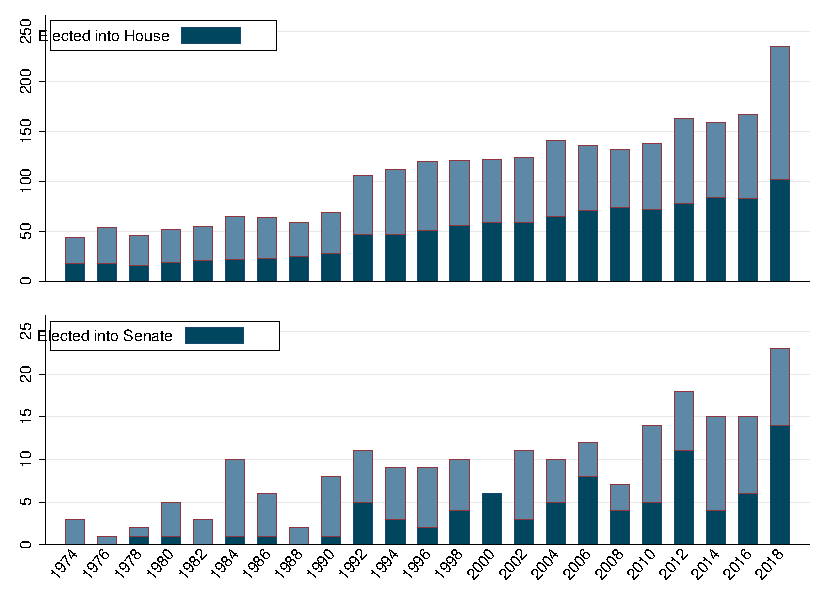
\includegraphics[width=0.65\linewidth]{figures/cawp.pdf}\vspace{-1.5em}
	\caption{
		Women in Congress.\\
		\emph{Note:}
		The figure shows the number of women elected to the US House of Representatives (top panel) and the US Senate (bottom panel) from 1974 to 2018.
		The dark-shaded portions represent successful elections.
		Data is from the Center for American Women and Politics \citep{cawp}.
	}
	\label{fig:cawp} 
\end{figure}

The link between the MeToo movement and the 2018 election may also stem from candidate choices.
Women were historically underrepresented in politics \citep[e.g.,][]{thomsen2020, cawp}.
The 2018 elections, however, subverted this trend through a historic level of representation from women candidates (\cref{fig:cawp}).
Districts with a stronger movement might unconditionally spur more women challengers, but in reality, candidacy emergence also depends critically on the strategic calculus within party politics.
In particular, incumbent partisanship shapes these decisions in distinct ways for cross-partisan versus co-partisan challenges.

Cross-partisan challenges represent standard electoral competition.
Opposition parties regularly challenge incumbents, and candidate gender may be secondary to other factors determining same-party competition for the party's nomination.
For Democratic women challenging Republican male incumbents in 2018, the movement could have provided multiple advantages, such as the heightened salience of gender issues and a national narrative around women as agents of (legal) change \citep{Tippett2018, tippett2018-bi, nyt2018} (\cref{sm:legal}).
If true, cross-partisan challenges by Democratic women would be more likely in districts with more intense MeToo activity.
On the other hand, the Republican Party, with its smaller pool of women candidates \citep{thomsen2020} and lower solidarity with the movement \citep{dittmar2020}, is unlikely to respond in similar ways.

Same-party challenges usually face strong informal constraints, with party norms discouraging primary challenges to co-partisan incumbents.
The statistical evidence suggests that in districts where the movement is stronger, these norms appear weaker, and co-partisan challenges are more easily framed as politically legitimate.
For Democratic women, MeToo could have legitimized challenges to co-partisan male incumbents by framing such challenges as necessary for the party to credibly address gender issues and sexual misconduct.
To this extent, norm disruption within the Democratic party might be stronger in districts where MeToo activity had more traction.

%===============================================================================
\subsection{Estimation}
\label{sec:candidacy-estimation}
To test whether the MeToo movement shaped women candidacy,  I model the probability of having a woman challenger as a function of district-level movement strength and incumbent characteristics:
%%%%%%%%%%%%%%%%%%%%%%%%%%%%%%%% EQUATION %%%%%%%%%%%%%%%%%%%%%%%%%%%%%%%%%%%%%%
\begin{equation}
\label{eq:candidacy}
\text{WomanChallenger}_{d}^{(\text{party})} = 
\alpha_1 \tau_d + 
\alpha_2 \theta_d + 
\beta (\tau \times \theta)_d + 
\bm{\Gamma} \bm{X}_d + 
\text{State}_{s(d)} + 
\varepsilon_{d},
\end{equation}
%%%%%%%%%%%%%%%%%%%%%%%%%%%%%%%% EQUATION %%%%%%%%%%%%%%%%%%%%%%%%%%%%%%%%%%%%%%
where $\tau_d$ is the district-level log tweet density (mean-centered),
$\theta_d$ indicates incumbent type (Republican man or Democratic man), 
$\bm{X}_d$ include demographics and past electoral trends (\cref{sec:voteshare-estimation}).
$\tau_d$ is mean-centered so that $\alpha_2$ captures how women candidacy responds to incumbent type at mean levels of the movement.
$\alpha_1$ captures whether women candidacy responds unconditionally to the movement.
The key parameter of interest is the interaction coefficient $\beta$, which captures whether the association between women candidacy and incumbent partisanship differs by the level of the movement.
As complementary visualizations, I also estimate the marginal effects of the Metoo movement on candidacy using kernel smoothing for flexible functional forms of the interaction term \citep{interflex}.
I estimate \cref{eq:candidacy} separately for Republican and Democratic women challengers, and for each, I run two specifications examining Republican male incumbents and Democratic male incumbents as the moderating variable $\theta_d$ to examine co-partisan and cross-partisan behavior.
All regressions include state-fixed effects ($\text{State}_{s(d)}$), with standard errors clustered by state.

%===============================================================================
\subsection{Results}
\label{sec:candidacy-results}

\begin{table}[tbp]
	\centering
	\setlength\tabcolsep{8 pt} 
	\setlength{\defaultaddspace}{0pt}
	\def\sym#1{\ifmmode^{#1}\else\(^{#1}\)\fi}
	\caption{MeToo Movement and Candidacy as Strategic Reaction}
	\label{tab:candidacy}
	\begin{adjustbox}{max width=1\textwidth}
		\begin{tabular}{@{\hspace{0\tabcolsep}}l*{4}{D{.}{.}{-1}}@{\hspace{0\tabcolsep}}}
			\toprule\toprule
			&\multicolumn{4}{c}{Outcome is women challenger from the}\\
			\cmidrule{2-5}
			&\multicolumn{2}{c}{Republican party}&\multicolumn{2}{c}{Democratic party}\\
			\cmidrule(r){2-3} \cmidrule(l){4-5}
			&\multicolumn{1}{c}{(1)}&\multicolumn{1}{c}{(2)}&\multicolumn{1}{c}{(3)}&\multicolumn{1}{c}{(4)}\\
			\midrule
			Log tweet density   &   0.038         &   0.016         &  -0.089         &  -0.086         \\
                    & (0.049)         & (0.042)         & (0.056)         & (0.058)         \\
Republican man incumbent&  -0.136\sym{***}&                 &   0.226\sym{***}&                 \\
                    & (0.037)         &                 & (0.059)         &                 \\
Democratic man incumbent&                 &   0.019         &                 &  -0.417\sym{***}\\
                    &                 & (0.032)         &                 & (0.055)         \\
Log tweet density $ \times $ (Republican man incumbent)&  -0.033         &                 &   0.097         &                 \\
                    & (0.038)         &                 & (0.075)         &                 \\
Log tweet density $ \times $ (Democratic man incumbent)&                 &  -0.009         &                 &   0.162\sym{***}\\
                    &                 & (0.097)         &                 & (0.049)         \\
State fixed effects &\multicolumn{1}{c}{$ X $}         &\multicolumn{1}{c}{$ X $}         &\multicolumn{1}{c}{$ X $}         &\multicolumn{1}{c}{$ X $}         \\
Census Control      &\multicolumn{1}{c}{$ X $}         &\multicolumn{1}{c}{$ X $}         &\multicolumn{1}{c}{$ X $}         &\multicolumn{1}{c}{$ X $}         \\
F-test: Electoral controls = 0&\multicolumn{1}{c}{$ F = 4.65^{**} $}         &\multicolumn{1}{c}{$ F = 3.18^{**} $}         &\multicolumn{1}{c}{$ F = 1.95 $}         &\multicolumn{1}{c}{$ F = 1.24 $}         \\
F-test: County census = 0&\multicolumn{1}{c}{$ F = 2.46^{**} $}         &\multicolumn{1}{c}{$ F = 3.45^{**} $}         &\multicolumn{1}{c}{$ F = 2.76^{**} $}         &\multicolumn{1}{c}{$ F = 2.79^{**} $}         \\
$ R^2 $             &   0.218         &   0.189         &   0.230         &   0.296         \\
$ N $               &\multicolumn{1}{c}{$ 382 $}         &\multicolumn{1}{c}{$ 382 $}         &\multicolumn{1}{c}{$ 382 $}         &\multicolumn{1}{c}{$ 382 $}         \\
			\bottomrule
		\end{tabular}
	\end{adjustbox}
	\caption*{
		\footnotesize
		\emph{Notes:}
		The dependent variable is an indicator for the presence of a woman challenger from each party in the district.
		Estimates are from linear probability models (\cref{eq:candidacy}).
		The log tweet density measure is mean-centered.
		Columns (1)--(2) examine Republican women challengers; columns (3)--(4) examine Democratic women challengers.
		Odd-numbered columns condition on Republican male incumbency; even-numbered columns condition on Democratic male incumbency.
		Robust standard errors clustered by state.
		Significance levels: $^*$ 0.1 $^{**}$ 0.05 $^{***}$ 0.01.
	}
\end{table}

\cref{tab:candidacy} presents estimates examining how male incumbent partisanship moderates the relationship between district-level MeToo activity and women candidacy.

Columns (1)--(2) examine the emergence of Republican women challengers.
At mean levels of movement activity, Republican women are significantly less likely to challenge Republican male incumbents ($\hat{\beta} = -0.14$, $p < .01$), consistent with party norms discouraging co-partisan challenges.
The interaction between MeToo activity and Republican male incumbency is not statistically significant ($\hat{\beta} = -0.03$, $p > .1$), suggesting these norms persist in districts with a strong MeToo movement.
Column (2) shows that Democratic male incumbents do not predict Republican women challengers, either as a main effect or through moderation by the movement.

Columns (3)--(4) shift to Democratic women challengers.
Column (3) reveals that at mean levels of MeToo activity, Democratic women are significantly more likely to challenge in districts with a Republican male incumbent ($\hat{\beta} = 0.23$, $p < .01$).
However, the interaction term is not statistically significant ($\hat{\beta} = 0.10$, $p > .1$), indicating this cross-partisan pattern exists independent of the MeToo movement.

Finally, Column (4) reveals striking patterns for Democratic co-partisan challenges.
At mean movement levels, Democratic women are significantly less likely to challenge Democratic male incumbents ($\hat{\beta} = -0.42$, $p < .01$), again, reflecting party norms discouraging co-partisan challenges.
Critically, however, the interaction between MeToo activity and Democratic male incumbency is positive and highly significant ($\hat{\beta} = 0.16$, $p < .01$).
The estimate implies that a one SD increase in MeToo activity predicts a 14 percentage point increase in the probability of a Democratic woman challenging a co-partisan male incumbent.

\begin{figure}[tbp]
	\centering
	\begin{subfigure}{.495\textwidth}\centering
		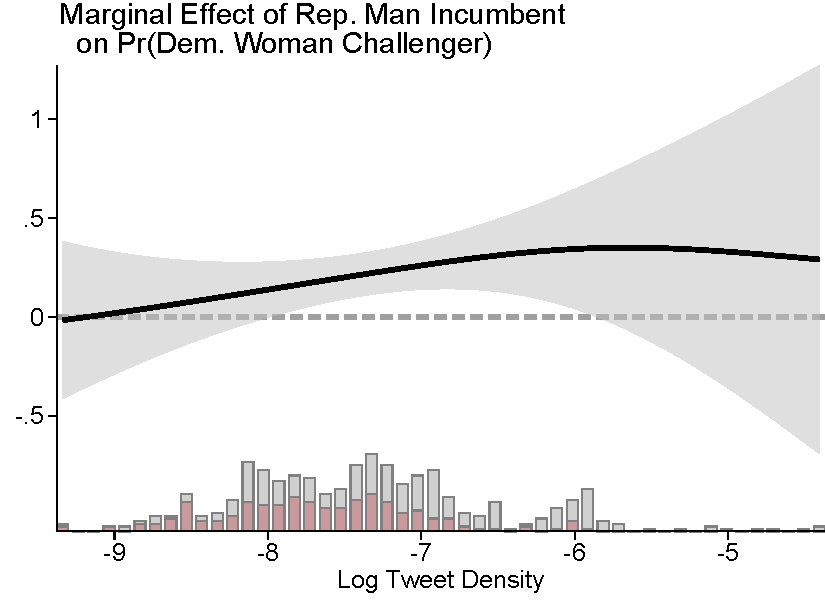
\includegraphics[width=\textwidth]{figures/atLeast1DemWomanChallenger-repManIncumbent.pdf}
		\caption{Conditional on Republican Male Incumbents}
	\end{subfigure}
	\hfill
	\begin{subfigure}{.495\textwidth}\centering
		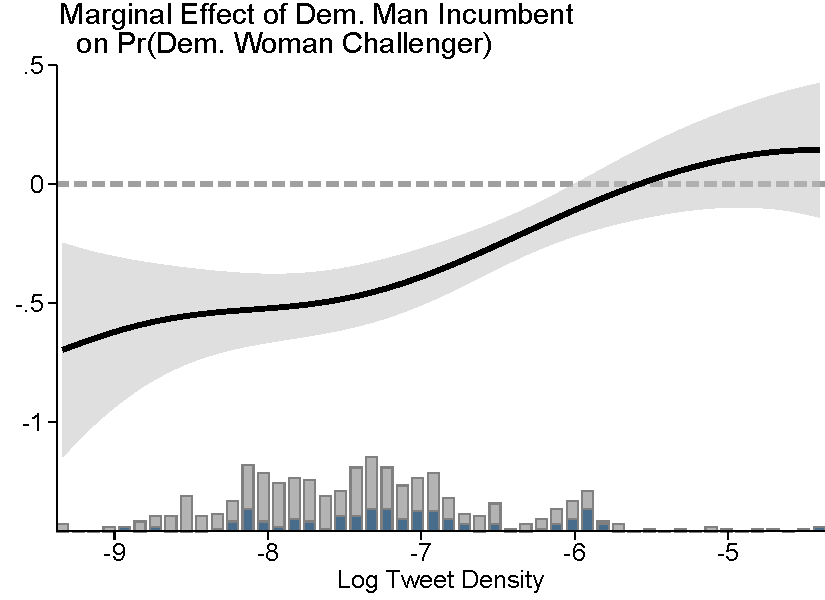
\includegraphics[width=\textwidth]{figures/atLeast1DemWomanChallenger-demManIncumbent.pdf}
		\caption{Conditional on Democratic Male Incumbents}
	\end{subfigure} 
	\vspace{-.8em} 
	\caption{
		Democratic Women Candidacy as Strategic Reaction.\\
		\emph{Note:}
		This figure reports the marginal effects of male incumbent partisanship on the probability of a Democratic woman challenger, moderated by the MeToo movement (log tweet density).
		Estimates correspond with Columns (3)--(4) of \cref{tab:candidacy}: Left panel with Column (3); Right panel with Column (4).
		Histograms report the distribution of the log tweet density by incumbency type.
	}
	\label{fig:interflex}
\end{figure}

\cref{fig:interflex} visualizes these effects from Column (4) of \cref{tab:candidacy}.
At low levels of the movement, Democratic women are significantly less likely to challenge co-partisan male incumbents (the marginal effect is negative).
However, at higher levels of the movement, this relationship approaches zero, implying a neutralization of norms against co-partisan challenges.

Analyses using the 2016 election data (\cref{sm:2016-elections}) confirm that the Democratic co-partisan norm disruption is distinctive to 2018, while confirming the baseline intra-party norm that discourages co-partisan challenges (\cref{tab:candidacy-2016}).

%===============================================================================
\subsection{Strategic Candidacy as Mechanism}
These findings reveal that the MeToo movement shaped both inter-party and intra-party competition for women candidates, but in asymmetric ways.
First, the estimates confirm intra-party norms for both parties, where women are less likely to stand in districts where the incumbent is a co-partisan male.
However, the results suggest that these norms weaken for the Democratic party, in that strong movement increases the probability of women candidates in districts held by co-partisan men.
This pattern does not extend to the Republican party, consistent with their difficulty fielding quality women candidates \citep{thomsen2020, CarsonHitefield2018} and lower solidarity with the movement \citep{dittmar2020}.%
\footnote{While half of the Democratic women challengers expressed solidarity with the movement, only one in five from the Republican party did so \citep{dittmar2020}.}

Six Democratic women won seats against co-partisan male incumbents.
In particular, one in a seat vacated after sexual misconduct allegations \citep{nyt2018}.
Four are members of the left-leaning group, ``The Squad''.
The remaining two won in safe \D{} Texas districts.
All six succeeded in districts that are pronouncedly \D{}, consistent with an absence of credible evidence that the movement had direct electoral benefits for Democratic vote share (\cref{sec:voteshare-results}).
In contrast, 17 Democratic women flipped Republican-held seats, including notable upsets like Kendra Horn in Oklahoma's R+10 5th district and Lizzie Fletcher in Texas's R+7 7th district.
These cross-partisan victories likely constituted the primary driver of Democratic gains in 2018, but the candidacy results (\cref{sec:candidacy-results}) suggest such cross-party challenges did not vary with the local movement levels.

The political profile of these Democratic women candidates resembled those in 2016 \citep{thomsen2020}, suggesting demand-side factors fueled by the movement rather than a fundamental reshaping of the gendered pipeline to power \citep{Safarpour2022, CarsonHitefield2018, Lucas2021, dittmar2020, DeMora2023, Gibson2019, thomsen2020}.
Many were lawyers \citep{thomsen2020}, reflecting public sentiment that representational shifts in Congress are necessary for substantive legislative change (\cref{sm:legal}).
Overall, the results suggest that a key mechanism was candidate selection.
Quality Democratic women candidates \citep{CarsonHitefield2018} responded strategically to constituency demands amplified through social media \citep{wholeads2019}.

%-------------------------------------------------------------------------------
%-------------------------------------------------------------------------------
\section{Turnout}
\label{sec:turnout}
%-------------------------------------------------------------------------------
%-------------------------------------------------------------------------------
A final mechanism I examine is voter turnout.
Midterm elections generally have a different electoral environment than those in presidential years, with lower turnouts \citep{Lucas2021}.
Yet, the 2018 elections saw historically high turnout, with some estimates exceeding 53\% \citep{brookings2019turnout}.
The MeToo movement is thus hypothesized to have played a part by centering gender and political accountability in 2018, turning the midterms into uncharacteristically nationalized and president-centered elections \citep[\cref{sec:background};][]{Lucas2021, womenmarch, CarsonHitefield2018, Safarpour2022, genderwatch2018, telegraphMetoo, tippett2018-bi, thomsen2020}.

One possibility is that MeToo discourse mobilized voters in areas where its message about political accountability and gender dynamics resonated most strongly.
Since social movements can spur participation by increasing issue salience and creating opportunities for political engagement \citep{McAdam_Tarrow_2010}, this predicts higher turnout in counties with stronger MeToo activity. 

Alternatively, mobilization effects might have been strongest in Republican-leaning areas.
In Democratic counties, the marginal gains from a strong local MeToo movement would be limited.
In Republican-leaning counties, however, the anti-Trump sentiment of the movement (\cref{sec:background}) may have mobilized left-leaning voters who might have otherwise stayed home if they perceived the movement as signaling possibilities for political change even in unfavorable territory.
This predicts that MeToo activity should increase turnout more in counties with higher Trump support in 2016.

To test these theories, I examine whether county-level tweet density predicts turnout increases from 2016 to 2018, and whether Trump's 2016 vote share moderated it.
In addition, given the concern about comparing a presidential election year (2016) to a midterm year (2018), I also examine changes from 2014 to 2018 to compare across midterm elections.

%===============================================================================
\subsection{Estimation}
\label{sec:turnout-estimation}
To test whether the MeToo movement predicts changes in voter turnout, I model the change in total votes cast in county $c$ as:
\begin{equation}
\label{eq:turnout}
\Delta\text{turnout}_c^{2016\text{--}2018} = 
\alpha_1 \tau_c + 
\alpha_2 \nu^{\text{Rep., Pres.}}_{c,\ 2016} + 
\beta (\tau \cdot \nu^{\text{Rep., Pres.}})_c + 
\bm{\Gamma} \bm{X}_c + 
\text{State}_{s(c)} +
\varepsilon_c,
\end{equation}
where $\Delta\text{turnout}_c^{2016\text{--}2018} = \ln(\text{votes}_{c,2018}) - \ln(\text{votes}_{c,2016})$ captures the percentage change in total House votes cast.
$\alpha_1$ measures the association between tweet density ($\tau_c$) and turnout change, and $\beta$ captures whether it varies with Trump's 2016 presidential vote share ($\nu^{\text{Rep., Pres.}}_{c,\ 2016}$).
Demographic controls ($\bm{X}_c$) are both levels and trends using the ACS 5-year estimates from 2012--16 and 2015--19, which include the population and civilian voting-aged electorate in log terms.%
\footnote{The exception is the percentage of rural population, available only from the decennial census.}
Additional controls include turnout in the 2016 presidential and House elections, the 2012 presidential Republican vote share, and state fixed effects.
Standard errors are clustered by state.
I also estimate \cref{eq:turnout} using the 2014 turnout to compare midterm-to-midterm election changes ($\Delta\text{turnout}_c^{2014\text{--}2018}$).

%===============================================================================
\subsection{Results}
\label{sec:turnout-results}

\begin{table}[tbp]
	\centering \small \setlength\tabcolsep{2 pt} \setlength{\defaultaddspace}{0pt}
	\def\sym#1{\ifmmode^{#1}\else\(^{#1}\)\fi}
	\caption{MeToo Movement and the Change in Voter Turnout}
	\label{tab:turnout}
	\begin{adjustbox}{max width=1\textwidth}
		\begin{tabular}{@{\hspace{0\tabcolsep}}l*{4}{D{.}{.}{-1}}@{\hspace{0\tabcolsep}}}
			\toprule\toprule
			&\multicolumn{4}{c}{Outcome is change in voter turnout}\\
			\cmidrule{2-5}
			&\multicolumn{2}{c}{2016--2018 change}&\multicolumn{2}{c}{2014--2018 change}\\
			\cmidrule(r){2-3} \cmidrule(l){4-5}
			&\multicolumn{1}{c}{(1)}&\multicolumn{1}{c}{(2)}&\multicolumn{1}{c}{(3)}&\multicolumn{1}{c}{(4)}\\
			\midrule
			Log tweet density   &  0.0184         &  0.0181         &  0.0178         &  0.0189         \\
                    &(0.0164)         &(0.0179)         &(0.0163)         &(0.0173)         \\
Pres. 2016 Republican vote share& -0.0009         & -0.0007         & -0.0036\sym{**} & -0.0042\sym{**} \\
                    &(0.0044)         &(0.0054)         &(0.0015)         &(0.0021)         \\
Log tweet density $ \times $ (Pres. 2016 Republican vote share)&                 &  0.0000         &                 & -0.0001         \\
                    &                 &(0.0003)         &                 &(0.0003)         \\
State fixed effects&\multicolumn{1}{c}{$ X $}         &\multicolumn{1}{c}{$ X $}         &\multicolumn{1}{c}{$ X $}         &\multicolumn{1}{c}{$ X $}         \\
Census Control      &\multicolumn{1}{c}{$ X $}         &\multicolumn{1}{c}{$ X $}         &\multicolumn{1}{c}{$ X $}         &\multicolumn{1}{c}{$ X $}         \\
F-test: Electoral controls = 0&\multicolumn{1}{c}{$ F = 2.4^{*} $}         &\multicolumn{1}{c}{$ F = 1.85 $}         &\multicolumn{1}{c}{$ F = 3.45^{**} $}         &\multicolumn{1}{c}{$ F = 3.85^{**} $}         \\
F-test: County census = 0&\multicolumn{1}{c}{$ F = 1.44 $}         &\multicolumn{1}{c}{$ F = 1.46 $}         &\multicolumn{1}{c}{$ F = 10.47^{***} $}         &\multicolumn{1}{c}{$ F = 10.64^{***} $}         \\
$ R^2 $             &  0.3719         &  0.3719         &  0.4255         &  0.4255         \\
$ N $               &\multicolumn{1}{c}{$ 3101 $}         &\multicolumn{1}{c}{$ 3101 $}         &\multicolumn{1}{c}{$ 3097 $}         &\multicolumn{1}{c}{$ 3097 $}         \\
			\bottomrule
		\end{tabular}
	\end{adjustbox}
	\caption*{
		\footnotesize
		\emph{Notes:}
		Observations are at the county level.
		The dependent variable is the log of total county votes cast in the 2018 House elections minus the same variable for the 2016 (columns (1)--(2)) or the 2014 (columns (3)--(4)) House elections.
		The Republican presidential vote share is centered at 50\%.
		County census controls include the 14 demographic variables and additionally the percentage of citizen voting-age population; these are entered as both levels and changes from the ACS 5-year estimates for 2012--16 and the ACS 5-year estimates for 2015--19, except for the percentage rural population, available only from the decennial census.
		Robust standard errors in parentheses are clustered by state.
		Significance levels: $^*$ 0.1 $^{**}$ 0.05 $^{***}$ 0.01.
	}
\end{table}

\cref{tab:turnout} reports the turnout results.
The estimate for tweet density is positive ($0.0184$, $p > .1$), implying that a one SD increase in tweet density is associated with a 2.1\% increase in turnout, a sizeable but statistically insignificant association.
% SD of log tweet density = 1.164888
% Calculation: 0.0184 * 1.164888 = 0.0214 ≈ 2.1%
In particular, the interaction effect is effectively zero ($\hat{\beta}=0.00003$, $p > .1$), implying that for a SD increase in the MeToo measure, every ten percentage point increase in the Republican vote share is associated with only a 0.03\% increase in turnout, although not statistically significant.
% SD of log tweet density = 1.164888
% Calculation: 0.00003 * 1.164888 * 10 = 0.00035 ≈ 0.03%
A concern is that comparing 2016 to 2018 might conflate secular turnout behavior with the social movement, since that compares a presidential election year to the midterms.
Columns (3)--(4) examine the change in turnout from the 2014 to 2018 midterm years, with similarly null findings.

%===============================================================================
\subsection{Interpretation}
\label{sec:turnout-discussion}
Overall, the results on voter turnout show no connection between the MeToo tweet density and changes in turnout from 2016 to 2018 or from 2014 to 2018.

The 2018 midterms nevertheless saw historically high turnout \citep{census2019turnout, brookings2019turnout, GalstonHendrickson2019}.
From census estimates, this surge appeared to be driven by multiple factors, including young voters, ethnic-minority voters, and shifting demographics among college-educated whites \citep{brookings2019turnout, census2019turnout}.
Moreover, gender gaps in turnout were particularly pronounced among younger voters \citep{census2019turnout}.
Collectively, these demographic and political dynamics are consistent with MeToo's broader suggested social movement, and in this sense, the movement may have played a part in mobilizing voters during the 2018 elections.
However, the data show no such associations.

This null finding stands in contrast to some studies of media, protests, and political mobilization:
Fox News increased turnout (and Republican votes) in 2000 \citep{DellaVigna2007}, online activism fueled Italy's Five Star Movement in 2009, mobilizing many first-time voters \citep{Campante2017}, and in the UK, the 2011 London riots raised political awareness and increased voter turnout \citep{leon2022}.
The lack of a detectable turnout effect in this study suggests that any effect of the MeToo movement on voter mobilization was more likely driven by national political dynamics than by localized movement activity.

%-------------------------------------------------------------------------------
%-------------------------------------------------------------------------------
\section{Conclusion}
\label{sec:conclusion}
%-------------------------------------------------------------------------------
%-------------------------------------------------------------------------------
This study examines whether and how decentralized social media activism shapes electoral outcomes, through the MeToo movement and the 2018 midterm House elections.
To measure the local strength of the movement, I geocode ``\#metoo'' tweets in 2018 and measure county-level variation by population-normalizing the measures.
A critical challenge is establishing whether these large-scale digital traces reflect authentic narratives of the social movement, which I address through multiple approaches.
First, the semantic topic modeling and network analyses confirm substantive engagement with movement themes and figures, as do analyses of hashtag co-occurrences and named entity recognition.
Moreover, linking the county-level measure to micro survey data reveals that the strength of the local movement predicts disapproval of the Republican party in the handling of sexual harassment issues, and predicts general individual-level attitudes to sexism.

The econometric analysis exploits within-district geographic variation, revealing an apparent Democratic advantage in vote shares in Republican counties that had strong movement activity.
However, I use the 2016 returns as falsification tests and find similar patterns, suggesting that the direct benefits reflect pre-existing demographic trends rather than the true effects of the movement.
Comparing turnout changes from 2014 to 2016 and 2016 to 2018 likewise reveals no movement-driven differences.
Instead, consistent with a historic level of women representation, the movement appeared to operate through strategic women candidacy, where women were significantly more likely to rise against co-partisan male incumbents, a pattern absent in the 2016 elections.
Fundamentally, the results challenge simple narratives about ``\#MeToo elections'' by revealing that movement alone does not determine electoral impact.

\subsection{Limitations}
The text analyses of the sample \#metoo tweets, including topic modeling, named entity recognition, and network analysis, provide descriptive evidence of substantive engagement with the movement's discourse.
Moreover, analyses using the VOTER survey demonstrate that the \#metoo tweet measure captures the geographical distribution of individual-level attitudes on issues of sexual harassment and political accountability.
Nonetheless, these checks do not definitively establish that the sampled tweets originate from representative residents.

The county-level variation of the MeToo movement is less sensitive to political border shifts and helps address unobserved confounders at the congressional district level \citep[e.g.,]{cs, womenmarch, DellaVigna2007}, but has limitations.
First, counties coterminous with their district do not contribute to the estimation, making results dependent on multi-county districts, which limits generalizability.
Similarly, districts with few counties contribute little to estimation.
Second, county and district borders evolve differently.
Districts are redrawn based on population, while county lines are largely static.
Combined with growing urbanization, this implies that suburban and rural districts are geographically large and tend to contain many counties, while urban districts do not.%
\footnote{Districts are apportioned by population size every ten years, according to the US Constitution. However, county borders are more idiosyncratic, infrequently adjusted, and more determined by historic episodes such as the colonial land grant era than contemporary population size.}
This skews the measured association of the MeToo movement towards rural, white, and traditionally Republican areas.
Relatedly, while models for changes in turnout adjust for demographic shifts, they may not fully capture underlying trends related to cross-county migration or younger voters coming of age.

Lastly, this study examines only House elections, as only a third of Senate seats were contested in 2018.
Nonetheless, the House plays a critical role in national legislation, including initiating presidential impeachment, and, keeping with the theme of the grassroots, is more responsive to their constituencies \citep[e.g.,][]{wholeads2019}.

\subsection{Social Movements and Electoral Outcomes}
The MeToo movement catalyzed into public conversation on social media (Twitter) in 2018 \citep{goenaga2021}, leading to widespread expectations of congressional change through Democratic gains in the midterm elections \citep{genderwatch2018, telegraphMetoo, thomsen2020, tippett2018-bi}.
On the contrary, I find no credible evidence that the movement increased Democratic vote shares or turnout.
These null findings echo broader research questioning whether social media activism translates into electoral persuasion \citep{cs}.

Instead, the most credible signal lies in women's candidacy.
The evidence suggests that the movement propelled a subset of non-incumbent Democratic women candidates to disrupt traditional party norms by challenging their co-partisan male incumbents, enabling them to frame their rise as ideologically principled responses to their constituencies \citep{wholeads2019} rather than violations of party norms.
While the analyses of the tweet content confirm that the MeToo discourse is closely connected to anti-Trump opposition, the findings do not suggest any effect from the movement as a general anti-Trump referendum.
Instead, the evidence points to a higher demand for women candidates, a call answered from within the Democratic Party.

However, it is unclear whether such findings would generalize.
Many successful challenges came from quality candidates, many of whom were lawyers \citep{thomsen2020}, reflecting public sentiment that demographic shifts in Congress were necessary.
But their professional backgrounds resembled their predecessors in 2016, suggesting no fundamental reshaping of the gendered pipeline to power \citep{thomsen2020}.
More likely is the case that these were pre-existing but strategically positioned candidates who could credibly claim alignment with the movement, thereby legitimizing their within-party rise.
Without such political happenstance, such effects are unlikely to replicate in other elections.

%TC:ignore
\begin{acks}
I am grateful to Wai Mun Chia, Shubhankar Dam, Yohanes Eko Riyanto, Chris Sakellariou, Gaurav Sood, You Yenn Teo, and Walter Edgar Theseira for their detailed comments. I also thank Chris Youderian for clarifying how the USGS defines the primary U.S. counties. To~Giovanni~Ko.
\end{acks}

\bibliographystyle{ACM-Reference-Format}
\bibliography{references}

\clearpage
\appendix

\vspace{1cm}
\noindent \textbf{Supplementary Information}\\
\hyperref[sm:data]{\indent \textcolor{magenta}{\S A.}} Data Appendix\\
\hyperref[sm:text]{\indent \textcolor{magenta}{\S B.}} MeToo Tweet Content\\
\hyperref[sm:random-samples]{\indent \textcolor{magenta}{\S C.}} MeToo Tweet Samples\\
\hyperref[sm:VOTER]{\indent \textcolor{magenta}{\S D.}} VOTER Individual-Level Attitudes and Voting Behavior\\
\hyperref[sm:legal]{\indent \textcolor{magenta}{\S E.}} Legal Implications of MeToo\\
\hyperref[sm:2016-elections]{\indent \textcolor{magenta}{\S F.}} Back to the 2016 Elections\\
\hyperref[sm:density-intensity]{\indent \textcolor{magenta}{\S G.}} Density vs. Intensity\\

\FloatBarrier
\setcounter{table}{0}
\setcounter{figure}{0}
\setcounter{equation}{0}
\renewcommand{\thetable}{A\arabic{table}}
\renewcommand{\thefigure}{A\arabic{figure}}
\renewcommand{\theequation}{A\arabic{equation}}

\begin{bibunit}
\makeatletter
\let\appx@natlinkstart\hyper@natlinkstart
\def\hyper@natlinkstart#1{\appx@natlinkstart{appx.#1}}
\let\appx@natanchorstart\hyper@natanchorstart
\def\hyper@natanchorstart#1{\appx@natanchorstart{appx.#1}}
\makeatother

%-------------------------------------------------------------------------------
\section{Data Appendix}
\label{sm:data}
%-------------------------------------------------------------------------------
\small
To download and map the tweets to counties, I proceed as follows:
\begin{enumerate}
	\item{I use the \textit{GetOldTweets-python} pseudo-API by Jefferson Henrique (\url{https://github.com/Jefferson-Henrique/GetOldTweets-python}), which scrapes the Twitter Search browser for tweets containing the MeToo hashtag.
	The Official Twitter API has a 7-day limit on past tweets at the time of this writing, which this library circumvents. Under the hood, the third-party API scrapes Twitter Search, enabling users to find historical tweets containing specific keywords. Search results appear in a scroll loader that loads more tweets via calls to a JSON provider as a user continues scrolling, without a definite limit. At the time of use, I need to make changes to two lines of the code to retrieve the author's username, as noted in the \emph{issues} of the repository. }
	
	\item{With the usernames, I query the Official Twitter API, which returns their user geolocation strings. 
		Of the 700,891 usernames, 158,857 cannot be found via the Twitter API at the time of the query, and another 21,521 users are found but the geolocation string is left empty.
		For the remaining 520,513, I obtained the geolocation data for the Twitter accounts.}
	
	\item{I use a series of hard-coded rules to parse the various user-input geolocations into a standardized US city-state format (e.g., Philadelphia, Pennsylvania). I first retain only ASCII characters in a string, removing non-English symbols. After retaining only ASCII characters, 87,123 geolocation strings are 7 characters or fewer, indicating that a sizable number of Twitter users enter non-ASCII characters.}
	
	\item{I then check whether the geolocation string can be unambiguously identified as a non-US country. If so, these are filtered out immediately. Using the ISO-3166 country names and codes, 89,115 (17\% of 520,513) of the geolocation strings are immediately identified as Twitter users who list a non-US country as their location.}
	
	\item{For the remaining geolocation strings, I check if they can be identified as a US city-state by searching for both state names and postal codes, as well as city names within the string. \cref{al:parse-geoloc} provides the specific hard-coded rules used. \cref{tab:examples-parseGeoLoc} provides some examples. The rules allow me to successfully parse 130,433 (25\% of 520,513) geolocations into a standard US city-state format. A relatively small percentage of geolocation strings, 19,590 or 3.8\%, is stated as the United States but omits information about the state, the city, or both.}
	
	\item{
		To filter out automated accounts, I use Botometer X, developed by Indiana University's Observatory on Social Media.
		The tool is based on an ensemble of Random Forest classifiers trained on labeled human and bot accounts, producing scores between 0 (likely human) and 1 (likely bot) \citep{botometer101} (\url{https://botometer.osome.iu.edu/faq}).
		I query Botometer X for the user ID of the 130,433 unique geocoded accounts.
		The majority of accounts have low scores, indicating that they likely reflect organic social media content (see \cref{fig:botometer_score_distribution} for the distribution of scores). 
		I retain those with scores below 0.5, resulting in 121{,}878 (93.4\%) geocoded accounts that are inferred as likely human accounts.
	}
	
	\item{Finally, I match the tweets by US city-states to their primary counties (\cref{fig:choropleth-tweets}) using the \textit{United States Cities Database} (\url{https://simplemaps.com/data/us-cities}). The primary counties are defined by the US Geological Survey, which takes the centroid of a city and then records the county in which the centroid lies.}
\end{enumerate}
\input{tables/parse-geoloc.txt}

\begin{figure}[!h]
	\centering
	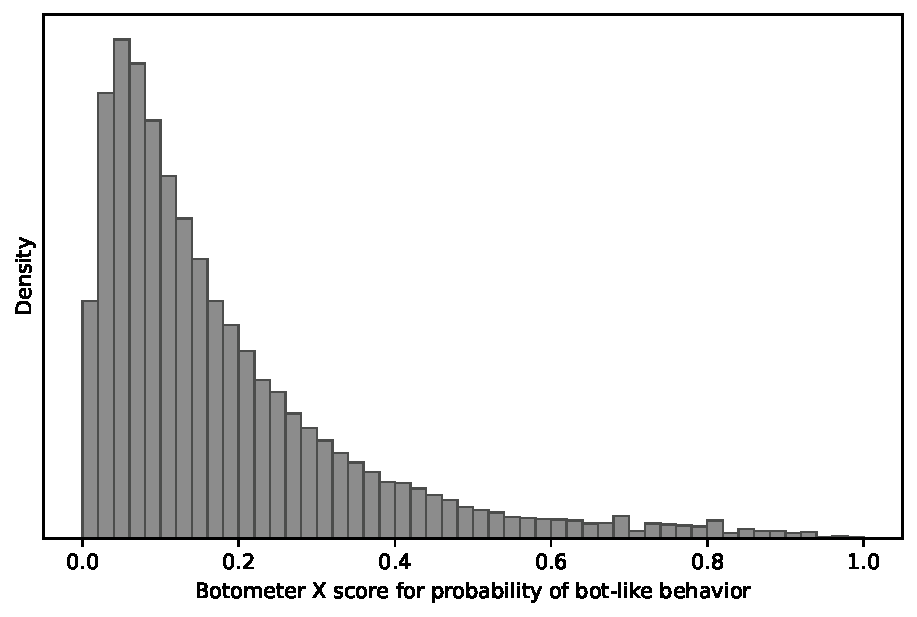
\includegraphics[width=.65\linewidth]{figures/botometer_score_distribution.pdf}
	\caption{
		\textsc{Sample distribution of Botometer X probability scores ($n = 130{,}433$).}
		Higher scores indicate higher probability of bot-like behavior.
	}
	\label{fig:botometer_score_distribution}
\end{figure}

\normalsize

\begin{table}[ht]
	\centering \scriptsize \setlength\tabcolsep{2 pt}
	\caption{Examples of Parsing Twitter User Geolocation}
	\label{tab:examples-parseGeoLoc}
	\begin{adjustbox}{max width=\textwidth}
		\begin{tabular}{@{\hspace{0\tabcolsep}}lll|@{\hspace{3\tabcolsep}}lll@{\hspace{0\tabcolsep}}}
			\toprule\toprule
			User Geolocation                                      & State                & (Primary) County & User Geolocation                                      & State                & (Primary) County     \\
			\midrule
			nomadic & --- & --- & sandy oaks, tx & Texas & Bexar \\
			los angeles, ca & California & Los Angeles & calcinato, lombardia & --- & --- \\
			pensacola, fl & Florida & Escambia & london, england & --- & --- \\
			victoria, bc, canada & --- & --- & virginia & --- & --- \\
			washington, dc & District of Columbia & District Of Columbia & dallas, tx & Texas & Dallas \\
			south ca & --- & --- & united states & --- & --- \\
			michigan, usa & --- & --- & bordeaux, aquitaine & --- & --- \\
			oxford, ms & Mississippi & Lafayette & chicago & Illinois & Cook \\
			port townsend, wa & Washington & Jefferson & ut & --- & --- \\
			namak haram in pakistan & --- & --- & lagos, nigeria & --- & --- \\
			boston, ma & Massachusetts & Suffolk & grittydelphia via la,nyc,gb & --- & --- \\
			pakistan & --- & --- & oakland, ca & California & Alameda \\
			united states & --- & --- & st louis, mo & Missouri & St. Louis (City) \\
			kitchener, ontario & --- & --- & san francisco, ca & California & San Francisco \\
			stanford, ca & California & Santa Clara & probably on the floor sumwhere & --- & --- \\
			chicago, il & Illinois & Cook & houston, tx & Texas & Harris \\
			micromsmemumbaiwala & --- & --- & mother earth & --- & --- \\
			houston, tx & Texas & Harris & cleveland, tn & Tennessee & Bradley \\
			oregon, usa & --- & --- & tuscaloosa & Alabama & Tuscaloosa \\
			new york & New York & New York & provo, ut & Utah & Utah \\
			united states & --- & --- & grand rapids, mi & Michigan & Kent \\
			the village & Oklahoma & Oklahoma & san francisco & California & San Francisco \\
			murcia, espana & --- & --- & mount greenwood, chicago & --- & --- \\
			morgantown, wv & West Virginia & Monongalia & las vegas, nv & Nevada & Clark \\
			new jersey, usa & --- & --- & whalley, bc & --- & --- \\
			\bottomrule
		\end{tabular}
	\end{adjustbox}
\end{table}

\begin{figure}[ht]
	\centering
	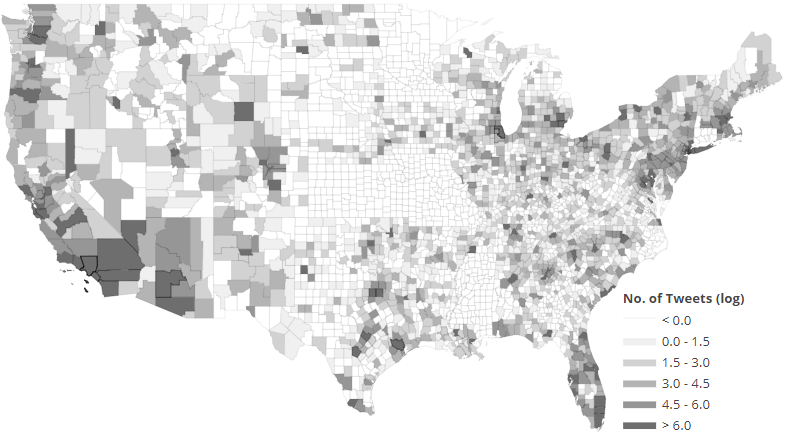
\includegraphics[width=.98\linewidth]{figures/map-tweets.png}
	\caption{\textsc{Geographical Distribution of MeToo Tweets in 2018}}
	\label{fig:choropleth-tweets}
\end{figure}

\clearpage
\FloatBarrier
%-------------------------------------------------------------------------------
\section{MeToo Tweet Content}
\label{sm:text}
%-------------------------------------------------------------------------------
This appendix reports analyses of the MeToo geocoded tweet metadata and text content (\cref{sm:data}, n = 324k tweets).
The analyses implement complementary approaches to assess tweet authenticity and thematic content.
These analyses include a metadata analysis of the hashtag usage patterns and engagement metrics, extraction and analysis of URLs shared in the tweets, mentions (@) and hashtags, Named Entity Recognition (NER) to identify discussed figures and organizations, network analysis of mention patterns, and topic modeling to recover dominant themes.
Consistent across these various measures and methods, the tweets center on documented high-profile MeToo events and figures from 2018, particularly the Kavanaugh confirmation hearings, as well as movement founders and entertainment industry cases tied to the movement's origins (\crefrange{sec:mt-background}{sec:mt-timeline}).
MeToo tweets are highly politicized, with politically charged topics among the most engaging.
Major news outlets dominate both URL sharing and entity mentions, suggesting that much of the conversation occurred around mainstream media coverage of related real-world events.
Collectively, these analyses suggest the \#MeToo tweets are strongly tied to the MeToo discourse.

%===============================================================================
\subsection{Preprocessing}
I preprocess the tweet text before text analysis to remove Twitter artifacts, URLs, and duplicate text while maintaining semantic context.
First, URLs are removed as they do not contribute semantic content.
I remove them using the \texttt{URLExtract} Python package (\url{https://github.com/lipoja/URLExtract}), which locates URLs in tweet text by identifying Top-Level Domains (TLDs) from the IANA registry and then expanding boundaries in both directions until reaching stop characters (whitespace, commas, quotes).
I remove repeated punctuation marks (e.g., This is terrible!!!'' becomes This is terrible!'') and excessive white spaces.
I also remove consecutive repeated words and phrases.
For example, ``metoo metoo metoo'' becomes ``metoo'', i support ``metoo \#metoo movement'' becomes ``i support metoo movement'', and ``\#timesup \#metoo timesup metoo'' becomes ``\#timesup \#metoo''.
This deduplication treats words with and without hashtag or mention symbols as identical for comparison purposes (so metoo'' and \#metoo'' are considered duplicates, as are @Trump'' and ``Trump''), while preserving whichever variant appears first.
This deduplication checks for repeated single words, word pairs, and three-word phrases.
I preserve @mentions and \# symbols as these contain substantive information about tweet targets and movement-related discourse.

%===============================================================================
\subsection{Tweet metadata}

First, I examine the distribution of \#metoo tweets in 2018 per author (via the \textit{account ID}).
Contrary to bot-like spamming behavior to generate fake support or activity, the median user posted only 1 tweet (mean = 2.66), with 95\% of users posting 7 or fewer tweets in 2018.
Fewer than 0.1\% of accounts posted more than a 100 \#metoo tweets.
This distribution is inconsistent with automated spam or coordinated organizational campaigns, to the extent that they involve high-volume posting from a small set of accounts.

Most tweets have only a few hashtags (\cref{fig:hashtag_density_ecdf}): 55\% have just one (the \#metoo), 73.5\% have two (see \cref{fig:network_hashtags} for top co-occurring hashtags).
Spam or bot behavior might involve excessive hashtag stuffing, but only 10\% of the sample have more than five hashtags.
The long tail may include politically engaged users who employ multiple movement-related tags (e.g., \#MeToo, \#TimesUp) (\cref{fig:top_hashtags_tabulation}).
\cref{fig:retweets_fave_scatter} shows the bivariate distribution of favorites and retweets.
Many tweets have low or zero engagement, but favorites and retweets are strongly correlated ($\hat{p} = .92$).

\begin{figure}
	\centering
	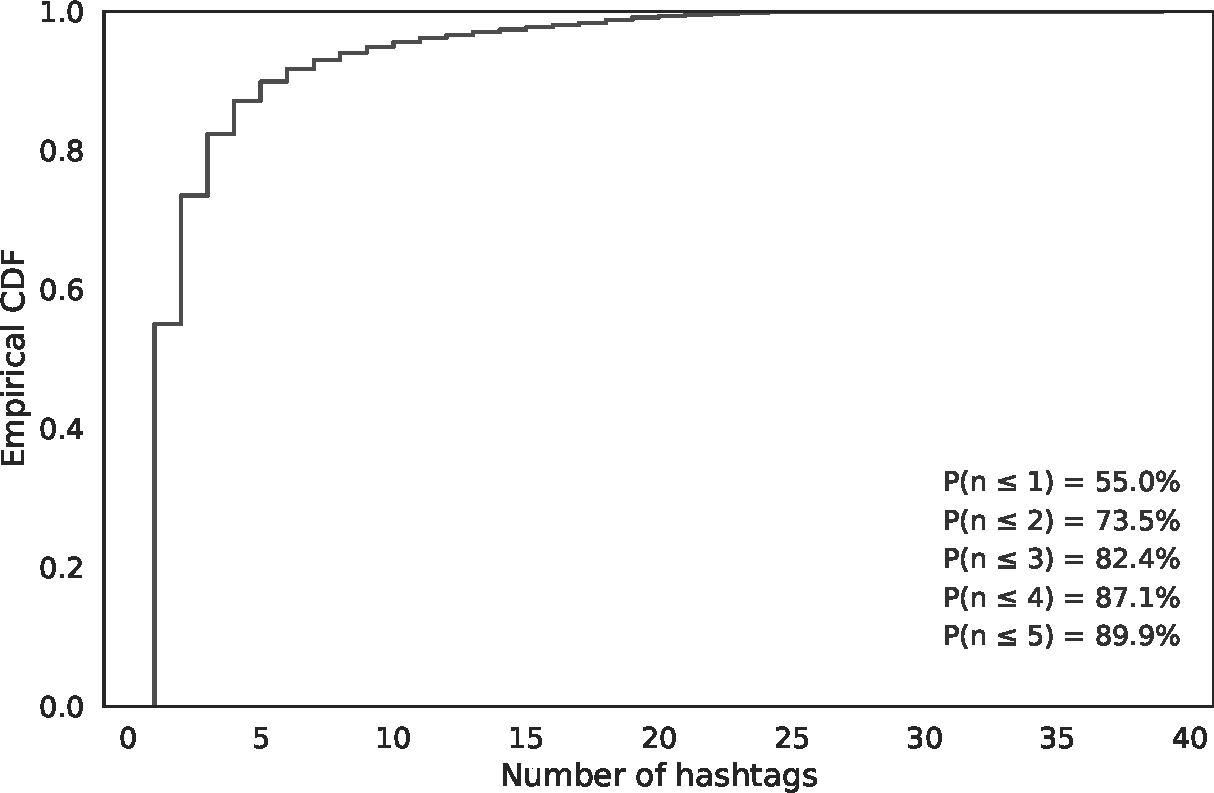
\includegraphics[width=.6\linewidth]{figures/hashtag_density_ecdf.pdf}
	\caption{
		Cumulative Distribution Function of the Number of Hashtags per MeToo Tweet.
	}
	\label{fig:hashtag_density_ecdf}
\end{figure}

\begin{figure}
	\centering
	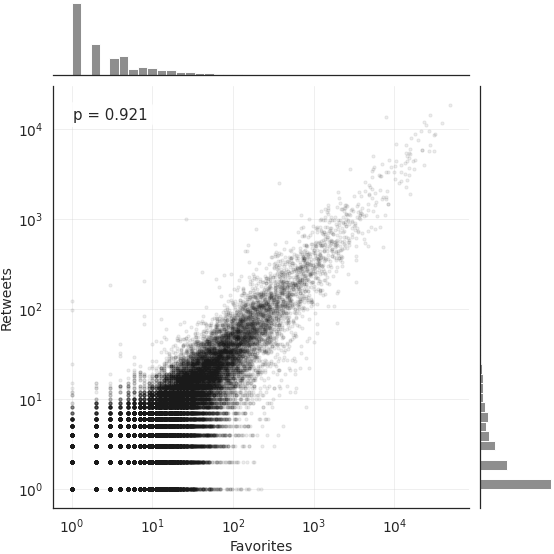
\includegraphics[width=.6\linewidth]{figures/retweets_fave_scatter.png}
	\caption{
		Bivariate Distribution of Tweet Favorites and Retweets.
		Notes: Scatterplot of geocoded tweets from 2018.
		Both axes x are on a log scale.
		Pearson correlation coefficient ($p$) shown in upper left.
	}
	\label{fig:retweets_fave_scatter}
\end{figure} 

\begin{figure}
	\centering
	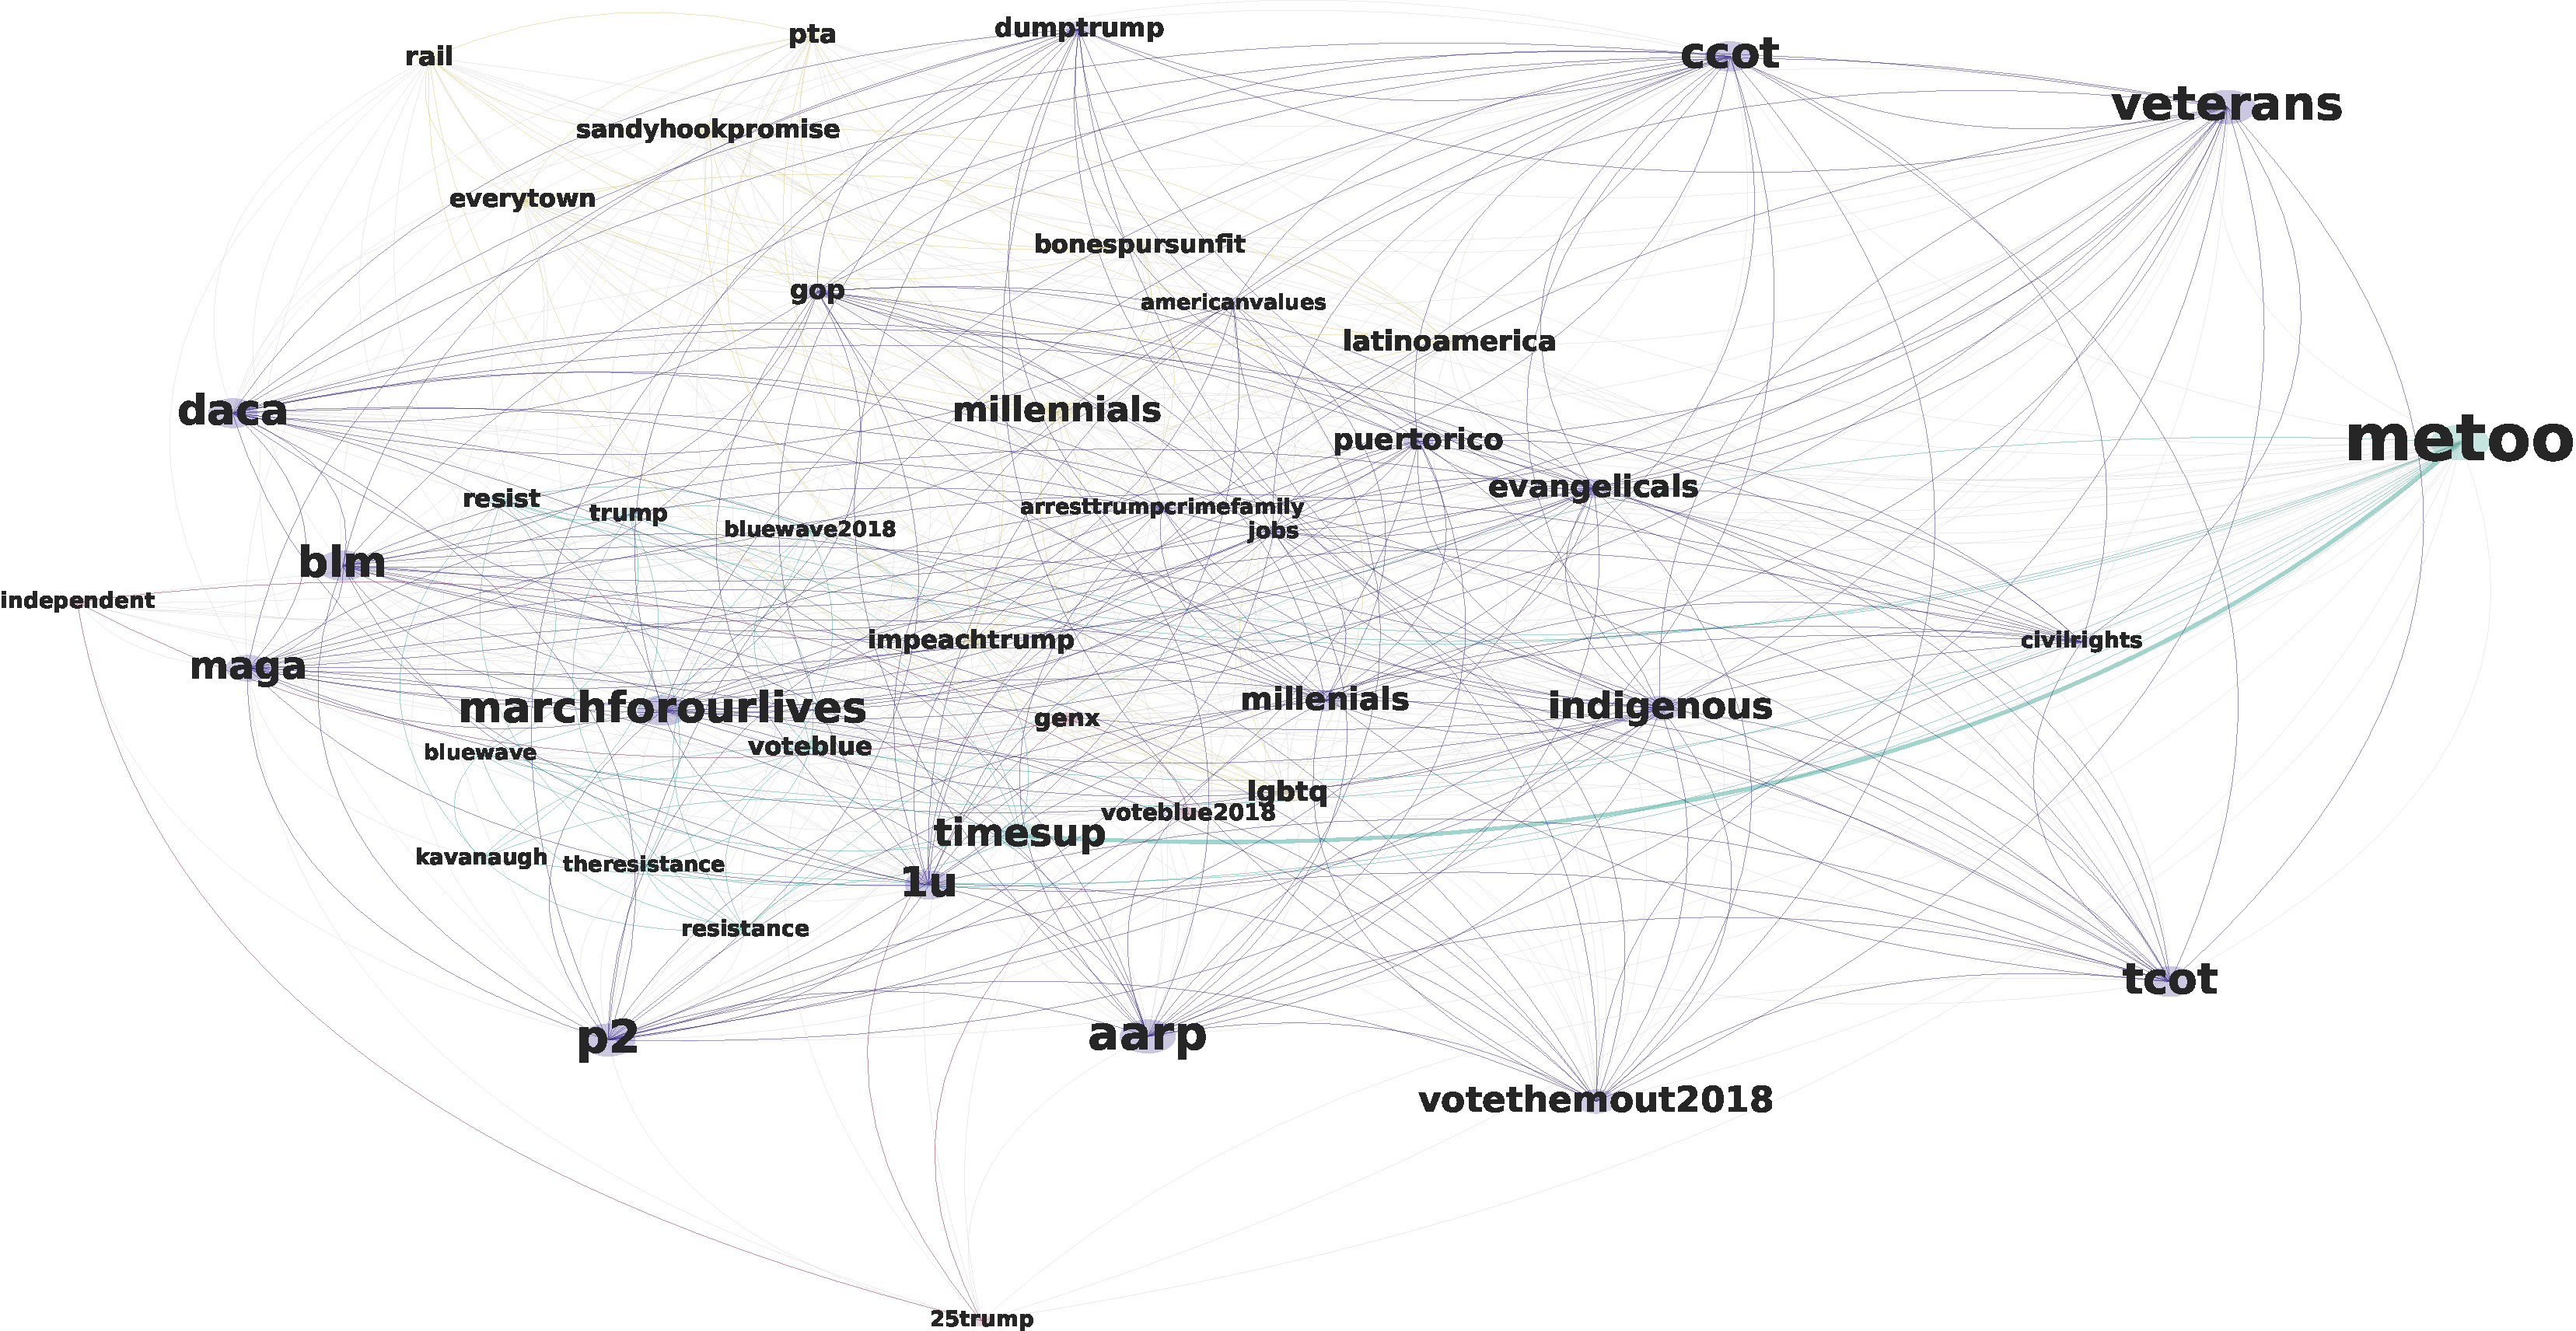
\includegraphics[width=\linewidth]{figures/network_hashtags.pdf}
	\caption{
		Network of top co-occurring hashtags.\\
		Notes: Network includes hashtag pairs with $\geq$1,000 co-occurrences, filtered to the top nodes (by weighted degree, with a minimum of 10 connections).
		Hashtags include electoral mobilization tags (timesup, voteblue2018, bluewave2018, p2 [Progressives 2.0], marchforourlives), demographic tags (millennials, genx, veterans, aarp [American Association of Retired Persons]), gun safety movements (sandyhookpromise, everytown), immigration and social justice (daca[Deferred Action for Childhood Arrivals], indigenous, blm, latinoamerica, puertorico), and anti-Trump organizing (resist, impeachtrump, arresttrumpcrimefamily, bonespursunfit).
	}
	\label{fig:network_hashtags}
\end{figure}

\begin{figure}
	\centering
	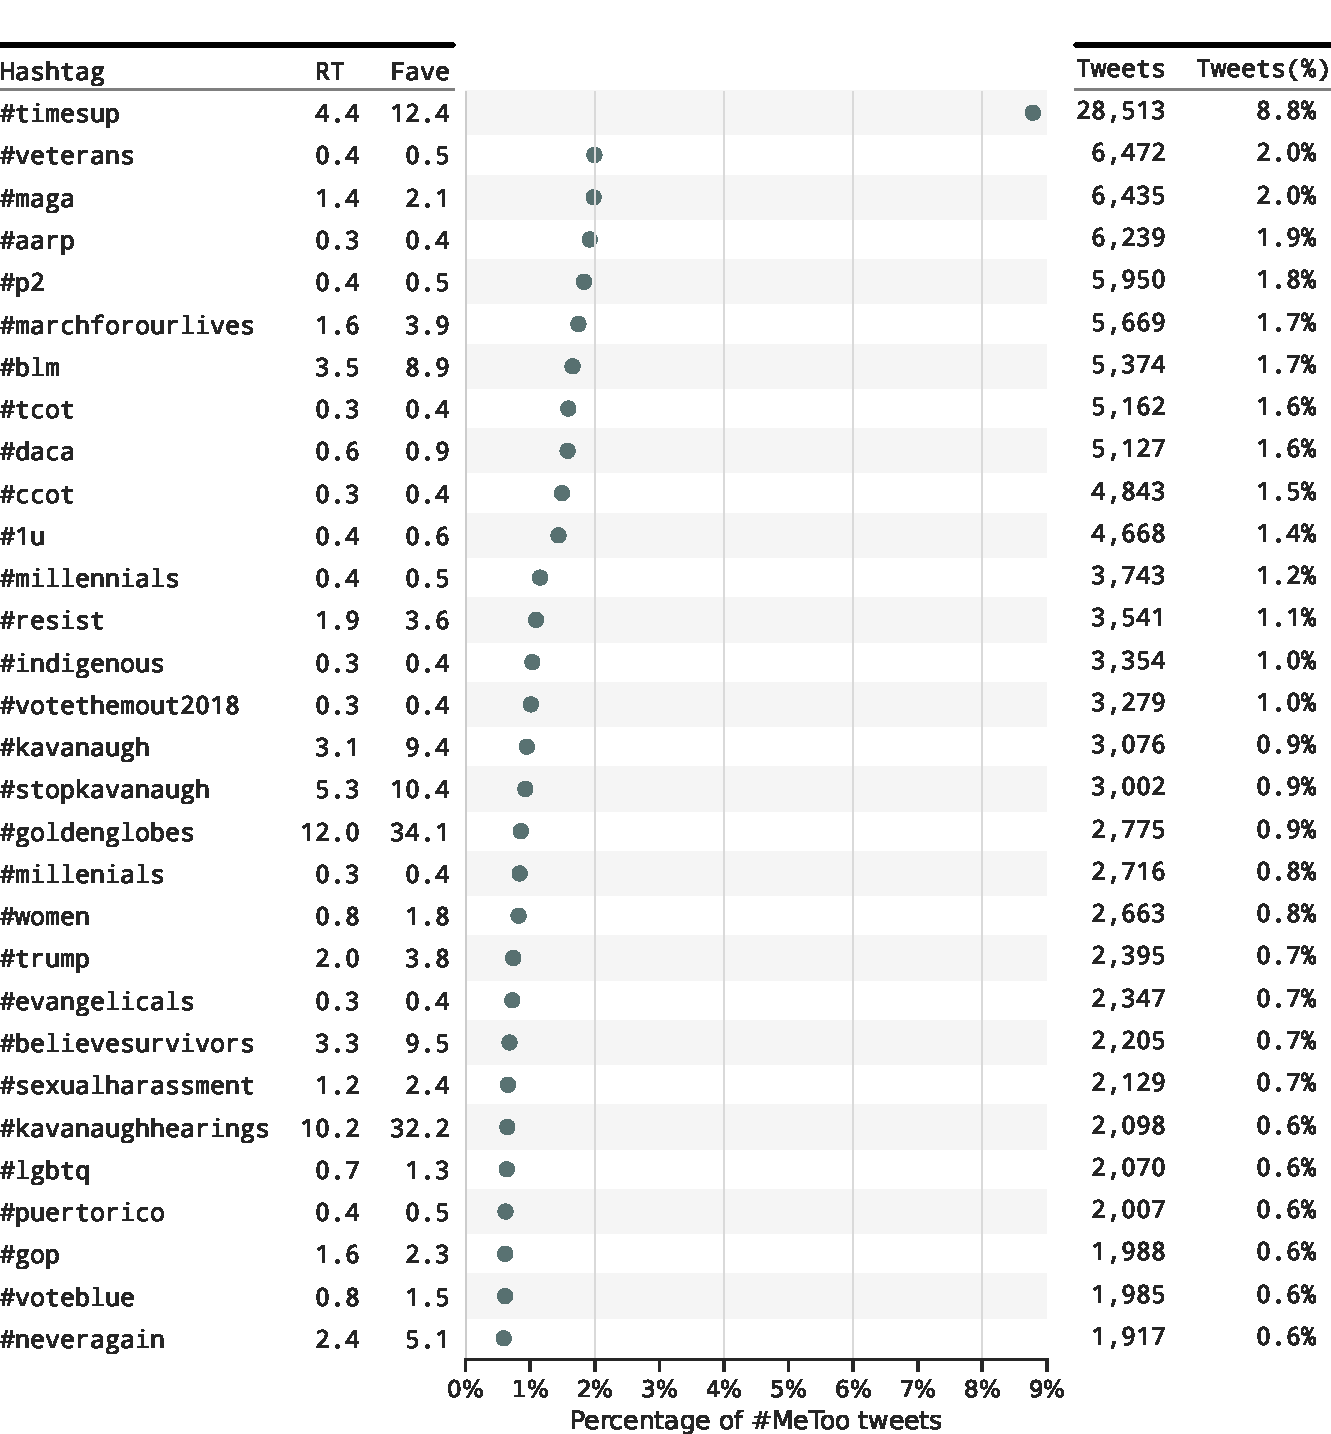
\includegraphics[width=\linewidth]{figures/top_hashtags_tabulation.pdf}
	\caption{
		30 most frequent co-occurring hashtags with \#MeToo.\\
		Notes: RT = mean retweets per tweet containing the hashtag.
		Fave = mean favorites per tweet containing the hashtag.
	}
	\label{fig:top_hashtags_tabulation}
\end{figure} 

\begin{figure}
	\centering
	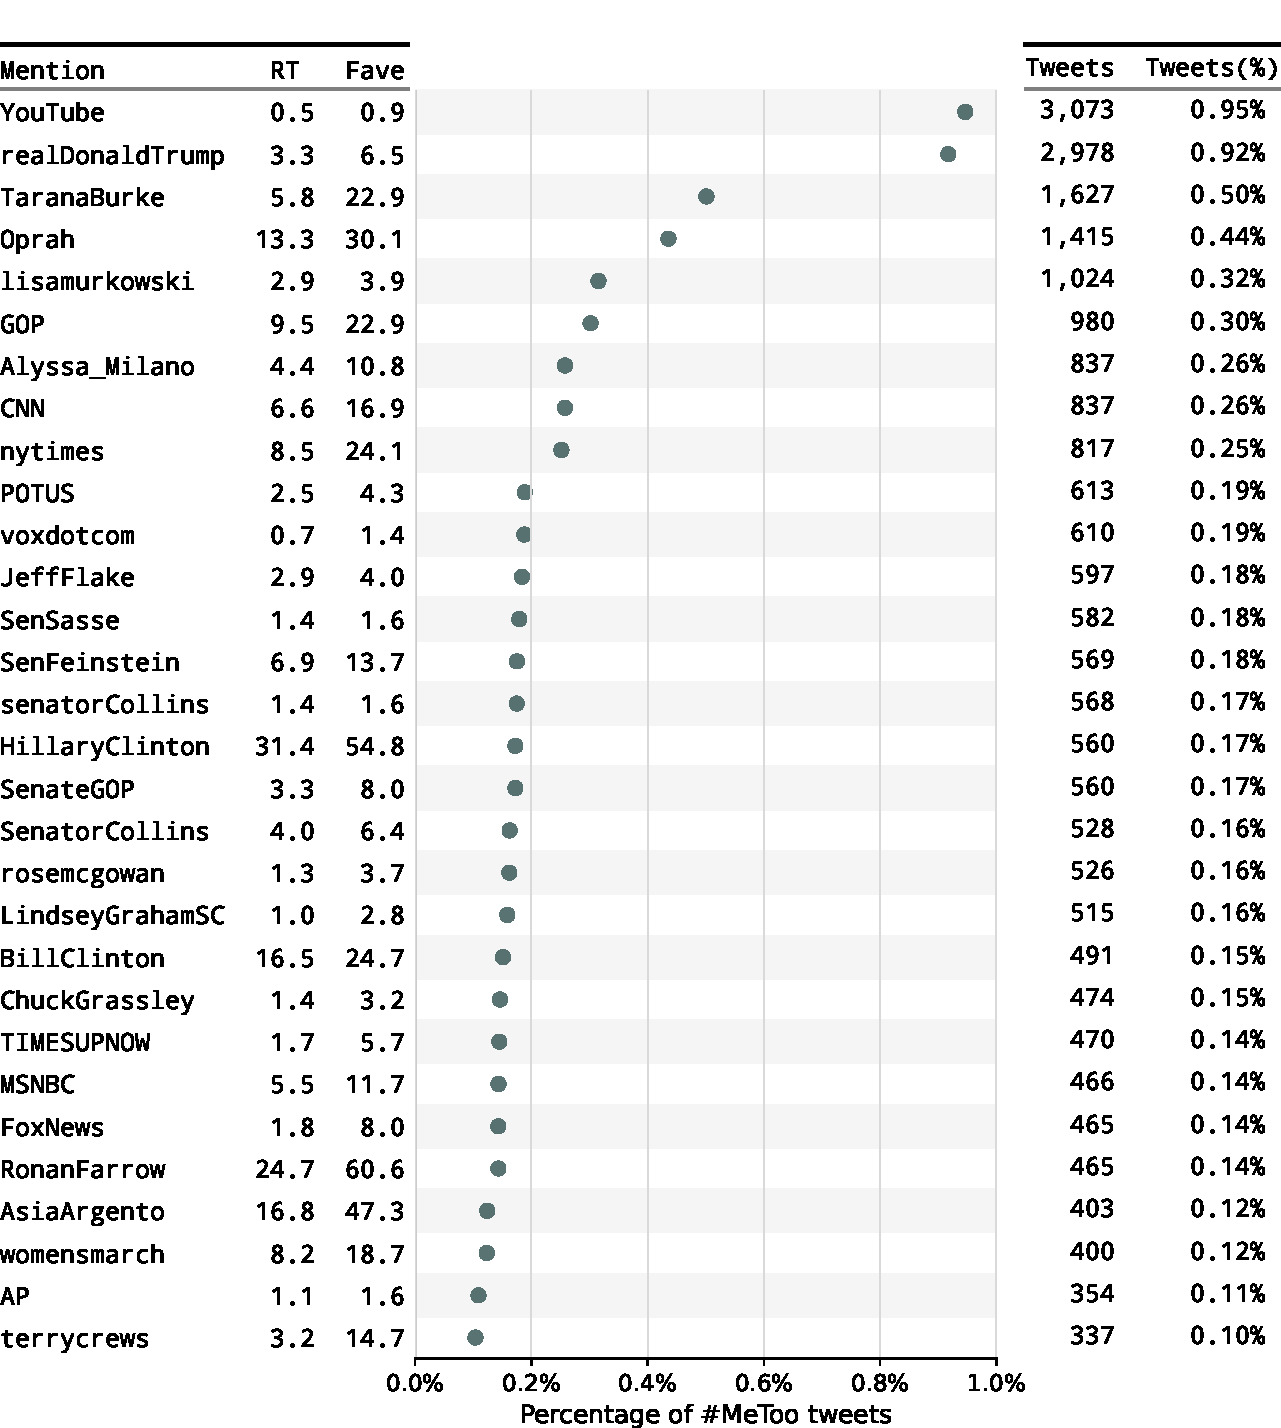
\includegraphics[width=\linewidth]{figures/top_mentions_tabulation.pdf}
	\caption{
		30 most frequent mentions (``@'') with \#MeToo.\\
		Notes: RT = mean retweets per tweet containing the hashtag.
		Fave = mean favorites per tweet containing the hashtag.
		n = 324k geocoded tweets from 2018.
	}
	\label{fig:top_mentions_tabulation}
\end{figure} 

\begin{figure}
	\centering
	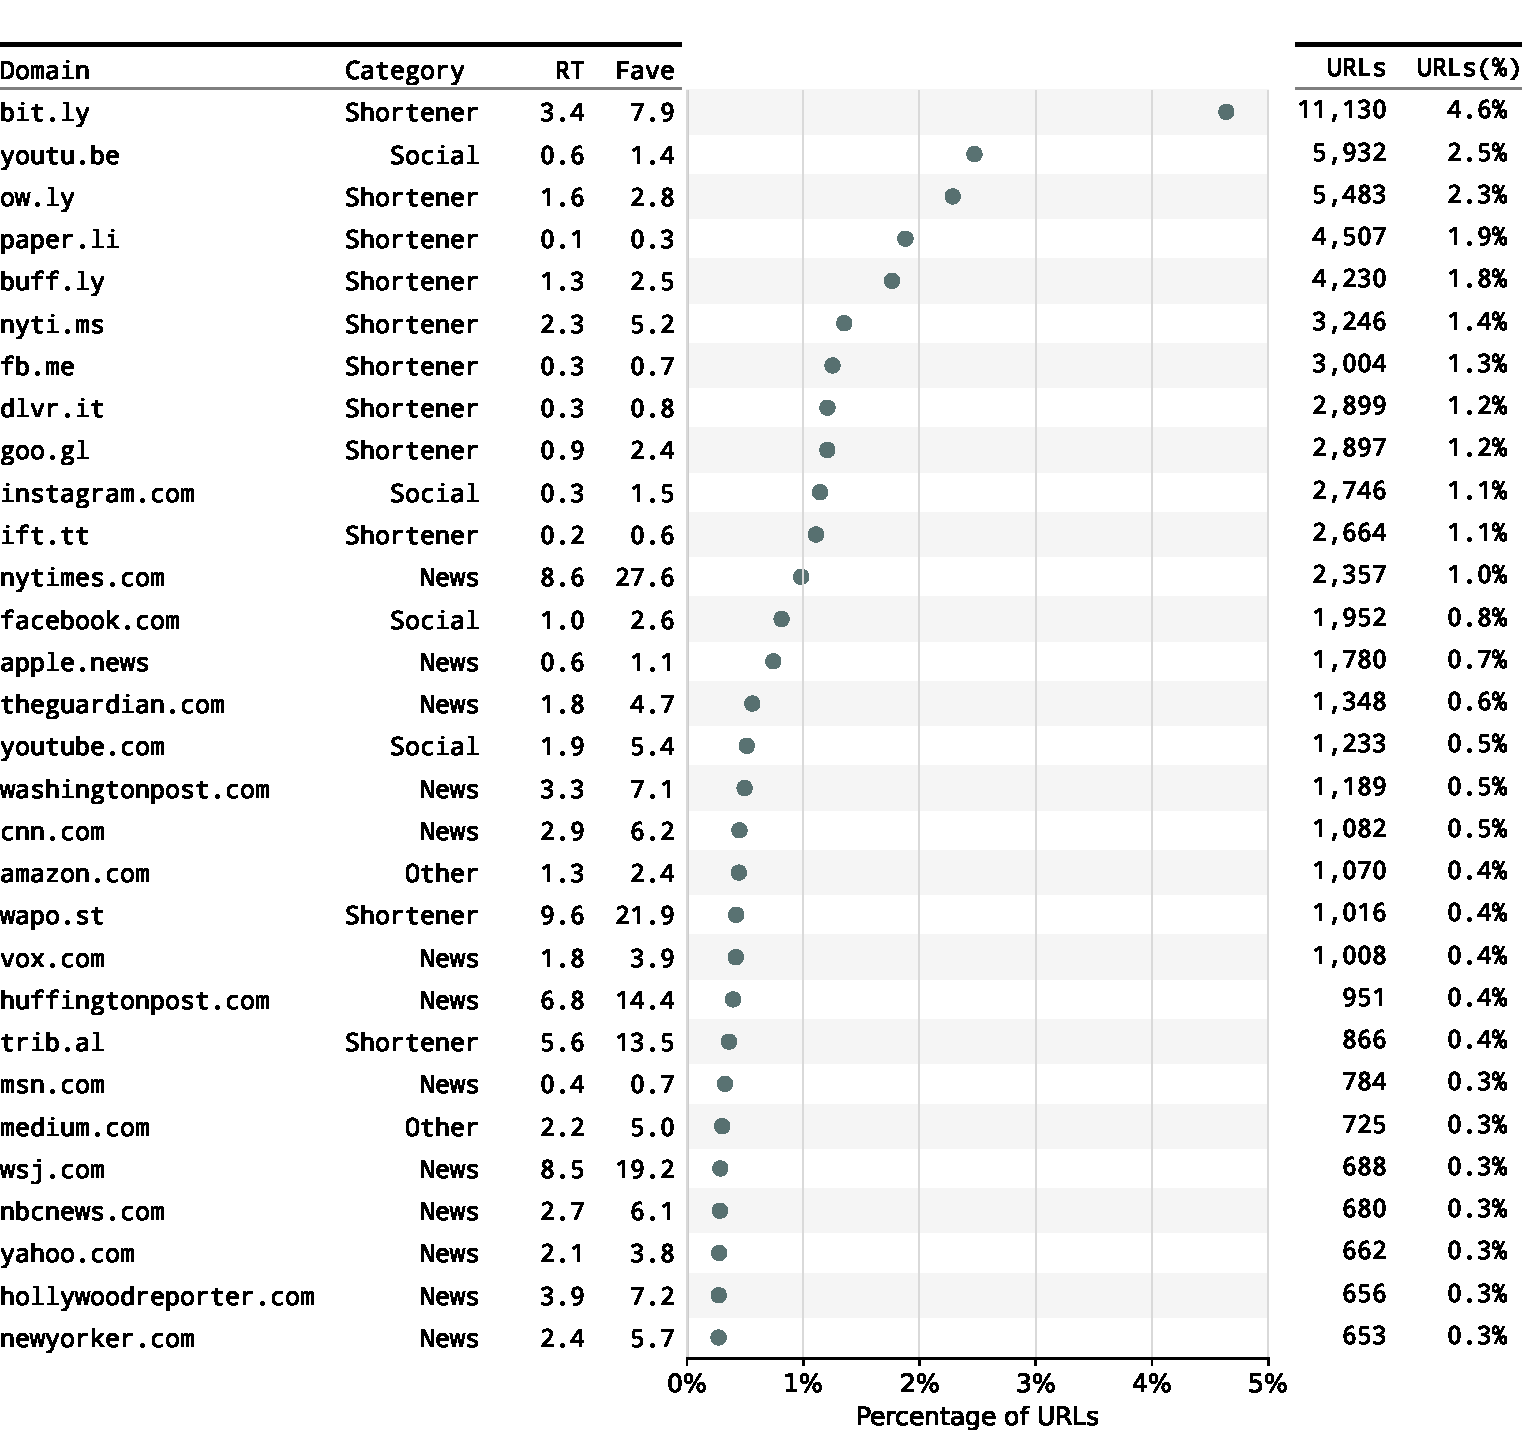
\includegraphics[width=\linewidth]{figures/top_domains_tabulation.pdf}
	\caption{
		30 most frequent domains with \#MeToo.\\
		Notes: RT = mean retweets per tweet containing the hashtag.
		Fave = mean favorites per tweet containing the hashtag.
		URLs are extracted using the \texttt{urlextract} package, and domains of URLs are extracted using the \texttt{tldextract} package.
	}
	\label{fig:top_domains_tabulation}
\end{figure} 

\begin{table}
	\centering
	\caption{Top Named Entities Extracted from Geocoded Human Tweets}
	\label{tab:ner_results}
	\small
	\begin{adjustbox}{max width=\textwidth}
		\begin{tabular}{@{}lr|lr|lr|lr@{}}
			\toprule
			\multicolumn{2}{c}{\textbf{PERSON}} & \multicolumn{2}{c}{\textbf{ORG}} & \multicolumn{2}{c}{\textbf{GPE}} & \multicolumn{2}{c}{\textbf{NORP}} \\
			\midrule
			Oprah & (2,974) & Trump & (5,046) & Hollywood & (4,145) & Democrats & (1,721) \\
			Kavanaugh & (2,029) & GOP & (3,619) & America & (1,846) & American & (1,121) \\
			Bill Clinton & (1,867) & CNN & (1,378) & US & (1,091) & Republicans & (1,087) \\
			Harvey Weinstein & (1,540) & TaranaBurke & (1,367) & China & (863) & Democrat & (841) \\
			Ford & (1,537) & FBI & (1,365) & California & (719) & Dems & (769) \\
			Bill Cosby & (1,455) & YouTube & (1,230) & Montana & (644) & Republican & (744) \\
			Weinstein & (1,307) & CBS & (1,031) & U.S. & (487) & Russian & (628) \\
			Monica Lewinsky & (1,104) & Kavanaugh & (979) & New York & (430) & Americans & (591) \\
			Tarana Burke & (1,048) & Congress & (925) & Russia & (370) & French & (562) \\
			Aziz Ansari & (1,014) & Time & (907) & India & (318) & Democratic & (369) \\
			Christine Blasey Ford & (1,004) & MAGA & (843) & Washington & (299) & Southern Baptists & (317) \\
			Anita Hill & (926) & Twitter & (830) & NY & (298) & Chinese & (299) \\
			Cosby & (884) & Senate & (818) & Texas & (284) & democrats & (249) \\
			Clinton & (855) & NYT & (802) & USA & (280) & Christian & (226) \\
			Brett Kavanaugh & (846) & SCOTUS & (722) & DC & (267) & Jewish & (206) \\
			Trump & (790) & MeToo Movement & (651) & Chicago & (267) & Muslim & (204) \\
			Catherine Deneuve & (729) & MSNBC & (623) & France & (240) & Dem & (197) \\
			lisamurkowski & (655) & SenSasse & (578) & Massachusetts & (233) & Catholic & (176) \\
			Bill & (621) & Supreme Court & (539) & U.S & (224) & British & (170) \\
			Hillary & (606) & FoxNews & (520) & United States & (207) & democrat & (145) \\
			Donald Trump & (604) & NYTimes & (519) & LA & (201) & dems & (132) \\
			Woody Allen & (594) & nytimes & (518) & Florida & (188) & republicans & (129) \\
			Ruth Bader Ginsburg & (567) & BillClinton & (489) & Japan & (185) & Indian & (114) \\
			Sean Penn & (555) & AP & (488) & Colorado & (172) & WSJOpinion & (112) \\
			Stormy Daniel & (526) & AsiaArgento & (459) & Dallas & (166) & Christians & (109) \\
			Charlie Rose & (470) & Ford & (456) & UK & (157) & republican & (98) \\
			Eric Schneiderman & (421) & Facebook & (450) & Israel & (147) & Canadian & (95) \\
			Obama & (405) & NBC & (418) & Canada & (145) & Pocahontas & (93) \\
			Ruth Bader & (403) & RonanFarrow & (408) & South Korea & (145) & LGBTQ & (89) \\
			R. Kelly & (402) & NPR & (403) & South Africa & (135) & MiraSorvino & (88) \\
			\bottomrule
		\end{tabular}
	\end{adjustbox}
	\caption*{
		\footnotesize
		\textit{Notes:} Named entities extracted using \texttt{spaCy}'s \texttt{en\_core\_web\_lg} model. PERSON: people, including fictional characters; ORG: companies, agencies, institutions; GPE: geo-political entities (countries, cities, states); NORP: nationalities or religious/political groups. Numbers in parentheses indicate frequency of mentions.
	}
\end{table}

\cref{fig:top_hashtags_tabulation} lists the 30 most frequently co-occurring hashtags with \#metoo \citep{forestplot}.
Electoral mobilization tags appear prominently: \#timesup (8.8\%), \#marchforourlives (1.7\%), \#p2 (1.8\%), and \#votethemout2018 (1.0\%).
Kavanaugh hearing-related hashtags cluster together: \#kavanaugh (0.9\%), \#stopkavanaugh (0.9\%), \#kavanaughhearings (0.6\%), and \#believesurvivors (0.7\%).
Other hashtags relate to immigration issues (\#daca, 1.6\%), racial justice (\#blm, 1.7\%), and gun control policies (\#everytown).
Engagement varies across hashtags: the top co-occuring \#timesup averages 4.4 retweets and 12.4 favorites, \#kavanaughhearings averages 10.2 retweets and 32.2 favorites, while generic tags like \#p2 have 0.4 retweets and 0.5 favorites.
(See also the network of top co-occurring hashtags in \cref{fig:network_hashtags}.)
The high engagement relating to \#kavanaughhearings is consistent with the September-October 2018 spike in \#metoo tweets during the confirmation hearings.

\cref{fig:top_mentions_tabulation} lists the 30 most frequently mentioned accounts by usernames (identified by extracting the ``@''s).
The most mentioned figures relate to key proponents and those implicated in sexual harassment cases: Oprah (0.95\%, likely related to her Golden Globes speech), realDonaldTrump (0.92\%), TaranaBurke (0.50\%, founder of the \#MeToo movement), and lisamurkowski (0.32\%, Alaskan Republican Senator who ultimately voted against Kavanaugh's confirmation).
Political figures and entities appear prominently: GOP (0.30\%), POTUS (0.19\%), senators including SenSasse (0.18\%), senatorCollins (0.17\%), SenatorCollins (0.16\%), JeffFlake (0.18\%), SenFeinstein (0.18\%), and LindseGrahamSC (0.16\%), as well as HillaryClinton (0.17\%) and BillClinton (0.15\%).
Mentions of media organizations and journalists are common: CNN (0.26\%), The New York Times (0.25\%), MSNBC (0.14\%), Fox News (0.14\%), Vox.com (0.19\%), AP (0.11\%), and RonanFarrow (0.14\%), consistent with news outlets dominating the top domains (\cref{fig:top_domains_tabulation}).
The prominence of political figures (particularly Collins [@senatorCollins, @SenatorCollins], Flake [@JeffFlake], Murkowski [@lisamurkowski], Feinstein [@SenFeinstein], and Graham [@LindseGrahamSC]) reflects the Kavanaugh confirmation debate (\crefrange{sec:mt-background}{sec:mt-timeline}).

\cref{fig:top_domains_tabulation} lists the 30 most frequently linked domains across 310,184 tweets containing URLs (95.5\% of the corpus).
URLs are extracted using \texttt{urlextract}.
Domains are then parsed using the \texttt{tldextract} package (\url{https://github.com/john-kurkowski/tldextract}), which accurately separates URLs into subdomain, domain, and public suffix components using the Public Suffix List (\url{https://publicsuffix.org/}).
This approach handles edge cases that naive splitting on dots would fail to parse correctly (e.g., forums.bbc.co.uk) and works for both full URLs (e.g., https://www.nytimes.com/article) and URL shorteners (e.g., bit.ly links).
Major news outlets appear frequently: nytimes.com (1.0\% of URL tweets, 8.6 mean retweets, 27.6 mean favorites), theguardian.com, washingtonpost.com, cnn.com, vox.com, huffingtonpost.com, and wsj.com.
URL shorteners are also prevalent (bit.ly [4.6\%], youtu.be [2.5\%], ow.ly [2.3\%], and buff.ly [1.8\%]), as are social media platforms (instagram.com, facebook.com, and youtube.com).
Tweets with wapo.st URLs have the highest engagement (9.6 mean retweets and 21.9 favorites).
See also \cref{fig:network_mentions} showing the major news outlets frequently cited within the tweet network.

\cref{fig:network_mentions} shows the 30 most-mentioned Twitter accounts within a network of accounts mentioning (``@'') each other.
Consistent with \cref{fig:top_mentions_tabulation} and \cref{fig:top_domains_tabulation}, most mentioned people in the network include key people related to the founding of the movement (e.g., Tarana Burke, \cref{sec:mt-background}), people as central figures in the ``referendum'' (e.g., Trump, POTUS), political figures (e.g., senators Collins, Flake, Murkowski, Sasse) related to the Kavanaugh hearings, and media organizations and journalists (e.g., Ronan Farrow, NYT, MSNBC, Fox News), and related movements (e.g., womensmarch, timesupnow).

%===============================================================================
\subsection{Named entities}
To identify named entities in the MeToo tweets, I use \texttt{spaCy}'s \texttt{en\_core\_web\_lg model}, a model trained on web-written text (blogs, news, comments).
\cref{tab:ner_results} reports the 30 most frequently mentioned entities across four categories: persons (PERSON), organizations (ORG), geopolitical entities (GPE), and nationalities or religious/political groups (NORP).
The model incorrectly names ``MeToo'' as a PERSON, which I exclude from \cref{tab:ner_results}.

The PERSON entities largely mirror the most frequently mentioned accounts (\cref{fig:top_mentions_tabulation}) and reflect central figures in both harassment allegations and political responses.
Frequently mentioned individuals include Oprah Winfrey (likely tied to her Golden Globes speech), Brett Kavanaugh and Christine Blasey Ford (Kavanaugh confirmation hearings), Tarana Burke (movement founder), and high-profile figures implicated in cases of sexual assault, such as Harvey Weinstein and Bill Cosby.
Historical cases, notably Bill Clinton and Monica Lewinsky (not captured in top mentions), also feature prominently, consistent with retrospective reassessments triggered by the movement.

ORG entities are dominated by media outlets and political institutions, including major news organizations (e.g., CNN, Fox News, NYT, AP), social media platforms, and government and legislative bodies (e.g., the Senate, Congress, and the Supreme Court).
This pattern aligns closely with the domain-level URL analysis (\cref{fig:top_domains_tabulation}), reinforcing that the \#MeToo discourse on Twitter was heavily mediated by journalistic coverage.

GPE entities have a strong US-centric concentration, with frequent references to Hollywood, the United States, California, and Washington, D.C.
Hollywood is also prominent, reflecting the movement's early origins in the entertainment industry (\cref{sec:mt-timeline}), while Washington-related mentions cluster around elite political conflict, likely related to the Kavanaugh hearings.

Finally, the NORP category highlights the partisan and identity-based framing of \#MeToo discourse, suggesting that the \#MeToo engagement on Twitter was characterized by substantive political contestation and mobilization rather than discussion confined solely to individual allegations of sexual harassment.

%===============================================================================
\subsection{Topics}
To recover the dominant themes in \#MeToo tweets---where a ``topic'' is a set of terms that tend to co-occur across semantically similar tweets---I use BERTopic instead of classical bag-of-words topic modeling approaches since we want semantically-aware groups of tweets \citep{bertopic, neutrality}. 
Specifically, I use a transformer-based topic modeling pipeline that combines sentence embeddings with density-based clustering to identify topics in the \# metoo tweets \citep{bertopic}.
Tweets are embedded using the \texttt{all-mpnet-base-v2} sentence-transformer model and then projected to a lower-dimensional space using UMAP (neighbors = 30, components = 5).
To reduce noise from short tweets, I remove tweets that have fewer than two tokens after preprocessing and deduplicating words, for a total of 305{,}133 tweets.
Topics are formed by clustering the reduced embeddings with HDBSCAN (min. cluster size = 300).
For topic representations, I use a bag-of-words vocabulary constructed with a \texttt{CountVectorizer} over unigrams, with English stopwords removed, and I summarize each topic using the highest-weight terms.

\begin{figure}
	\centering
	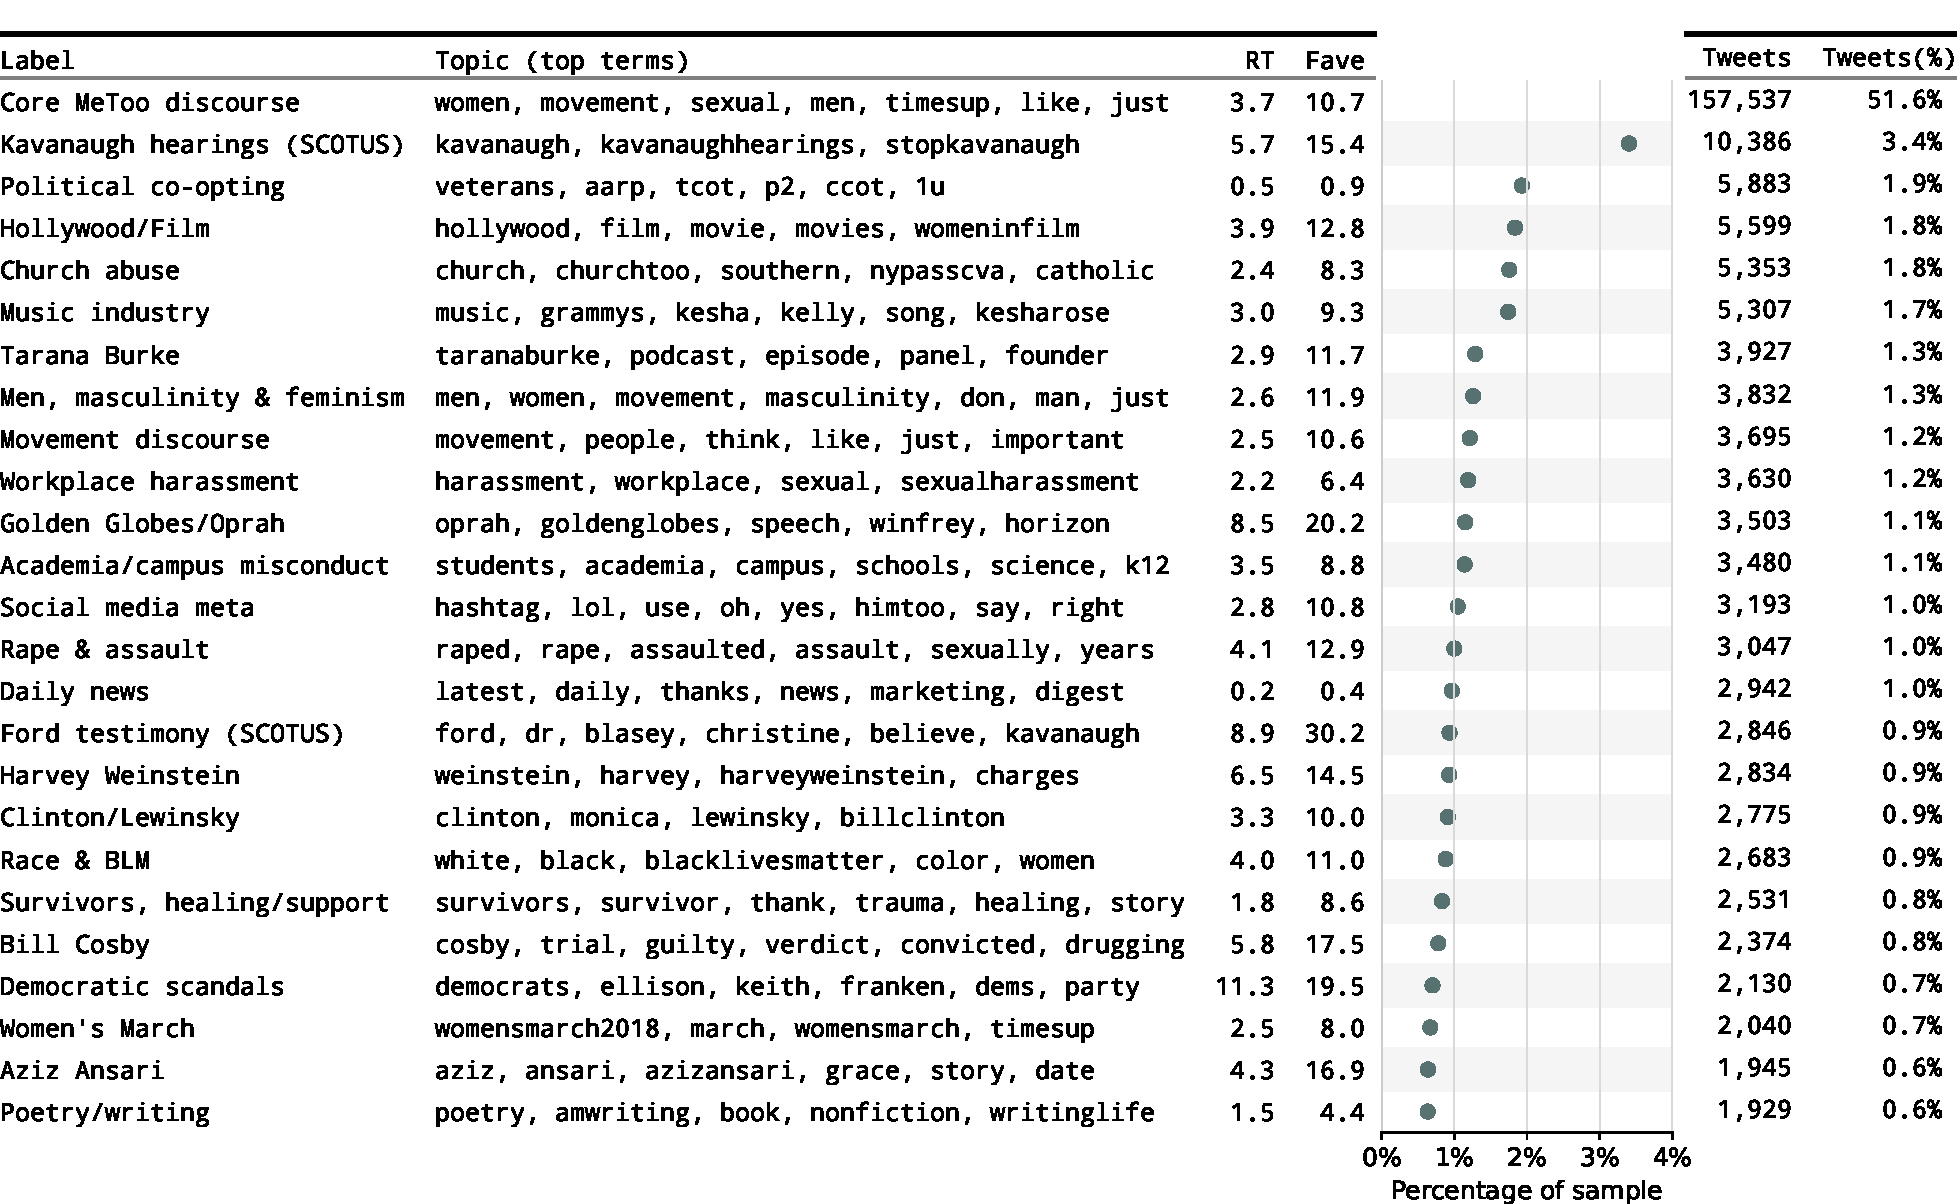
\includegraphics[width=\linewidth]{figures/top_topics_tabulation.pdf}
	\caption{
		25 most frequent topics with \#MeToo.\\
		Notes: RT = mean retweets per tweet containing the hashtag.
		Fave = mean favorites per tweet containing the hashtag.
		The core topic (first row) marker is not plotted as it is out of range.
		Second column shows the most common terms within the topic clusters.
		These 25 topics collectively account for over 87\% of the tweet sample.
		See \cref{fig:topic_2Dmap} for a 2D projection of these topics.
	}
	\label{fig:top_topics_tabulation}
\end{figure}

\cref{fig:topic_2Dmap} visualizes the topic structure by embedding tweets into a two-dimensional space using UMAP, which preserves semantic relationships between tweets.
The core MeToo discourse topic, which comprises 51.6\% of the sample, forms a dense central cluster (labeled the ``outlier'' topic in BERTopic), with keywords including women, movement, sexual, men, and timesup.
The spatial separation between clusters suggests thematic coherence within topics and distinction across topics.
The proximity of related topics indicates semantic similarity, for example, tweets on Christine Blasey Ford clustered near Brett Kavanaugh, Rape near Survivors healing/support, Workplace harassment near Academic/campus misconduct, and Harvey Weinstein near Hollywood/Film.

\cref{fig:top_topics_tabulation} enumerates these topics, their sample distribution, Twitter engagement (favorites and retweets), and top terms identified using class-based term frequency–inverse document frequency (c-TF-IDF).
Topics with the highest engagement tend to be politically charged (e.g., the Kavanaugh hearings averaged 5.7 retweets and 15.4 favorites, and the Ford testimony averaged 8.9 retweets and 30.2 favorites).

\FloatBarrier
%-------------------------------------------------------------------------------
\section{MeToo Tweets Samples}
\label{sm:random-samples}
%-------------------------------------------------------------------------------
\begin{table}[htbp]
	\centering
	\scriptsize
	\setlength{\defaultaddspace}{6pt}
	\caption{Random Sample: State of the Union Day (n=20 from 1,006 on Jan 31, 2018)}
	\label{tab:sotu-sample}
	\begin{adjustbox}{max width=1\textwidth}	
		\begin{tabular}{@{\hspace{0\tabcolsep}}r>{\raggedright\arraybackslash}p{13cm}rr>{\raggedright\arraybackslash}p{2.8cm}@{\hspace{0\tabcolsep}}}
			\toprule
			& Content & Fave & RT & Other hashtags \\
			\midrule
			1 & Lots to watch for in tonight's \#SOTU address -- reactions from FLOTUS, the \#metoo movement, implications for midterms, and all the Dreamers coming as guests [URL] & 0 & 0 & \#sotu \\
			\addlinespace
			2 & Is 007 too toxic for the \#MeToo era? [Guardian URL] & 0 & 0 & --- \\
			\addlinespace
			3 & jealous statement, you look great, but think about the \#metoo movement of the past year by women that have been victims of sexual assault, harassment or inequality. Does this really say \#timesup? No babydoll. This says I never want women to move past men's misogyny because it & 0 & 0 & \#timesup \\
			\addlinespace
			4 & Seattleite Leah Griffin is accompanying Sen. @PattyMurray to bring \#MeToo to \#SOTU. [URL] & 1 & 0 & --- \\
			\addlinespace
			5 & Mentoring After \#MeToo [URL] & 0 & 0 & --- \\
			\addlinespace
			6 & My Classic professor just made a terrible comparison with the battle of Troy and the \#Metoo movement and I am very tempted to drop this class. & 0 & 0 & --- \\
			\addlinespace
			7 & Diane Keaton joined Alec Baldwin, defending Woody Allen in the face of the \#MeToo movement. [URL] & 0 & 0 & --- \\
			\addlinespace
			8 & \#FYI Jailbird Congressman Michael Grimm's \#METOO: I Was Bad-Touched By The FBI! [URL] & 0 & 0 & \#fyi \\
			\addlinespace
			9 & Jody Allard (@sendvodka) wrote after \#MeToo, ``my sons are part of the problem.'' She and @ProfSonoraJha join us on \#KUOWrecord to discuss the next step: teaching kids about consent. & 2 & 0 & \#kuowrecord \\
			\addlinespace
			10 & ``There are only two options: make progress or make excuses.'' - @TonyRobbins \#metoo \#TimesUp & 2 & 0 & \#timesup \\
			\addlinespace
			11 & 4 documented details of corruption/injustice in Cook Co Courts [URL] \#Resistance \#metoo \#p2 \#GenX \#millenials \#AARP \#BLM & 0 & 0 & \#resistance, \#p2, \#genx, \#millenials, \#aarp, \#blm \\
			\addlinespace
			12 & Getting From \#MeToo And \#TimesUp To Real Change: ``We have to take that solidarity moment and turn it into real action, and that's the slogging hard work of real movement building.'' - @GloriaFeldt [URL] & 10 & 4 & \#timesup \\
			\addlinespace
			13 & \#MeToo @POTUS K.R.W. \#Sincerely \#KatherineRobinsonWhite \#Epic \#Hollywood \#Screenplay \#Ghostwriter of @JimCameron \#Titanic (1997 Film) \& \#Avatar Franchise et al [...] & 0 & 0 & \#sincerely, \#katherinerobinsonwhite, \#epic, \#hollywood \\
			\addlinespace
			14 & PDDNI Gordon: Every woman I know can tell you a story about not being treated with dignity and respect. Why were people so surprised by the actions that led to the \#MeToo movement? \#pcevents & 2 & 2 & \#pcevents \\
			\addlinespace
			15 & Frankel and Germino committed to wearing black to Trump's State of the Union speech to send a message of solidarity to the \#MeToo movement, @CarloniBrittany reports. [Twitter URL] & 1 & 1 & --- \\
			\addlinespace
			16 & Wow! Great acting!! Trump is taking CONTROL of our Country! Only Hollywood and Illegals are THE RESISTANCE...oh and let's not forget \#metoo Keep working for Soros and Obama & 9 & 1 & --- \\
			\addlinespace
			17 & \#MeToo and \#TimesUp need to start directing their followers to begin interactive, positive change discussions. Here's a great thread by @DrDebraSoh that is seeking solutions and positive dialog. [Twitter URL] & 0 & 0 & \#timesup \\
			\addlinespace
			18 & Stand w/ \#truckers to stop \#ELD that is killing American citizens [...] \#eldorme \#MeToo \#MAGA \#farmers \#Livestock \#musicians [...] & 1 & 1 & \#truckers, \#eld, \#eldorme, \#maga, \#farmers \\
			\addlinespace
			19 & State of the Union guests include tax cut beneficiaries, \#MeToo advocates and more Dreamers than ever [URL] & 0 & 0 & --- \\
			\addlinespace
			20 & Grammys 2018: Artists Sound Off on Sexism, Equality, Power of White Rose - When the Grammys rolled into New York City Sunday night, it appeared the only \#MeToo moment would be Kesha's rousing, star-studded performance of ``Praying'' [...] [URL] & 0 & 0 & --- \\
			\bottomrule
		\end{tabular}
	\end{adjustbox}
\end{table}

\begin{table}[htbp]
	\centering
	\scriptsize
	\setlength{\defaultaddspace}{6pt}
	\caption{Random Sample: Women's March Day (n=20 from 2,883 on Jan 21, 2018)}
	\label{tab:womens-march-sample}
	\begin{adjustbox}{max width=1\textwidth}	
		\begin{tabular}{@{\hspace{0\tabcolsep}}r>{\raggedright\arraybackslash}p{13cm}rr>{\raggedright\arraybackslash}p{2.8cm}@{\hspace{0\tabcolsep}}}
			\toprule
			& Content & Fave & RT & Other hashtags \\
			\midrule
			1 & Bill Maher mansplains \#MeToo \#WomensMarch2018 \#TimesUp \#SaturdayMorning [HuffPost URL] & 0 & 0 & \#womensmarch2018, \#timesup, \#saturdaymorning \\
			\addlinespace
			2 & Tired of politicians f-n Americans! \#MeToo \#DrainTheSwamp \#ShumerShutdown \#ReleaseTheMemo \#MAGA & 0 & 2 & \#draintheswamp, \#shumershutdown, \#releasethememo, \#maga \\
			\addlinespace
			3 & ``When we say all, we mean ALL... `Me too' is not new!'' - Kristin Shrimplin with @WomenHelpingWom \#WomenMarch2018 \#TimesUp \#MeToo & 1 & 0 & \#womenmarch2018, \#timesup \\
			\addlinespace
			4 & Open up @WhiteHouse, we're outside! \#DumpTrump \#WomensMarchDC @womensmarch \#MyBodyMyChoice \#metoo \#NoMeansNo \#TimesUp & 1 & 0 & \#dumptrump, \#womensmarchdc, \#mybodymychoice, \#nomeansno \\
			\addlinespace
			5 & \#MeToo: What to Do When You Are Harassed [URL] \#metoo \#musicindustry \#harassment \#music & 0 & 0 & \#musicindustry, \#harassment, \#music \\
			\addlinespace
			6 & Had a blast @ \#WomensMarch2018 \#marchoncolorado \#hearmytruth \#metoo \#Resistance & 0 & 0 & \#womensmarch2018, \#marchoncolorado, \#hearmytruth, \#resistance \\
			\addlinespace
			7 & In The Midst Of \#MeToo, What Type Of Man Do You Want To Be? [URL] & 0 & 0 & --- \\
			\addlinespace
			8 & just fuck everything \#MeToo [naughty news network URL] & 2 & 1 & --- \\
			\addlinespace
			9 & YESVeto proof \#DACA \#CHIP NOW \#IgnoreTrump \#BLM \#Millennials \#AARP \#veterans \#tcot \#metoo \#Independent \#GenX \#p2 \#GenZ \#LGBTW [...] & 1 & 0 & \#daca, \#chip, \#ignoretrump, \#blm, \#millennials, \#aarp \\
			\addlinespace
			10 & We can't inspire if we are presented only as victims. \#ImwithMathilde \#MeToo and the Marketing of Female Narrative via @NYTimes [URL] & 0 & 0 & \#imwithmathilde \\
			\addlinespace
			11 & Wow im crying and have goosebumps \#MeToo \#timesup thank you for sharing your story! \#WomensMarch & 1 & 0 & \#timesup, \#womensmarch \\
			\addlinespace
			12 & TIME'S UP BEASTS Laura Kipnis for @guardian; ``Women's bodies are still treated as public property by men. To miss that point is to miss the political importance and the political lineage of \#MeToo.'' & 0 & 0 & --- \\
			\addlinespace
			13 & So glad they have beautiful weather for the protests all over the country! \#TrumpShutdown \#metoo [NYT URL] & 0 & 0 & \#trumpshutdown \\
			\addlinespace
			14 & Women's rights are human rights \#Resist \#MeToo & 2 & 0 & \#resist \\
			\addlinespace
			15 & A view of the crowd with the March for Impeachment in downtown Portland. There's a \#MeToo march starting a few blocks away at 2pm @OPB & 38 & 14 & --- \\
			\addlinespace
			16 & The latest DCeiver People Things! [paper.li URL] Thanks to @imillhiser @recordedvoice @rebel19 \#trumpshutdown \#metoo & 4 & 2 & \#trumpshutdown \\
			\addlinespace
			17 & The Latest: New Jersey's first lady tells marchers, \#MeToo [URL] \#AccessNorthGA -ACCESS NORTH GA & 0 & 0 & \#accessnorthga \\
			\addlinespace
			18 & \#WomensMarch2018 \#timesup \#metoo & 0 & 0 & \#womensmarch2018, \#timesup \\
			\addlinespace
			19 & We march for a better, more just world. A world where no one has to say \#MeToo ever again. & 4 & 1 & --- \\
			\addlinespace
			20 & Back at it... \#WomenMarch2018 \#WomensMarchDC \#MeToo \#TimesUp & 1 & 2 & \#womenmarch2018, \#womensmarchdc \\
			\bottomrule
		\end{tabular}
	\end{adjustbox}
\end{table}

\begin{table}[htbp]
	\centering
	\scriptsize
	\setlength{\defaultaddspace}{6pt}
	\caption{Random Sample: Christine Blasey Ford Revelation Day (n=20 from 5,192 on Sep 17, 2018)}
	\label{tab:cbf-sample}
	\begin{adjustbox}{max width=1\textwidth}	
		\begin{tabular}{@{\hspace{0\tabcolsep}}r>{\raggedright\arraybackslash}p{13cm}rr>{\raggedright\arraybackslash}p{2.8cm}@{\hspace{0\tabcolsep}}}
			\toprule
			& Content & Fave & RT & Other hashtags \\
			\midrule
			1 & Bloomberg May Run for President as a Democrat. His Views on Policing and \#MeToo Could Be a Problem. [NYT URL] & 1 & 1 & --- \\
			\addlinespace
			2 & \#MeToo. & 1 & 0 & --- \\
			\addlinespace
			3 & Breaking \#ImWithHer \& \#MeToo News: sexist Texas politicians just voted to erase \#HillaryClinton \& \#HelenKeller from the State's textbooks [URL] & 0 & 1 & \#imwithher, \#hillaryclinton, \#helenkeller \\
			\addlinespace
			4 & Kavanaugh Classmate Named in \#MeToo Letter Breaks Silence [Western Journal URL] & 0 & 0 & --- \\
			\addlinespace
			5 & @SenatorCollins @lisamurkowski You let a man be the first in your party to think Ford should be heard? You are losing respect. Perhaps this no longer matters to you. \#MeToo & 0 & 0 & --- \\
			\addlinespace
			6 & Oh please!!!!!!! Give me a break. If it wasn't important 30 years ago, it's not important now. All the \#metoo generation, GO TO HELL. & 0 & 0 & --- \\
			\addlinespace
			7 & \#PostponeTheVote \#StopKavanaugh \#metoo \#WithdrawKavanaugh [Twitter URL] & 0 & 0 & \#postponethevote, \#stopkavanaugh \\
			\addlinespace
			8 & @JeffFlake I am heartened that you think the vote needs to be delayed. Attempted rape and assault is despicable and she has passed a lie detector test. He does not respect women and has lied under oath. Not suitable for SCOTUS. \#NoKavanaugh \#metoo [...] & 0 & 0 & \#nokavanaugh \\
			\addlinespace
			9 & Simple: Cavanaugh should withdraw until this matter is sorted out. He can always be reappointed when RBG's time is up. For now, Amy Coney Barrett can be confirmed right away. She has already completed a difficult confirmation...with no \#metoo accusations. Win/win & 0 & 0 & --- \\
			\addlinespace
			10 & Yall are all desperate and pathetic... Democrats are some of the lowest who only give a damn about themselves. Lol, accusation comes DECADES right before he's to get approved. Smells like bullshit to me just like \#MeToo [Twitter URL] & 1 & 0 & --- \\
			\addlinespace
			11 & \#MeToo & 2 & 0 & --- \\
			\addlinespace
			12 & Triggered triggered and triggered again \#ptsd \#metoo 5 wealthy frat boys, and me, the middle class freshman girl on her very first day at college, f-d up in the head for life \#KavaNO God bless this woman. Justice for her is some justice for me! & 427 & 58 & \#ptsd, \#kavano \\
			\addlinespace
			13 & Why \#MeToo still fails. [Apple News URL] & 0 & 0 & --- \\
			\addlinespace
			14 & Bloomberg May Run for President as a Democrat. His Views on Policing and \#MeToo Could Be a Problem. - The New York Times [Apple News URL] & 0 & 0 & --- \\
			\addlinespace
			15 & I believe Christine Blasey Ford. \#metoo & 1 & 0 & --- \\
			\addlinespace
			16 & \#metoo will support her. She's got thousands that have her back. & 1 & 0 & --- \\
			\addlinespace
			17 & \#MeToo & 3 & 0 & --- \\
			\addlinespace
			18 & ONLY @SenFeinstein had the information. Why hold it until July? No idea. BUT stop \& think about the political \& cultural climate right now. Trump, extreme partisanship, \#MeToo. It's a powder keg \& as we saw, it took EXACTLY 1 DAY for her name to be ``leaked''. \#StopKavanaugh & 0 & 0 & --- \\
			\addlinespace
			19 & .@SenatorCollins the entire country has its eye on you. This is when you make the decision on how you want to be remembered in the history books; as a coward who bent to the GOP or as a champion for all women. \#Kavanaugh \#MeToo \#PostponeTheVote [...] & 7 & 2 & \#kavanaugh, \#postponethevote \\
			\addlinespace
			20 & \#MeToo \#ChristineBlaseyFord \#KavaNOPE [Twitter URL] & 1 & 0 & \#christineblaseyford \\
			\bottomrule
		\end{tabular}
	\end{adjustbox}
\end{table}

\begin{table}[htbp]
	\centering
	\scriptsize
	\setlength{\defaultaddspace}{6pt}
	\caption{Random Sample: Christine Blasey Ford Testimony Day (n=20 from 7,362 on Sep 27, 2018)}
	\label{tab:testimony-sample}
	\begin{adjustbox}{max width=1\textwidth}	
		\begin{tabular}{@{\hspace{0\tabcolsep}}r>{\raggedright\arraybackslash}p{13cm}rr>{\raggedright\arraybackslash}p{2.8cm}@{\hspace{0\tabcolsep}}}
			\toprule
			& Content & Fave & RT & Other hashtags \\
			\midrule
			1 & Defending Kavanaugh, Trump laments \#MeToo as `very dangerous' for powerful men [WaPo URL] & 0 & 0 & --- \\
			\addlinespace
			2 & Given all that we know about sexual assault, and given the recent \#metoo revelations, and given the fact that single physician molested dozens of girls and it was covered up for years, and given the systemic cover up of abuse in the Catholic church, option A seems far more likely & 0 & 0 & --- \\
			\addlinespace
			3 & I'm thinking that the \#metoo movement has jumped the shark. This week it has done more to promote the legalization of prostitution than that sector could have ever hoped for. & 13 & 6 & --- \\
			\addlinespace
			4 & Defending Kavanaugh, Trump laments \#MeToo as `very dangerous' for powerful men [WaPo URL] & 0 & 0 & --- \\
			\addlinespace
			5 & \#NotoriousRBG \#MeToo \#SupportWomen [Time URL] & 0 & 0 & \#notoriousrbg \\
			\addlinespace
			6 & How to set the \#metoo movement back 30 years? Use less than actual sexual assault allegations as means to postpone a vote, a filibuster. This way any woman's story is smeared with doubt. Oh but that's ridiculous! Except this: & 0 & 0 & --- \\
			\addlinespace
			7 & I guess this is how President Trump interprets \#MeToo [Twitter URL] & 1 & 1 & --- \\
			\addlinespace
			8 & This morning Dr Ford is preparing to bare her soul in front of the US Senate by sharing the most intimate horror of her life. She's familiar w/the sleepless night that came before it bc it isnt her 1st. I stand with Dr. Ford \& thank her for this bravery. She is not alone. \#MeToo & 1 & 0 & --- \\
			\addlinespace
			9 & Furthermore, you're a terrible judge of character. This is apparent because you are calling lawyers who are getting convictions ``a total low-life!'' Why? Didn't you cheat on your wife multiple times? Bitter that @MichaelAvenatti defended one of those women you paid off? \#metoo & 0 & 0 & --- \\
			\addlinespace
			10 & \#MeToo or \#MeanGirls [URL about 13-year-old boy arrested] & 0 & 0 & --- \\
			\addlinespace
			11 & Brett Kavanaugh's sexual assault hearing opens, represents turning point for Supreme Court and \#MeToo movement [Tallahassee URL] & 0 & 0 & --- \\
			\addlinespace
			12 & @DavidAFrench my experience from this past summer tells me that if \#Kavanaugh had been accused of exposing himself while riding a bike through St. Louis, that would've been all right according to the \#MeToo movement. [PJ Media URL] & 0 & 0 & \#kavanaugh \\
			\addlinespace
			13 & It's all too much. I can't be on twitter today. Today the @GOP pulls the rug out from every silent victim in the United States. It's all so vivid again. Much love to you all. \#MeToo & 21 & 2 & --- \\
			\addlinespace
			14 & Christine Blasey Ford will testify against Brett Kavanaugh today — and it could be a disaster for Republicans. As GOP strategist @evansiegfried told me last week: ``Women are energized, they are angry and they are fed up. And that was before \#MeToo'' [Newsweek URL] & 10 & 6 & --- \\
			\addlinespace
			15 & \#NowWatching @hardball and I'm totally digging @JillWineBanks @TIMESUPNOW lapel pin! \#metoo \#IBelieveDrFord & 0 & 0 & \#nowwatching, \#ibelievedrford \\
			\addlinespace
			16 & Trance After a night of dancing, I wake up in the gutter covered in dirt with my purse and my memory missing... navigating my Rohypnol haze a broken compass Blithe Spirit, Issue 28.3, August 2018 Thank you, @haikutec! \#MeToo \#survivor \#poetry \#haibun \#haiku & 2 & 3 & \#survivor, \#poetry, \#haibun, \#haiku \\
			\addlinespace
			17 & I'm having panic attacks! \#MeToo & 1 & 0 & --- \\
			\addlinespace
			18 & Hold strong \#ChristineBlaseyFord we are with you. \#StopKavanuagh \#metoo \#TimesUp \#TimesUpKavanaugh & 0 & 0 & \#christineblaseyford, \#stopkavanuagh, \#timesup, \#timesupkavanaugh \\
			\addlinespace
			19 & I lived a very similar attack. There r no words to describe the trauma this holds for life. This crime must be stopped, so many live it. She is not lying. Men need 2 think w/ the right head, the brain. \#MeToo \#TimesUp \#DoWhatsRight \#ItsInOurHands & 0 & 0 & \#timesup, \#dowhatsright, \#itsinourhands \\
			\addlinespace
			20 & Thursday's \#Philadelphia \#Inquirer front page features today's 10 a.m. Kavanaugh-Ford hearing and a look at where Bill Cosby will spend in prison. Pick up a copy or subscribe [...] \#Philly \#MeToo & 2 & 0 & \#philadelphia, \#inquirer, \#philly \\
			\bottomrule
		\end{tabular}
	\end{adjustbox}
\end{table}

\clearpage
To assess the authenticity of tweets in the dataset, I start with a random sample of 100 tweets (seeded for replicability).
These are fully enumerated in five tables of 20 tweets each (\cref{tab:random-sample} in \cref{sec:tweet-samples} and \crefrange{tab:sotu-sample}{tab:testimony-sample} in \cref{sm:random-samples}).
From this manual coding, I assess that approximately 80\% of them genuinely reflect the MeToo movement's core narrative and discourse, in that they included personal experiences of harassment or assault, political discussions around key national events, news coverage of cases or legislative progress, cultural observations, protest movements, and general expressions of solidarity and support.
The remaining are ``inauthentic'' in that are sarcastic or ironic uses of the \#metoo hashtag, have been co-opted by those leaning right to attack the Democratic Party, or those dismissing or attacking women sharing their accounts.

To validate my manual coding of the 100 random samples (from \cref{tab:random-sample} and \crefrange{tab:sotu-sample}{tab:testimony-sample} in \cref{sm:random-samples}), where I coded approximately 80\% of them as authentic \#metoo tweets (\cref{sec:tweet-samples}), I use zero-shot classification using a large language model (LLM).
Specifically, I provide a GPT-4o model with some explanations of what would constitute an ``authentic'' \#metoo tweets (including those expressing support for victims), and what constitutes inauthentic ones, including ironic tweets, those that were co-opted in use against the Democratic Party, and those dismissing or attacking survivors/accusers.
The model returns two classes: authentic vs. inauthentic.
See \cref{fig:llm-code} for the exact prompt.
I set the temperature to 0 for deterministic output and a seed for replicability.
I then pass the same 100 random samples for the model to classify.
This zero-shot LLM classification yields a 93\% agreement between its classifications and my manual coding of tweet authenticity.
The disagreements are all arguably borderline cases that are authentic but less obvious to the MeToo discourse (\cref{tab:llm-disagreements}).
For instance, ``There are only two options: make progress or make excuses.'' - @TonyRobbins \#metoo \#TimesUp'' is arguably a \#metoo tweet.

To scale classification beyond these 100 random samples, I then implement a few-shot LLM classification for 5000 more randomly (seeded) selected tweets (not including the initial sample of 100).
In this approach, I provide the same set of 10 random labeled examples (from the initial 100) directly in the prompt to provide context for what kind of tweets would be considered authentic \#metoo tweets.
All other model settings remain unchanged.
Of the 5,000 tweets, 3,580 (71.6\%) were classified as authentic MeToo discourse.
This few-shot LLM classification therefore suggests that approximately three-quarters of tweets in our dataset represent genuine engagement with the movement rather than commercial spam, jokes, or other inauthentic uses of the hashtag.
The slight reduction in rates compared to the initial manual assessment is at least partially attributable to tweets that are ambiguous but otherwise genuine \#metoo tweets (e.g., \cref{tab:llm-disagreements}).

\definecolor{codegreen}{rgb}{0,0.6,0}
\definecolor{codegray}{rgb}{0.5,0.5,0.5}
\definecolor{codepurple}{rgb}{0.58,0,0.82}
\definecolor{backcolour}{rgb}{0.99,0.99,0.92}

\lstdefinestyle{mystyle}{
	commentstyle=\color{codegreen},
	keywordstyle=\color{magenta},
	numberstyle=\tiny\color{codegray},
	stringstyle=\color{codepurple},
	basicstyle=\ttfamily\footnotesize,
	breakatwhitespace=false,         
	breaklines=true,                 
	captionpos=b,                    
	keepspaces=true,                 
	numbers=right,                    
	numbersep=5pt,                  
	showspaces=false,                
	showstringspaces=false,
	showtabs=false,                  
	tabsize=2
}

\lstset{style=mystyle}
\clearpage
\begin{lstlisting}[language=Python, basicstyle=\scriptsize\ttfamily, breaklines=true, frame=single, caption={GPT-4o Classification Prompt}, label={fig:llm-code}, captionpos=t, float=ht]
def classify_tweet(tweet_text: str) -> int:
		"""
		Classify a tweet as authentic or inauthentic #MeToo discourse using GPT-4o.
		
		Parameters
		----------
		tweet_text : str
		The text content of the tweet to classify
		
		Returns
		-------
		int
		1 if classified as authentic, 0 if not authentic
		"""
		
		prompt = f"""
	  Classify this #metoo tweet as "Authentic" or "Not Authentic" based on these criteria:
	  
		AUTHENTIC #metoo discourse includes:
		- Personal experiences of harassment or assault (including poetry, creative writing)
		- Institutional or workplace responses to misconduct
		- Political discussions referencing #metoo (legislation, elections, speeches)
		- Meta-commentary about movement tactics or effectiveness
		- News coverage of harassment cases or accountability (including news headlines, links to articles)
		- Academic or intellectual engagement with movement themes
		- Protest or march activity where #metoo is mentioned among related causes
		- Expression of disapproval of Trump and Republican administration
		- Tweets connecting #metoo to broader social justice movements
		- Expressions of solidarity or support
		
		INAUTHENTIC tweets include:
		- Commercial promotions or advertisements (including capitalistic co-opting)
		- Jokes, sarcasm, or ironic use of #MeToo
		- Co-opting #metoo to attack Democrats
		- Expression of disapproval of Democrats
		- Dismissing or attacking survivors/accusers as liars
		
		Tweet: {tweet_text}
		
		Answer only: Authentic or Not Authentic
		"""
				
		response = client.chat.completions.create(
				model="gpt-4o",
				messages=[{"role": "user", "content": prompt}],
				temperature=0,
				max_tokens=10,
				seed=42,
		)
			
		answer = response.choices[0].message.content.strip()
		
		if "Authentic" in answer and "Not Authentic" not in answer:
				return 1
		elif "Not Authentic" in answer:
				return 0
\end{lstlisting}

\begin{table}
	\centering
	\scriptsize
	\caption{Disagreements between Manual Coding and LLM Classification}
	\label{tab:llm-disagreements}
	\begin{adjustbox}{max width=1\textwidth}		
	\begin{tabular}{p{0.7\textwidth}cc}
	\toprule
	\textbf{Tweet} \\
	\midrule
	``There are only two options: make progress or make excuses.'' - @TonyRobbins \#metoo \#TimesUp \\
	\addlinespace
	\#metoo will support her. She's got thousands that have her back. \\
	\addlinespace
	Furthermore, you're a terrible judge of character. This is apparent because you are calling lawyers who are getting convictions ``a total low-life!'' Why? Didn't you cheat on your wife multiple times? Bitter that @MichaelAvenatti defended one of those women you paid off? \#metoo \\
	\addlinespace
	@DavidAFrench my experience from this past summer tells me that if \#Kavanaugh had been accused of exposing himself while riding a bike through St. Louis, that would've been all right according to the \#MeToo movement. \\
	\addlinespace
	Eric Schneiderman's \#MeToo Hypocricy https://youtu.be/iAB-HsTy7v8 via @YouTube \\
	\addlinespace
	I would have thought that \#metoo would have showed us that no group has a monopoly on hypocritical disgusting predators. \\
	\addlinespace
	@CathyYoung63 who are the feminists you are reading who focus mostly on ``bashing men for trivial transgressions.'' I read Ijeoma Oluo, Aminatou Sow, Ruth Bader Ginsburg, Chimamanda Ngozi Adichie, Lindy West, Caitlin Flanagan... \\
	\bottomrule
	\end{tabular}
	\end{adjustbox}
\end{table}

\clearpage
\FloatBarrier
%-------------------------------------------------------------------------------
\section{VOTER Individual-Level Attitudes and Voting Behavior}
\label{sm:VOTER}
%-------------------------------------------------------------------------------
This appendix crosswalks from the geolocated US tweets to the \emph{VOTER} (Views of the Electorate Research) survey \citep{voter}, which tracks about 8,000 individuals from 2012--18 (though some individuals drop out of the study from 2016--18).
The objective is to validate the geolocated MeToo tweets (\cref{sm:data}) to the extent that they predict the individual-level pro-women and anti-Republican sentiments, and predict voting patterns in the 2016 and 2018 elections.

%===============================================================================
\subsection{Pro-women and anti-republican sentiments}
I use the reported ZIP code from VOTER and match them to the (primary) counties using the FIPS from the US Cities Database.
Of the 2,649 counties in the sample, 1,352 can be successfully matched to the VOTER microdata.
6,644 individuals are ultimately matched to the county-level tweet density data.
Change variables are computed for individuals that have been tracked throughout.

\begin{table}[ht]
	\centering \small \setlength\tabcolsep{2pt} \setlength{\defaultaddspace}{1pt}
	\def\sym#1{\ifmmode^{#1}\else\(^{#1}\)\fi}
	\caption{Predicting Individual Attitudes (VOTER) Using Geolocated MeToo Tweets}
	\label{tab:voter-values}
	\begin{adjustbox}{max width=1\textwidth}
		\begin{tabular}{@{\hspace{0\tabcolsep}}l*{6}{D{.}{.}{-1}}@{\hspace{0\tabcolsep}}}
			\toprule\toprule
			&&&&&\multicolumn{1}{c}{Approval of Rep.}&\multicolumn{1}{c}{Approval of Dem.}\\			
			&&&&\multicolumn{1}{c}{$\mathds{1}$(Allegations}&\multicolumn{1}{c}{party in handling}&\multicolumn{1}{c}{party in handling}\\
			&\multicolumn{1}{c}{Sexism 2016}&\multicolumn{1}{c}{Sexism 2018}&\multicolumn{1}{c}{Change in sexism}&\multicolumn{1}{c}{indicative of }&\multicolumn{1}{c}{harassment}&\multicolumn{1}{c}{harassment}\\
			&\multicolumn{1}{c}{(Range 1 to 24)}&\multicolumn{1}{c}{(Range 1 to 24)}&\multicolumn{1}{c}{(Range -23 to 23)}&\multicolumn{1}{c}{wider problems)}&\multicolumn{1}{c}{(Range 1 to 4)}&\multicolumn{1}{c}{(Range 1 to 4)}\\
			\cmidrule(lr){2-2}\cmidrule(lr){3-3}\cmidrule(lr){4-4}\cmidrule(lr){5-5}\cmidrule(lr){6-6}\cmidrule(l){7-7}
			                                   &\multicolumn{1}{c}{(1)}         &\multicolumn{1}{c}{(2)}         &\multicolumn{1}{c}{(3)}         &\multicolumn{1}{c}{(4)}         &\multicolumn{1}{c}{(5)}         &\multicolumn{1}{c}{(6)}         \\
\midrule
Log of tweet density               &  -0.084\sym{**} &  -0.130\sym{***}&   0.003         &   0.011\sym{*}  &  -0.029\sym{**} &   0.017         \\
                                   & (0.035)         & (0.047)         & (0.033)         & (0.006)         & (0.013)         & (0.013)         \\
\addlinespace
$ \mathds{1} $(Always vote for Democrats)&  -0.287\sym{**} &  -0.197         &   0.017         &   0.034\sym{*}  &  -0.104\sym{***}&   0.112\sym{***}\\
                                   & (0.112)         & (0.138)         & (0.112)         & (0.018)         & (0.036)         & (0.035)         \\
\addlinespace
$ \mathds{1} $(Always vote for Republicans)&   0.819\sym{***}&   1.024\sym{***}&   0.058         &  -0.017         &   0.241\sym{***}&  -0.106\sym{***}\\
                                   & (0.116)         & (0.171)         & (0.127)         & (0.025)         & (0.040)         & (0.040)         \\
\midrule
\emph{Control variables}           &                 &                 &                 &                 &                 &                 \\
\hspace{1em}Individual characteristics&\multicolumn{1}{c}{$ X $}         &\multicolumn{1}{c}{$ X $}         &\multicolumn{1}{c}{$ X $}         &\multicolumn{1}{c}{$ X $}         &\multicolumn{1}{c}{$ X $}         &\multicolumn{1}{c}{$ X $}         \\
\hspace{1em}Voting history \& tendency&\multicolumn{1}{c}{$ X $}         &\multicolumn{1}{c}{$ X $}         &\multicolumn{1}{c}{$ X $}         &\multicolumn{1}{c}{$ X $}         &\multicolumn{1}{c}{$ X $}         &\multicolumn{1}{c}{$ X $}         \\
\hspace{1em}Political interest \& knowledge&\multicolumn{1}{c}{$ X $}         &\multicolumn{1}{c}{$ X $}         &\multicolumn{1}{c}{$ X $}         &\multicolumn{1}{c}{$ X $}         &\multicolumn{1}{c}{$ X $}         &\multicolumn{1}{c}{$ X $}         \\
$ F $-test: Individual characteristics = 0&\multicolumn{1}{c}{$ F = 12.85^{***} $}         &\multicolumn{1}{c}{$ F = 9.42^{***} $}         &\multicolumn{1}{c}{$ F = 1.3^{*} $}         &\multicolumn{1}{c}{$ F = 3.83^{***} $}         &\multicolumn{1}{c}{$ F = 1.36^{*} $}         &\multicolumn{1}{c}{$ F = 3.04^{***} $}         \\
$ F $-test: Voting tendency = 0    &\multicolumn{1}{c}{$ F = 543.1^{***} $}         &\multicolumn{1}{c}{$ F = 238.99^{***} $}         &\multicolumn{1}{c}{$ F = .59 $}         &\multicolumn{1}{c}{$ F = 100.4^{***} $}         &\multicolumn{1}{c}{$ F = 318.48^{***} $}         &\multicolumn{1}{c}{$ F = 212.88^{***} $}         \\
$ F $-test: Political interest \& knowledge = 0&\multicolumn{1}{c}{$ F = 4.41^{***} $}         &\multicolumn{1}{c}{$ F = .65 $}         &\multicolumn{1}{c}{$ F = 1.02 $}         &\multicolumn{1}{c}{$ F = .1 $}         &\multicolumn{1}{c}{$ F = 3.08^{**} $}         &\multicolumn{1}{c}{$ F = 1.29 $}         \\
$ R^2 $                            &   0.393         &   0.391         &   0.015         &   0.187         &   0.352         &   0.307         \\
$ N $                              &\multicolumn{1}{c}{$ 6644 $}         &\multicolumn{1}{c}{$ 3920 $}         &\multicolumn{1}{c}{$ 3828 $}         &\multicolumn{1}{c}{$ 3984 $}         &\multicolumn{1}{c}{$ 3943 $}         &\multicolumn{1}{c}{$ 3946 $}         \\
			\bottomrule
		\end{tabular}
	\end{adjustbox}
	\caption*{
		\small
		\emph{Notes:}
		Observations are individual respondents from the Democracy Fund VOTER (Views of the Electorate Research) survey.
		All regressions control for individual characteristics, including gender, race, education, employment, birth cohort (by decade), income, marital status, and number of children.
		Voting history \& tendency controls include which party the individual voted for in Congress and the President in 2012, and an indicator for whether the individual always votes for the same party.
		Political interest and knowledge control for the level of interest and knowledge the individual has in politics and current affairs.
		The dependent variable in columns (1)--(2) is an aggregated score from \textit{sexism1}--\textit{sexism6} in the VOTER survey, which is increasing in ``sexism''.
		The dependent variable in column (3) is the change in this score for the same individual from 2016--18.
		The dependent variable in column (4) is a dummy for whether the respondent thinks that recent allegations of sexual harassment and assault reflect widespread problems in society.
		The dependent variable in columns (5) and (6) is the approval rating of the Republican and Democratic parties in the handling of harassment and assault in politics.
		Robust standard errors clustered by counties reported in parentheses.
		Significance levels: $^*$ 0.1 $^{**}$ 0.05 $^{***}$ 0.01.
	}
\end{table}

\cref{tab:voter-values} presents the results using the microlevel VOTER data on attitudes towards sexual harassment.
All regressions control for individual characteristics, their political interest and knowledge, and their voting history.
The individual characteristics include gender, race, education, employment, birth cohort (by decade), income, marital status, and the number of children.
The set of controls for voting history and tendency includes who the respondent would have voted for in a presidential election and for Congress when asked in 2012 ((1) Democratic, (2) Republican, (3) Other/not sure/would not vote), plus the two indicators for whether the respondent always votes for the same party.
1,809 respondents (23.4\%) indicate that they always vote Republican, 2,287 (29.6\%) indicate that they always vote Democratic, and the remaining 3641 (47.1\%) indicate they vote for both.
The regressions also control for interest in and knowledge of current affairs and politics, measured on a four-point scale.

Overall, the tweets capture individual pro-feminist (anti-sexism) and anti-Republican attitudes.
First, I regress an aggregated "sexism" score based on six questions that proxy for attitudes toward gender roles and sexual harassment, which is increasing in sexism.
For example, one question gets respondents to respond to the statement ``\emph{Women who complain about harassment often cause more problems than they solve}''.
Responses range from 1--4 (strongly agree to strongly disagree).
As anticipated, the tweets measure is negatively correlated with the sexism measure in both the 2016 and 2018 waves in columns (1)--(2).
The tweets measure, however, does not predict any change in sexism (column (3)).
Column (4) indicates the tweets measure is not just picking up concerns about broader ``problems in society''.

In column (5), the tweets measure implies that respondents from counties with higher MeToo tweet incidences are less approving of the Republican party.
The tweets measure, however, does not predict approval of the Democratic party in column (6).
As expected, whether an individual always votes Democratic or Republican is highly correlated with the party's approval.

%===============================================================================
\subsection{Voting behavior}

\begin{table}
	\centering \setlength\tabcolsep{10pt} \setlength{\defaultaddspace}{1pt}
	\def\sym#1{\ifmmode^{#1}\else\(^{#1}\)\fi}
	\caption{\textsc{The Effect of MeToo on Individual Voting (VOTER Data)}}
	\label{tab:voter-vote}
	\begin{adjustbox}{max width=1\textwidth}
		\begin{tabular}{@{\hspace{0\tabcolsep}}l*{3}{D{.}{.}{-1}}@{\hspace{0\tabcolsep}}}
			\toprule\toprule
			&\multicolumn{2}{c}{$\mathds{1}$(Voted Republican)}&\multicolumn{1}{c}{Change in vote}\\[1pt]
			&\multicolumn{1}{c}{in 2016}&\multicolumn{1}{c}{in 2018}&\multicolumn{1}{c}{from Dem. to Rep.}\\
			\cmidrule(lr){2-2}\cmidrule(lr){3-3}\cmidrule(l){4-4}
			                                   &\multicolumn{1}{c}{(1)}         &\multicolumn{1}{c}{(2)}         &\multicolumn{1}{c}{(3)}         \\
\midrule
Log of tweet density               &  -0.010\sym{***}&  -0.006         &  -0.005\sym{**} \\
                                   & (0.003)         & (0.004)         & (0.003)         \\
\addlinespace
$ \mathds{1} $(Always vote for Democrats)&  -0.077\sym{***}&  -0.077\sym{***}&   0.003         \\
                                   & (0.012)         & (0.012)         & (0.011)         \\
\addlinespace
$ \mathds{1} $(Always vote for Republicans)&   0.066\sym{***}&   0.091\sym{***}&  -0.022\sym{***}\\
                                   & (0.009)         & (0.013)         & (0.007)         \\
\midrule
\emph{Control variables}           &                 &                 &                 \\
\hspace{1em}Individual characteristics&\multicolumn{1}{c}{$ X $}         &\multicolumn{1}{c}{$ X $}         &\multicolumn{1}{c}{$ X $}         \\
\hspace{1em}Voting history \& tendency&\multicolumn{1}{c}{$ X $}         &\multicolumn{1}{c}{$ X $}         &\multicolumn{1}{c}{$ X $}         \\
\hspace{1em}Political interest \& knowledge&\multicolumn{1}{c}{$ X $}         &\multicolumn{1}{c}{$ X $}         &\multicolumn{1}{c}{$ X $}         \\
$ F $-test: Individual characteristics = 0&\multicolumn{1}{c}{$ F = 4.65^{***} $}         &\multicolumn{1}{c}{$ F = 1.76^{**} $}         &\multicolumn{1}{c}{$ F = 1.39^{*} $}         \\
$ F $-test: Voting history \& tendency = 0&\multicolumn{1}{c}{$ F = 2716.53^{***} $}         &\multicolumn{1}{c}{$ F = 2378.88^{***} $}         &\multicolumn{1}{c}{$ F = 5.04^{***} $}         \\
$ F $-test: Political interest \& knowledge = 0&\multicolumn{1}{c}{$ F = .5 $}         &\multicolumn{1}{c}{$ F = .92 $}         &\multicolumn{1}{c}{$ F = .77 $}         \\
$ R^2 $                            &   0.723         &   0.763         &   0.033         \\
$ N $                              &\multicolumn{1}{c}{$ 6036 $}         &\multicolumn{1}{c}{$ 3477 $}         &\multicolumn{1}{c}{$ 3213 $}         \\
			\bottomrule
		\end{tabular}
	\end{adjustbox}
	\caption*{
		\small
		\emph{Notes:}
		Observations are individual respondents in the Democracy Fund VOTER (Views of the Electorate Research) survey.
		The dependent variable in column (1) is a dummy for whether the respondent voted Republican in the 2016 Presidential election.
		The dependent variable in column (2) is a dummy for whether the respondent \emph{would} have voted Republican for Congress in 2018 (recorded in April).
		The base category is to vote Democrat.
		The dependent variable in column (3) captures whether the respondent changes vote from 2016--18: 1 if the vote changes from Democratic to Republican, 0 if there is no change, -1 if from Republican to Democratic party.
		All regressions control for individual characteristics, including gender, race, education, employment, birth cohort (by decade), income, marital status, and number of children.
		Voting history \& tendency controls include which party the individual voted for in Congress and the President in 2012, and an indicator for whether the individual always votes for the same party.
		Political interest and knowledge control for the level of interest and knowledge the individual has in politics and current affairs.
		Robust standard errors clustered by counties reported in parentheses.
		Significance levels: $^*$ 0.1 $^{**}$ 0.05 $^{***}$ 0.01.
	}
\end{table}

Table \ref{tab:voter-vote} examines individual self-reported voting as the outcome.
The results imply that the log tweet density measure of an individual's county is negatively and statistically associated with the probability of voting Republican in the presidential and congressional elections, conditional on the same controls in Table \ref{tab:voter-values}.
Further, the tweet density measure also increases the probability that the individual switched their vote to the Democratic Party from 2016 to 2018.
These findings are consistent with the geolocated Twitter data being valid indicators of protest movements \citep[e.g.,]{sobolev2020}.

\clearpage
\FloatBarrier
%-------------------------------------------------------------------------------
\section{Legal Implications of MeToo}\label{sm:legal}
%-------------------------------------------------------------------------------
This appendix summarizes some legal implications of the MeToo movement.
First, the attention on sexual harassment issues has gained traction in Congress, with Democrats sponsoring the BE HEARD Act (Bringing an End to Harassment by Enhancing Accountability and Rejecting Discrimination Act) with bipartisan support to extend harassment protections to workers at small businesses and independent contractors \citep{vox2019}.
This is particularly significant because Title VII of the Civil Rights Act does not explicitly reference harassment, and courts generally treat sexual harassment as a form of discrimination \citep{Tippett2018}.

Second, courts tended to apply the \emph{Faragher} defense---when employers can show they took reasonable measures to prevent or redress harassment---in favor of employers, and the MeToo movement may pressure courts to be more narrow on what they consider reasonable \citep{Tippett2018}.
Third, some states (including California, New York, and Pennsylvania at the time of writing) are considering or have already passed bills to limit the extent of non-disclosure agreements, including their use in cases of sexual misconduct \citep{Tippett2018}. 

The fourth is about recall elections.
In states with the retention election system, nonpartisan commissions nominate qualified judicial candidates to the governor, who then appoint nominees to open seats.
Appointed judges then face periodic retention elections without another challenger.
The only decision voters make is whether to retain or recall the judge.
Some states have judicial performance evaluations so the electorate can make informed decisions \citep{Singer2019}.
At least two judges---Judge Aaron Persky in California and Judge Michael Corey in Alaska---at the time of writing have been recalled as a reaction to their lenient sentencing of specific sexual assault cases in 2018, despite favorable judicial performance evaluations.
The recall campaigns ride on the MeToo movement and the contemporaneous controversy surrounding the confirmation hearings for Supreme Court nominee Brett Kavanaugh, which was itself tangled with the movement.
Before this, the most recent recall of a state judge dates back to 1977 \citep{Singer2019}.

In a similar turn of events, former Connecticut US House representative and Democrat Elizabeth Esty was publicly pressured to resign after it became known that she attempted to cover up sexual misconduct by her chief of staff.
She retired, and the vacated seat was later won by Democrat Jahana Hayes, the first Black woman to represent Connecticut in Congress.
See, for example, \url{https://web.archive.org/web/20240516210940/https://edition.cnn.com/2018/03/30/politics/elizabeth-esty-staffer-abuse/index.html}.

\clearpage
\FloatBarrier
%-------------------------------------------------------------------------------
\section{Back to the 2016 Elections}
\label{sm:2016-elections}
%-------------------------------------------------------------------------------
This appendix analyses the 2016 House elections, noting that the MeToo movement in 2018 cannot be traced back to the 2016 elections (\cref{fig:tweets-ts-2016to18}).
I examine both candidate-level vote shares and women candidacy.

\begin{figure}[h]
	\centering
	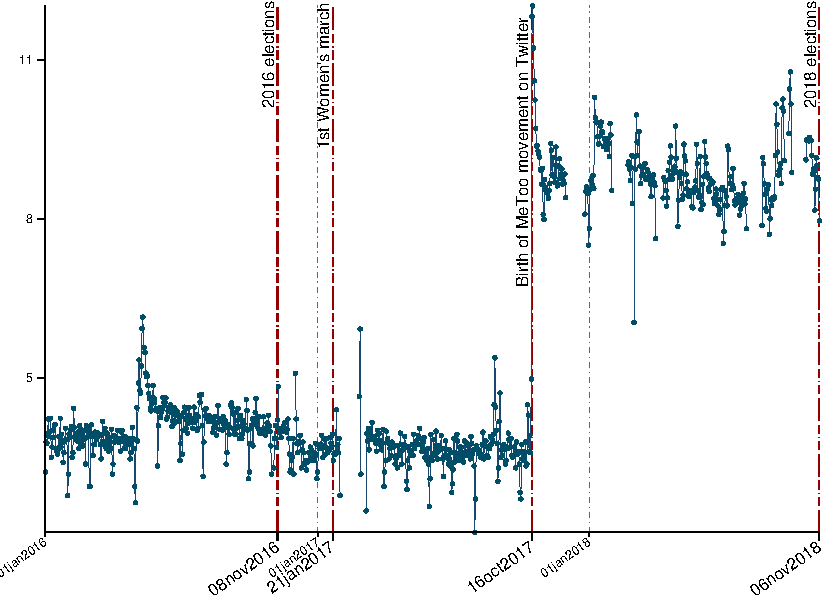
\includegraphics[width=0.9\textwidth]{figures/tweets-ts-2016to18.pdf}\vspace{-1em}
	\caption{
		Extended Timeline of MeToo Tweets.
		This figure shows the time series of the log tweet density, as in \cref{fig:tweets-ts}, but is extended back to 2016 to show the difference in the movement's strength.
	}
	\label{fig:tweets-ts-2016to18}
\end{figure}

First, \cref{tab:voteshare-2016} reports the result from estimating the same regression specification as in \cref{eq:voteshare}, aside from the temporal switch to 2016 in the dependent variable.
Overall, the 2016 estimates from are similar to those from 2018 \cref{tab:voteshare}. 
Areas where Democratic candidates in the 2018 House elections appear to benefit from the MeToo movement are also areas where Democratic candidates had an advantage in the 2016 House elections before the MeToo movement reached its peak (\cref{fig:tweets-ts-2016to18}).

Second, I examine women candidacy in 2016 (\cref{tab:candidacy-2016}) using the same regression specification as in \cref{eq:candidacy}.
The estimates (i) confirm the intra-party political norms discouraging women from challenging male incumbents from the same party in both 2016 and 2018, (ii) confirm that the weakening of these norms in districts with stronger MeToo activity is unique to 2018, as this interaction is absent in 2016 ($0.037$, $p > .1$), and (iii) reveal pre-existing geographic patterns where Republican women candidates in 2016 are more likely to challenge Democratic male incumbents but less likely to challenge Republican male incumbents in districts with high MeToo-related Twitter activity, consistent with the underlying demographic trends documented in the 2016 vote share analysis (\cref{tab:voteshare-2016}).

\begin{table}[ht]
\centering 
\footnotesize 
\setlength\tabcolsep{4 pt} \setlength{\defaultaddspace}{-1pt}
\def\sym#1{\ifmmode^{#1}\else\(^{#1}\)\fi}
\caption{The MeToo Movement and Candidate Vote Share, 2016 House Elections}
\label{tab:voteshare-2016}
\begin{adjustbox}{max width=1\textwidth}
	\begin{tabular}{@{\hspace{0\tabcolsep}}l*{4}{D{.}{.}{-1}}@{\hspace{0\tabcolsep}}}
		\toprule\toprule
		&&&\multicolumn{2}{c}{Heterogeneous effect, by pres.}\\
		&&&\multicolumn{2}{c}{\R{} vote share in 2016}\\
		\cmidrule(l){4-5}
		&\multicolumn{3}{c}{All-party share}&\multicolumn{1}{c}{Two-party share}\\
		\cmidrule(lr){2-4}\cmidrule(l){5-5}
		&\multicolumn{1}{c}{(1)}&\multicolumn{1}{c}{(2)}&\multicolumn{1}{c}{(3)}&\multicolumn{1}{c}{(4)}\\
		\midrule
		Log tweet density $ \times $ (Rep. woman)         &   -2.604\sym{**} &    0.073         &    0.912         &    1.239         \\
                                                  &  (1.018)         &  (0.709)         &  (1.187)         &  (1.151)         \\
Log tweet density $ \times $ (Dem. woman)         &    2.104\sym{***}&   -0.100         &   -0.885\sym{**} &   -1.021\sym{***}\\
                                                  &  (0.501)         &  (0.327)         &  (0.355)         &  (0.346)         \\
Log tweet density $ \times $ (Rep. man)           &   -2.081\sym{***}&    0.212         &    0.602\sym{**} &    0.163         \\
                                                  &  (0.646)         &  (0.153)         &  (0.251)         &  (0.280)         \\
Log tweet density $ \times $ (Dem. man)           &    1.874\sym{***}&   -0.116         &   -0.634\sym{*}  &   -0.693\sym{**} \\
                                                  &  (0.485)         &  (0.235)         &  (0.343)         &  (0.335)         \\
Log tweet density $ \times $ (Pres. 2016 Rep. vote share) $ \times $ (Rep. woman)&                  &                  &   -0.050         &   -0.062         \\
                                                  &                  &                  &  (0.049)         &  (0.048)         \\
Log tweet density $ \times $ (Pres. 2016 Rep. vote share) $ \times $ (Dem. woman)&                  &                  &    0.048\sym{***}&    0.049\sym{***}\\
                                                  &                  &                  &  (0.017)         &  (0.017)         \\
Log tweet density $ \times $ (Pres. 2016 Rep. vote share) $ \times $ (Rep. man)  &                  &                  &   -0.029\sym{***}&   -0.023\sym{*}  \\
                                                  &                  &                  &  (0.011)         &  (0.013)         \\
Log tweet density $ \times $ (Pres. 2016 Rep. vote share) $ \times $ (Dem. man)  &                  &                  &    0.037\sym{**} &    0.046\sym{***}\\
                                                  &                  &                  &  (0.016)         &  (0.016)         \\
\emph{Control variables}                          &                  &                  &                  &                  \\
\hspace{1em}Candidate fixed effects               &\multicolumn{1}{c}{$ X $}         &\multicolumn{1}{c}{$ X $}         &\multicolumn{1}{c}{$ X $}         &\multicolumn{1}{c}{$ X $}         \\
\hspace{1em}2008--12 Pres. election               &                  &\multicolumn{1}{c}{$ X $}         &\multicolumn{1}{c}{$ X $}         &\multicolumn{1}{c}{$ X $}         \\
\hspace{1em}County census demographics            &                  &\multicolumn{1}{c}{$ X $}         &\multicolumn{1}{c}{$ X $}         &\multicolumn{1}{c}{$ X $}         \\
\hspace{1em}Racial \& gender voting               &                  &\multicolumn{1}{c}{$ X $}         &\multicolumn{1}{c}{$ X $}         &\multicolumn{1}{c}{$ X $}         \\
Main-party candidates only                        &                  &                  &                  &\multicolumn{1}{c}{$ X $}         \\
$ N $                                             &\multicolumn{1}{c}{$ 5938 $}         &\multicolumn{1}{c}{$ 5936 $}         &\multicolumn{1}{c}{$ 5936 $}         &\multicolumn{1}{c}{$ 4508 $}         \\
		\bottomrule
	\end{tabular}
\end{adjustbox}
\caption*{
	\footnotesize
	\emph{Notes:}
	The dependent variable is the district-county-level 2016 house candidate vote share \citep{mitCountyHouse2016}, serving as a placebo outcome.
	Tweet density is the (natural) log of MeToo tweets in 2018 divided by county population.
	Past electoral results include the 2008 and 2012 presidential \R{} vote share, and the 2014 \R{} house vote share.
	All controls are otherwise the same as in Table \ref{tab:voteshare}.
	Candidates cluster robust standard errors in parentheses.
	Significance levels: $^*$ 0.1 $^{**}$ 0.05 $^{***}$ 0.01.
}
\end{table}
	
\begin{table}[ht]
	\centering
	\setlength\tabcolsep{8 pt} 
	\setlength{\defaultaddspace}{0pt}
	\def\sym#1{\ifmmode^{#1}\else\(^{#1}\)\fi}
	\caption{The MeToo Movement and Candidacy as Strategic Reaction (2016)}
	\label{tab:candidacy-2016}
	\begin{adjustbox}{max width=1\textwidth}
		\begin{tabular}{@{\hspace{0\tabcolsep}}l*{4}{D{.}{.}{-1}}@{\hspace{0\tabcolsep}}}
			\toprule\toprule
			&\multicolumn{4}{c}{Outcome is women challenger from the}\\
			\cmidrule{2-5}
			&\multicolumn{2}{c}{Republican party}&\multicolumn{2}{c}{Democratic party}\\
			\cmidrule(r){2-3} \cmidrule(l){4-5}
			&\multicolumn{1}{c}{(1)}&\multicolumn{1}{c}{(2)}&\multicolumn{1}{c}{(3)}&\multicolumn{1}{c}{(4)}\\
			\midrule
			Log tweet density   &   0.041\sym{**} &   0.006         &  -0.029         &  -0.012         \\
                    & (0.018)         & (0.015)         & (0.024)         & (0.037)         \\
Republican man incumbent&  -0.112\sym{***}&                 &   0.188\sym{***}&                 \\
                    & (0.027)         &                 & (0.051)         &                 \\
Democratic man incumbent&                 &   0.049         &                 &  -0.191\sym{***}\\
                    &                 & (0.038)         &                 & (0.047)         \\
Log tweet density $ \times $ (Republican man incumbent)&  -0.063\sym{***}&                 &   0.107\sym{***}&                 \\
                    & (0.023)         &                 & (0.036)         &                 \\
Log tweet density $ \times $ (Democratic man incumbent)&                 &   0.052\sym{**} &                 &   0.037         \\
                    &                 & (0.023)         &                 & (0.037)         \\
State fixed effects &\multicolumn{1}{c}{$ X $}         &\multicolumn{1}{c}{$ X $}         &\multicolumn{1}{c}{$ X $}         &\multicolumn{1}{c}{$ X $}         \\
Census Control      &\multicolumn{1}{c}{$ X $}         &\multicolumn{1}{c}{$ X $}         &\multicolumn{1}{c}{$ X $}         &\multicolumn{1}{c}{$ X $}         \\
F-test: Electoral controls = 0&\multicolumn{1}{c}{$ F = 1.69 $}         &\multicolumn{1}{c}{$ F = 1.74 $}         &\multicolumn{1}{c}{$ F = 2.84^{**} $}         &\multicolumn{1}{c}{$ F = 3.46^{**} $}         \\
F-test: County census = 0&\multicolumn{1}{c}{$ F = 4.35^{***} $}         &\multicolumn{1}{c}{$ F = 3.54^{***} $}         &\multicolumn{1}{c}{$ F = 2.69^{**} $}         &\multicolumn{1}{c}{$ F = 3.05^{**} $}         \\
$ R^2 $             &   0.266         &   0.247         &   0.209         &   0.195         \\
$ N $               &\multicolumn{1}{c}{$ 392 $}         &\multicolumn{1}{c}{$ 392 $}         &\multicolumn{1}{c}{$ 392 $}         &\multicolumn{1}{c}{$ 392 $}         \\
			\bottomrule
		\end{tabular}
	\end{adjustbox}
	\caption*{
		\footnotesize
		\emph{Notes:}
		The dependent variable is an indicator for the presence of a woman challenger from each party in the district for the 2016 House elections.
		Estimates are from linear probability models (\cref{eq:candidacy}).
		The log tweet density measure is mean-centered.
		Columns (1)--(2) examine Republican women challengers; columns (3)--(4) examine Democratic women challengers.
		Odd-numbered columns condition on Republican male incumbency; even-numbered columns condition on Democratic male incumbency.
		Robust standard errors clustered by state.
		Significance levels: $^*$ 0.1 $^{**}$ 0.05 $^{***}$ 0.01.
	}
\end{table}

\clearpage
\FloatBarrier
%-------------------------------------------------------------------------------
\section{Density vs. Intensity}
\label{sm:density-intensity}
%-------------------------------------------------------------------------------
This appendix compares estimates based on the tweet density measure (tweets per county population) with those based on the tweet intensity measure (without normalization).
The three tables present the three key results for candidate-level vote share (\cref{sec:voteshare-estimation}), district-level women candidacy (\cref{sec:candidacy-estimation}), and county-level voter turnout (\cref{sec:voteshare-estimation}).
Each table presents two columns for tweet density vs. tweet intensity, with both measures z-standardized (mean 0, SD 1) for comparison.
Specifications are otherwise identical (\crefrange{eq:repPres}{eq:turnout}).
The key observation across all tables (\crefrange{tab:voteshare-density-intensity}{tab:turnout-density-intensity}) is that, while the key estimates differ in magnitude, they are similar in direction and the level of statistical significance.

\begin{table}[ht] 
	\centering \scriptsize \setlength\tabcolsep{6 pt} \setlength{\defaultaddspace}{0pt}
	\def\sym#1{\ifmmode^{#1}\else\(^{#1}\)\fi}
	\caption{The MeToo Movement and Candidate Vote Share}
	\label{tab:voteshare-density-intensity}
	\begin{adjustbox}{max width=1\textwidth}
		\begin{tabular}{@{\hspace{0\tabcolsep}}l*{2}{D{.}{.}{-1}}@{\hspace{0\tabcolsep}}}
			\toprule\toprule
			&\multicolumn{1}{c}{Density}&\multicolumn{1}{c}{Intensity}\\
			&\multicolumn{1}{c}{(1)}&\multicolumn{1}{c}{(2)}\\
			\midrule
			MeToo tweets $ \times $ (Rep. woman)&   -0.078         &   -2.270         \\
          &  (1.491)         &  (2.112)         \\
MeToo tweets $ \times $ (Dem. woman)&   -1.202         &   -4.659\sym{***}\\
          &  (0.775)         &  (0.922)         \\
MeToo tweets $ \times $ (Rep. man)&    0.214         &   -1.923\sym{**} \\
          &  (0.573)         &  (0.769)         \\
MeToo tweets $ \times $ (Dem. man)&   -1.642\sym{**} &   -6.148\sym{***}\\
          &  (0.742)         &  (0.820)         \\
MeToo tweets $ \times $ (Pres. 2016 Rep. vote share) $ \times $ (Rep. woman)&   -0.064         &   -0.136\sym{**} \\
          &  (0.041)         &  (0.062)         \\
MeToo tweets $ \times $ (Pres. 2016 Rep. vote share) $ \times $ (Dem. woman)&    0.085\sym{**} &    0.224\sym{***}\\
          &  (0.034)         &  (0.038)         \\
MeToo tweets $ \times $ (Pres. 2016 Rep. vote share) $ \times $ (Rep. man)  &   -0.017         &   -0.054\sym{**} \\
          &  (0.019)         &  (0.024)         \\
MeToo tweets $ \times $ (Pres. 2016 Rep. vote share) $ \times $ (Dem. man)  &    0.058\sym{**} &    0.201\sym{***}\\
          &  (0.024)         &  (0.028)         \\
			\bottomrule
		\end{tabular}
	\end{adjustbox}
	\caption*{
		\footnotesize
		\emph{Notes:}
		This table replicates column (4) of \cref{tab:voteshare}, comparing density vs. intensity measures of the MeToo tweets.
		Column (1) uses log tweet density (tweets per capita). Column (2) uses log tweet intensity (raw tweet counts). Both tweet measures are standardized (mean 0, SD 1).
		Significance levels: $^*$ 0.1 $^{**}$ 0.05 $^{***}$ 0.01.
	}
\end{table}

\begin{table}[ht] 
	\centering \scriptsize \setlength\tabcolsep{6 pt} \setlength{\defaultaddspace}{0pt}
	\def\sym#1{\ifmmode^{#1}\else\(^{#1}\)\fi}
		\caption{The MeToo Movement and Candidacy as Strategic Reaction}
	\label{tab:candidacy-density-intensity}
	\begin{adjustbox}{max width=1\textwidth}
		\begin{tabular}{@{\hspace{0\tabcolsep}}l*{2}{D{.}{.}{-1}}@{\hspace{0\tabcolsep}}}
			\toprule\toprule
			&\multicolumn{1}{c}{Density}&\multicolumn{1}{c}{Intensity}\\
			&\multicolumn{1}{c}{(1)}&\multicolumn{1}{c}{(2)}\\
			\midrule
			MeToo tweets        &  -0.074         &  -0.105         \\
                    & (0.050)         & (0.074)         \\
Democratic man incumbent&  -0.417\sym{***}&  -0.440\sym{***}\\
                    & (0.055)         & (0.054)         \\
MeToo tweets $ \times $ (Democratic man incumbent)&   0.139\sym{***}&   0.175\sym{***}\\
                    & (0.042)         & (0.038)         \\
			\bottomrule
		\end{tabular}
	\end{adjustbox}
	\caption*{
		\footnotesize
		\emph{Notes:}
		This table replicates column (4) of \cref{tab:candidacy}, comparing density vs. intensity measures of the MeToo tweets.
		Column (1) uses log tweet density (tweets per capita). Column (2) uses log tweet intensity (raw tweet counts). Both tweet measures are standardized (mean 0, SD 1).
		Significance levels: $^*$ 0.1 $^{**}$ 0.05 $^{***}$ 0.01.
	}
\end{table}

\begin{table}[ht] 
	\centering \scriptsize \setlength\tabcolsep{6 pt} \setlength{\defaultaddspace}{0pt}
	\def\sym#1{\ifmmode^{#1}\else\(^{#1}\)\fi}
		\caption{The MeToo Movement and the Change in Voter Turnout}
	\label{tab:turnout-density-intensity}
	\begin{adjustbox}{max width=1\textwidth}
		\begin{tabular}{@{\hspace{0\tabcolsep}}l*{2}{D{.}{.}{-1}}@{\hspace{0\tabcolsep}}}
			\toprule\toprule
			&\multicolumn{1}{c}{Density}&\multicolumn{1}{c}{Intensity}\\
			&\multicolumn{1}{c}{(1)}&\multicolumn{1}{c}{(2)}\\
			\midrule
			MeToo tweets        &  0.0213         &  0.0355         \\
                    &(0.0211)         &(0.0381)         \\
Pres. 2016 Republican vote share& -0.0009         & -0.0005         \\
                    &(0.0044)         &(0.0045)         \\
MeToo tweets $ \times $ (Pres. 2016 Republican vote share)&  0.0000         &  0.0012\sym{*}  \\
                    &(0.0003)         &(0.0006)         \\
			\bottomrule
		\end{tabular}
	\end{adjustbox}
	\caption*{
		\footnotesize
		\emph{Notes:}
		This table replicates column (2) of \cref{tab:turnout}, comparing density vs. intensity measures of the MeToo tweets.
		Column (1) uses log tweet density (tweets per capita). Column (2) uses log tweet intensity (raw tweet counts). Both tweet measures are standardized (mean 0, SD 1).
		Significance levels: $^*$ 0.1 $^{**}$ 0.05 $^{***}$ 0.01.
	}
\end{table}

\FloatBarrier
\renewcommand{\refname}{Appendix References}
\putbib
\end{bibunit}
%TC:endignore
\end{document}
